%%%%%%%%%%%%%%%%%%%%%%%%%%%%%%%%%%%%%%%%%%%%%%%%%%%%%%%%%%%%%%%%%%%%%%%%%%%%%%%
%%%%%%%%%%%%%%%%%%%%%%%%%%%%%%%%%%%%%%%%%%%%%%%%%%%%%%%%%%%%%%%%%%%%%%%%%%%%%%%
%%%%  CHAPTER 1 
%%%%%%%%%%%%%%%%%%%%%%%%%%%%%%%%%%%%%%%%%%%%%%%%%%%%%%%%%%%%%%%%%%%%%%%%%%%%%%%
%%%%%%%%%%%%%%%%%%%%%%%%%%%%%%%%%%%%%%%%%%%%%%%%%%%%%%%%%%%%%%%%%%%%%%%%%%%%%%%

\chapter{Many body physics with ultracold atoms } 

\section{ Motivation:  Strongly correlated materials }

Most of our experiences in the physical world can, in principle, be explained
by considering the description of the collections of positively charged nuclei
and negatively charged electrons that make up ordinary matter.    From high to
low energy this includes: neutral plasmas,  free atoms, free  molecules, and
atoms and molecules that have condensed into liquid or glassy phases or
crystallized to form solids.   At lower energies more exotic phenomena take
place, starting with magnetism and going further to superfluidity,
superconductivity and the novel examples of modern condensed matter physics
such as the fractional quantum Hall effect, heavy electrons, high-temperature
superconductors and topological insulators.

In principle,  the correct description of all the above phenomena is contained
in the Schr\"{o}dinger equation for the interacting system of electrons and
nuclei,  where the interaction is given by the Coulomb potential. In practice,
we know that even though stating the equation is easy, there is not sufficient
computing power available in the world to solve it for systems of more than
just a few particles.  Xiao-Gang Wen, in the introduction to his textbook on
many-body physics~\cite{wen2004quantum}, points out that back in the 80's a
computer with 32 MB of RAM could solve a system of 11 interacting electrons.
In this century, while computing power has increased more than 100 times, this
allows for the addition of only two more electrons to the system.  

Despite the above,  the use of the Schr\"{o}dinger equation and perturbation
theory for the description of  systems of electrons and nuclei has been very
successful over the past century.  The most prominent example of this success
is our understanding of semiconductors, which are at the root of the electronic
devices that permeate all aspects of our lives.  The remarkable success of
condensed matter physics can be traced back to the principle of adiabatic
continuity~\cite{altland2010condensed}. This principle  states that  the
low-energy excitations of an interacting system  are  \textbf{non-interacting
quasiparticles} which can be closely related to the actual particles that form
the interacting system.   This last sentence may sound confusing, but think
about a hole in the valence band of a semiconductor.  The hole corresponds to a
collective arrangement of all the electrons in the system, but we typically do
not think about it that way.  The hole is a low energy excitation of the
collection of electrons, and thus we think about it as a
\textbf{quasiparticle}, with properties that are remarkably similar to those of
a free electron albeit with a positive rather than a negative charge.  The fact
that an electron and a hole behave so similarly is not at all intuitive,
especially if one stops to think about any effects due to the  Coulomb
interaction between electrons. However, adiabatic continuity guarantees that
for practical purposes we can think of the hole simply as a positively charged
electron.  

The practical consequence of adiabatic continuity is that interactions
seemingly do not play an important role in the low-energy description of the
system.  For this reason, the free electron model of Drude and
Sommerfeld~\cite{ashcroft1976solid} is relatively successful in explaining
electrical and thermal conductivity in metals,  and also in explaining the Hall
effect.   In 1957, Landau formulated the theory of the
Fermi-Liquid~\cite{landau1965collected} and gave a solid basis to the notion of
adiabatically connected quasiparticles.  To this day, the Fermi-Liquid theory
is the default starting point for the study of Fermi systems such as
conventional metals, helium-3, and ultracold atomic Fermi gases.   

But, just as Fermi-Liquid theory is celebrated for its success, it is also
known for the phenomena that it fails to explain.   Starting in the mid 70's
and going through the 80's, the discoveries of heavy electron
superconductivity~\cite{PhysRevLett.35.1779,PhysRevLett.43.1892},  the
fractional quantum Hall effect~\cite{PhysRevLett.48.1559,PhysRevLett.50.1395},
and high-temperature superconductors~\cite{Zeitschrift.64.189} sparked a
revolution in condensed matter physics~\cite{coleman2004revolution}.   These
materials, in which the electron behavior cannot be described effectively in
terms of non-interacting electron-like quasiparticles came to be known as
\textbf{strongly correlated materials}.   Strongly correlated materials, and
the concept of emergence, brought to the forefront by P.W.~Anderson in his
famous essay ``More is Different''~\cite{Anderson1972}, are at the center of
modern condensed matter physics. 

The behavior of strongly correlated materials is emergent because the
low-energy excitations of the system bear no resemblance to its constituent
particles.  This disconnect should not be so surprising, after all we are
familiar with this definition of emergence whenever a system undergoes a phase
transition.  For example, when a liquid cools down to form a crystalline solid,
continuous translational symmetry is broken.    By going across the
liquid-to-solid phase transition, adiabatic continuity is violated;
nevertheless, it is easy to mathematically identify the low energy excitations
of the new phase and ascribe them the character of quasiparticles.  In the case
of the crystalline solid this involves finding the normal modes of a set of
coupled oscillators; the normal modes are the quasiparticles known as phonons.
Phonons are emergent because they bear no direct resemblance to the constituent
ions that form the crystal lattice. 

Strongly correlated materials are examples of emergent phenomena in which the
origin and properties of the low-energy excitations are not as straightforward
as those of phonons in a crystalline solid.  The fractional quantum Hall state,
in which the quasiparticles carry a rational fraction of the electron charge
serves to illustrate this point.  The strong interactions between the electrons
in the quantum Hall system (electrons confined in a plane in the presence of a
very high magnetic field) make the problem intractable from the perturbative
point of view and thus \textbf{the connection between the microscopic degrees
of freedom and the collective low-energy excitations is very difficult to
establish}; certainly not as easy as the connection between small displacements
of ions about their equilibrium points in a crystal lattice and the collective
phonon modes. It was Laughlin's insight that led him to postulate the correct
wavefunction  for the quantum Hall state~\cite{PhysRevLett.50.1395}, but the
microscopic origin of the state is still under debate.   

The challenge posed by strongly correlated materials has led to great
discoveries in condensed matter physics, such as the concepts of topological
order~\cite{wen1990topological} and quantum
criticality~\cite{PhysRevB.14.1165,sachdev2011quantum}, but also many questions
remain unanswered.  Furthermore, the problem of strongly correlated materials
is only scratching the surface of what is possible and what remains to be
discovered.  New materials are being synthesized constantly.  Among the
myriad of possible materials and compounds yet to be explored by
materials scientists, one can only expect that there will be new states of
matter to be found; states with technological implications that will
revolutionize life on earth.  


\section{Quantum simulations with ultracold atoms}

We have seen that, even though the Schr\"{o}dinger equation in principle
contains a full description of a solid,  its solution is practically impossible
to compute using a classical computer due to the large amount of memory
required to represent a many-body quantum state.   
%Beyond this issue of scalability there is also the issue of interpretation of
%the results:  suppose that we were able to access the exact quantum state of
%the system and its time dependence,  what would we even do with such
%information?   It would be practically impossible to come up with experiments
%that could test the full validity of the state, thus making such knowledge
%superfluous since, after all, physics is an empirical endeavor.
The approach in condensed matter theory, rather than directly aim to solve the
complete Schr\"{o}dinger equation, is to introduce simplified effective models,
which should capture the essential features of the system under study.  Solving
the effective model leads to an understanding of the low-energy excitations of
the system and gives clues to their microscopic origin.   

The Hubbard model, formulated half a century ago~\cite{hubbard50} contains only
the essential ingredients necessary to describe the  behavior of strongly
interacting electrons moving in a periodic lattice. It describes electrons that
can hop between sites in a lattice (with probability amplitude $t$) , and which
acquire an interaction energy ($U$) when two electrons are on the same site,
see Figure~\ref{fig:chap01hubbard}.  
\begin{figure} \centering
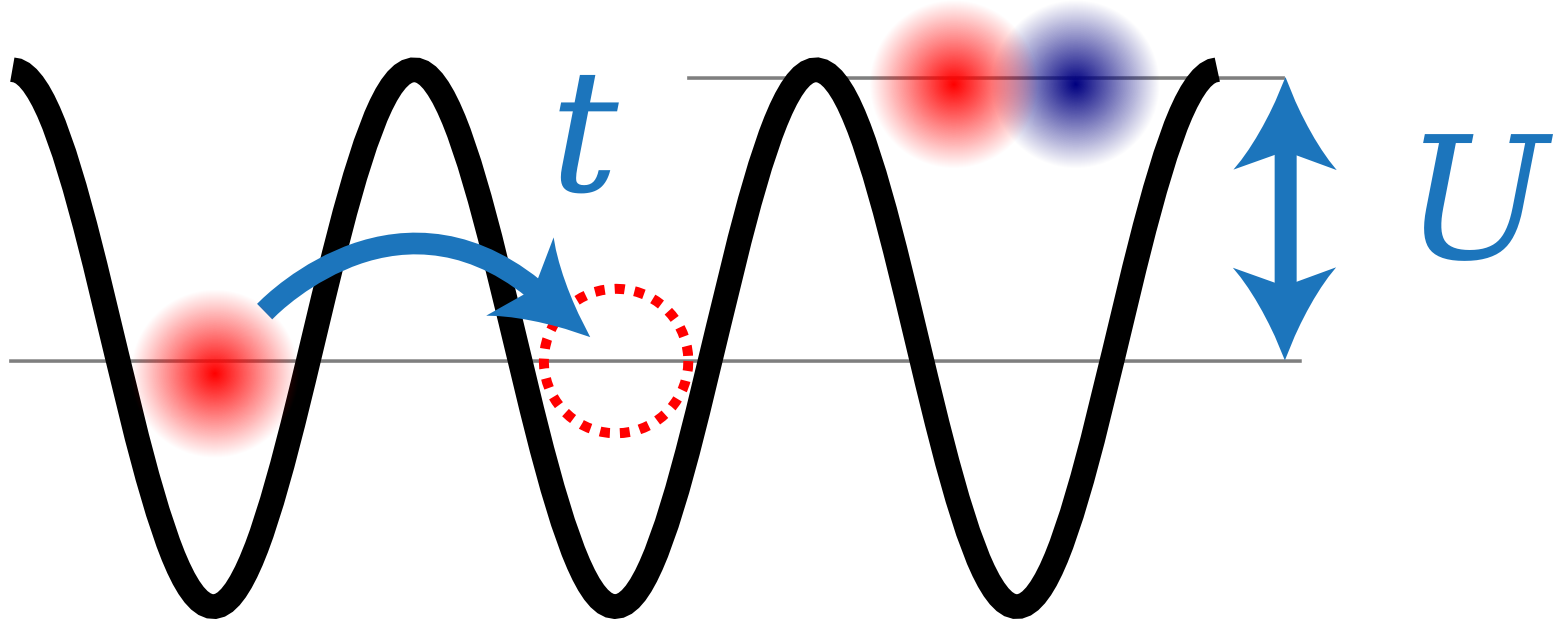
\includegraphics[width=0.4\textwidth]{../figures/hubbard/little-hubbard.png}
\caption[Hubbard model]{\small Illustration of the Hubbard model }
\label{fig:chap01hubbard}
\end{figure}
The Hubbard model is an extension of the tight-binding model, with the
interactions between electrons incorporated as the on-site energy $U$.
After its inception, it was shortly realized~\cite{Hubbard1964} that the model
could explain the Mott metal-insulator transition, which was observed in the
transition metal oxides even though conventional band theory predicted them to
be conductors.  Beyond its early success, the Hubbard model is now the
quintessential model for strongly correlated systems.  It is widely accepted as
the most viable candidate to explain high-$T_{c}$ superconductors from first
principles.   Despite this fact, its exact solution in more than one dimension
has evaded theorists for more than four decades~\cite{quintanilla2009strong}.

It is at this point that ultracold atoms enter the picture.   It turns out that
ultracold atoms in an optical lattice provide a faithful realization of the
Hubbard model~\cite{PhysRevLett.81.3108}, thus the properties exhibited by the
collection of atoms are in fact the solutions of the model.    In this way,
such systems can be used to map the phase diagram of the Hubbard model in what
is known as \textbf{quantum simulation}, an idea that was first proposed by
Richard Feynman in 1982~\cite{feynman1982simulating}. 

In a seminal paper~\cite{PhysRevLett.81.3108}, Jaksch and collaborators  showed
that Bose-Einstein condensates of atoms loaded into optical lattices could be
used as simulators of the Bose-Hubbard model.  A few years later, the
superfluid (SF) to Mott insulator (MI) phase transition, the hallmark of the
Bose-Hubbard model, was realized experimentally~\cite{Greiner2002}, and several
detailed studies of this system have followed since then~\cite{Gemelke2009,
Jimenez-Garcia2010, Trotzky2010, Mark2011, Zhang2012}.  For bosonic systems,
the properties of the ground state are well understood
theoretically~\cite{freericks1994bosehubbard, trivedi1991mott,
PhysRevB.40.546};  however, experiments on atoms in lattices are starting to
shed light into the dynamics of these systems~\cite{Fukuhara2013}, which are
more difficult to address for theorists.  

Despite the remarkable advances with bosonic systems, the ultimate goal of
quantum simulation with ultracold atoms is to find the ground states of
theoretically intractable fermionic models, to see if these models can
reproduce the measured properties of strongly correlated electron systems.  In
this prescription for quantum simulation, the subject of most interest is
whether or not the Hubbard model can exhibit a $d$-wave superfluid state which
would validate it as the prime model for high-$T_{c}$
superconductors~\cite{Scalapino1995329,PhysRevLett.89.220407}.  In pursuit of
this goal, experiments have realized the Hubbard model with spin mixtures of
fermionic atoms, where two hyperfine levels of the atomic ground state play the
role of spin-up and spin-down states of the spin-$\frac{1}{2}$ electrons in
real compounds.  Experiments with this kind of realization of the Hubbard model
are the subject of this thesis. 

A quantum degenerate spin-mixture of fermionic atoms is prepared in a harmonic
potential and then transferred adiabatically into an optical lattice potential.
The lattice depth and the contact interactions between the atoms, which
together set the values for the Hubbard parameters $t$ and $U$, can be
controlled almost at will by the experimenter.  The tunneling rate $t$ is
controlled  by adjusting the intensity of the lattice lasers.  The interaction
strength $U$ is controlled by setting the external magnetic field and making
use of a magnetically tunable Feshbach resonance, which offers the possibility
of realizing non-interacting samples, or samples with, arbitrarily, large
attractive or repulsive interactions\footnote{In practice it is observed that,
for some values of the interaction strength, significant three-body losses and
the associated heating rates prevent studying the equilibrium physics of the
quantum gas~\cite{PhysRevA.85.063615}.}.  The unprecedented control over the
system parameters has allowed the realization of band insulating
states~\cite{Kohl2005} and Mott insulating
states~\cite{Jordens2008,Schneider2008} with spin-mixtures of ultracold
fermionic atoms.  However, the possibility of exploring the strongly correlated
phases of the Hubbard model has not yet been realized because the required
temperatures are out of reach for current experiments.    


 
\section{Quantum magnetism with ultracold atoms }

Even though temperatures as low as $T\simeq 0.04\,T_{F}$ can be reached with
ultracold Fermi gases in a harmonic trap, these temperatures are not low enough
to allow exploration of the strongly correlated phases of the Hubbard model.
To get an idea of the temperature scales involved, we will examine a
qualitative temperature-doping 
%($T$-$x$) 
phase diagram, shown in Fig.~\ref{fig:cartoon-phasediag},  which is based on
experimental results obtained for the cuprate high-$T_{c}$
superconductors\footnote{See \cite{Damascelli2003} for a review of cuprate
superconductors, \cite{He2011} for a study of the onset of superconductivity at
optimal hole-doping, \cite{Jin2011} for the phase diagram of hole-doped cuprate
superconductors and \cite{Grant2011} for a more accessible report on the
subject.}, see Fig.~\ref{fig:cartoon-phasediag}.
\begin{figure} \centering
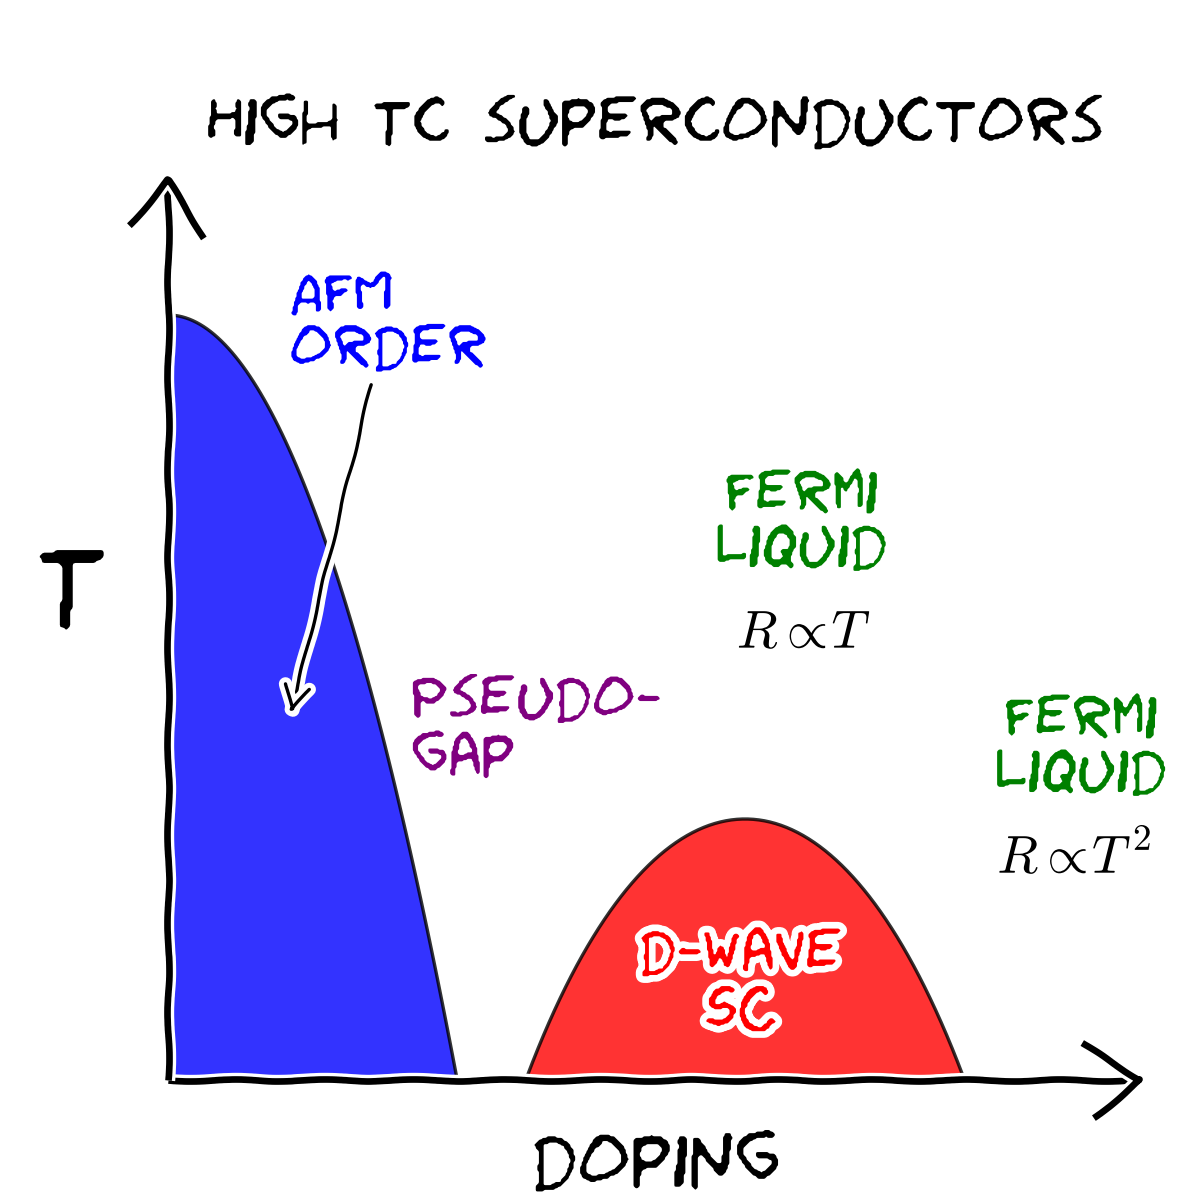
\includegraphics[width=0.4\textwidth]{../figures/hubbard/highTc.png}
\caption[Cartoon phase diagram for cuprate high-$T_{\text{C}}$
superconductors.]{\small Cartoon phase diagram for cuprate high-$T_{\text{C}}$
superconductors. The antiferromagnetic insulator (AFM) and the Fermi liquid
with quadratic resistivity are well understood by theory, however the strange
Fermi liquid with linear resistivity and the interplay between the pseudogap
regime and the superconducting dome are issues still under
debate~\cite{Grant2011}. }
\label{fig:cartoon-phasediag}
\end{figure}

The qualitative phase diagram shows that the cuprates exhibit various
interesting phases besides the superconducting (SC) dome at intermediate
doping.   Most importantly, the undoped parent compound is an antiferromagnetic
(AFM) Mott insulator with a N\'{e}el ordering temperature that is higher than
any value of the critical temperature $T_{\text{c}}$ along the SC dome.  

The onset of AFM ordering in the cuprate parent compounds is driven by the
magnetic exchange interaction~\cite{Koch2012}, where a spin can lower its
energy if it can tunnel virtually to a neighboring site.  For a single band
model, the Pauli exclusion principle dictates that this is only possible if
neighboring sites have opposing spins, as in the N\'{e}el AFM state.  The
N\'{e}el temperature $T_{N}$ is then of the order of the exchange energy
$4t^{2}/U$, which is the second-order correction (due to virtual tunneling)  to
the ground state energy of a two-site model in which the interaction $U$ is
treated as a perturbation.   The undoped parent compounds, at temperatures
several times larger than $T_{N}$, will be interaction driven Mott insulators
with exactly one electron per lattice site but without any spin ordering.  As
$T_{N}$ is approached, AFM correlations between the spins start to develop.  

To put some estimates on the values of $T_{N}$ and $T_{c}$, let's consider the
most common high-$T_{c}$ superconductor~\cite{Milton2010},
YBa$_{2}$Cu$_{3}$O$_{6+x}$, usually referred to as YBCO.  The critical
temperature for YBCO can be as large as $T_{c}\simeq 93$~K, obtained for
optimal hole-doping~\cite{Wu1987}. In the absence of doping, the YBCO parent
compound is antiferromagnetic with a N\'{e}el temperature $T_{N} \simeq 500
K$~\cite{Tranquada1988}.  The Fermi energy for YBCO is on the order of $\sim
1$~eV~\cite{liang2008ybco}, which corresponds to $\sim 10000$~K.  In units
of the Fermi temperature $T_{F}$, we have $T_{\text{C}}\simeq0.01\,T_{F}$,
and  $T_{\text{N}}\simeq0.05\,T_{F}$.

We immediately see that, in units of $T_{F}$,  the relevant temperature for
$d$-wave superconductivity is much lower than state-of-the-art temperatures for
ultracold fermionic atoms.  On the other hand $T_{N}$ may be just within reach.
The Mott insulator state (without spin ordering) was first realized with
fermionic atoms in a simple cubic lattice in
2008~\cite{Jordens2008,Schneider2008}.  Immediately after that, the race
started to see which group could be the first to observe the AFM state and take
the next step in the roadmap of quantum simulation.   

Recently in 2013, the Esslinger group, at ETH Z\"{u}rich, has demonstrated the
use of a dimerized optical lattice to measure the nearest-neighbor spin
correlations that start to develop, as a consequence of the exchange
interaction, at temperatures a few times larger than the N\'{e}el temperature
for AFM ordering~\cite{Greif2013}.  They observe significant spin-spin
correlations in arrays of one-dimensional chains, and they can detect the spin-spin
correlations that form on the approach to AFM order in a simple cubic lattice.
Prior to the work of the Esslinger group, the Bloch group used  a similar
optical super-lattice to study exchange interactions with bosons in isolated
double-wells~\cite{Trotzky2008} and isolated four-site
plaquettes~\cite{Nascimbene2012}. 

Other experiments have realized AFM states in engineered Ising Hamiltonians,
using trapped ions~\cite{Kim2010,Britton2012}, or by mapping motional degrees
of freedom to effective Ising models~\cite{Simon2011, Struck19082011}.  In
Ising type models, the magnetic coupling (anti or ferromagnetic) is put in by
hand in the Hamiltonian, and thus they realize what is referred to as
``classical'' magnetism.  In the Hubbard model, on the other hand,  magnetism
arises from the exchange interaction, as it does in condensed matter systems
such as the transition metal oxides or the cuprate parent compounds.
Realizations of classical magnetism are excellent systems to study magnetic
frustration, or the dynamics of quenching the system across a
phase-transition~\cite{PhysRevLett.111.053003}.   Systems of trapped ions can
help understand models with long range interactions~\cite{Richerme2014}, and
also emerge as good candidates to realize universal quantum
computers~\cite{Britton2012}.  Despite their advantages in other areas,
however, these systems do not directly address the long-standing open question
of superconductivity in the Hubbard model.


Approximately eight years ago, the Hulet lab started an experiment to study
strongly correlated matter using ultracold atoms in optical lattices; our main
goal being the achievement of temperatures below the N\'{e}el transition
temperature.  The N\'{e}el state in the Hubbard model,  besides being a
natural stepping stone in the quest to simulating strongly correlated systems,
offers the added benefit that it is well understood by theory~\cite{Paiva2011,
Fuchs2011}.   The ability to compare experimental results with theory offers a
test bed for quantum simulation and also a way to establish absolute
thermometry for ultracold atoms in optical lattices,  which is another major
challenge in this field~\cite{McKay2011}.  


%The absence of doping in the condensed matter system is
%equivalent to having a density of one atom per site in the ultracold atom
%system, also typically referred to as half-filling since the energy band has a
%total capacity of two atoms per site.  
%%The energy band has a total capacity of two atoms per site, so this $x=0$
%%point in the phase-diagram is also referred to as half-filling.   
%At half-filling, numerical approaches to the Hubbard model, such as
%determinantal quantum Monte Carlo (DQMC)~\cite{Paiva2011},  and dynamical mean
%field theory (DMFT)~\cite{Fuchs2011} do not suffer from the fermion sign
%problem~\cite{Jr1990}, and calculations can be performed down to temperatures
%below the N\'{e}el temperature for AFM ordering. 

\section{This thesis}

Over the course of this work we have used a compensated lattice potential,
which allows excellent control over the density distribution of the atoms in
the lattice.  The compensated lattice also helps mitigate heating of the atoms
as they are loaded into the lattice and has allowed us to reach temperatures as
low as 1.4~$T_{N}$, which is a factor of 2 colder than previous
experiments~\cite{Imriska2014}.  We measure the temperature of the atoms in the
lattice using Bragg scattering of light off of the magnetic sublattices that
start forming on the approach to the N\'{e}el transition.  This technique has
been discussed before~\cite{Ted2010}, but has not until now been implemented.
A very important aspect of our work is the comparison to \textit{ab initio}
numerical simulations of the Hubbard model.   We have used results from
determinantal quantum Monte Carlo (DQMC)~\cite{Paiva2011} and from numerical
linked-cluster expansion (NLCE)~\cite{Rigol2006} calculations,  along with the
local density approximation to establish the link between light scattering and
absolute thermometry of the sample. 

\subsection{Outline}

The approach taken in this thesis is to first provide a detailed description of
the condensed matter physics background which motivates our experiments, before
describing the experimental procedures and results.    

\begin{itemize}

\item Chapter~2 explains how ultracold atoms in an optical lattice can be an
almost ideal realization of the Hubbard model.   

\item Chapter~3 explores the
physics of the Hubbard model and gives the reader a flavor of the physics that
will be explored later on when discussing the results of our experiments. 

\item Chapter~4 introduces the experimental setup, to provide the context for the more detailed explanations that will follow.   

\item Chapter~5 discusses the optical lattice potential in which our
experiments are carried out.  We designed this potential with a few ideas in
mind regarding how it may help us reach lower temperatures with atoms in a
lattice.   Suggestions for future improvements of the setup will be given there.   

\item Chapters~6-9 describe the diagnostic tools that we have improved and
developed, over the course of this work, to access the physical observables in
our system.  

\item Chapter~10 gives details of a few crucial experimental steps required to
produce an ultracold gas of atoms in an optical lattice. 

\item Chapters 11 and
12 discuss the main results of this thesis:  the observation of an
incompressible Mott insulator of ultracold atoms in an optical lattice, and the
observation of antiferromagnetic correlations using Bragg scattering of light.

\item Chapter 13 concludes this thesis and discusses possible directions for
future experiments.  

\end{itemize}





%%%%%%%%%%%%%%%%%%%%%%%%%%%%%%%%%%%%%%%%%%%%%%%%%%%%%%%%%%%%%%%%%%%%%%%%%%%%%%%
%%%%%%%%%%%%%%%%%%%%%%%%%%%%%%%%%%%%%%%%%%%%%%%%%%%%%%%%%%%%%%%%%%%%%%%%%%%%%%%
%%%%  CHAPTER 2 
%%%%%%%%%%%%%%%%%%%%%%%%%%%%%%%%%%%%%%%%%%%%%%%%%%%%%%%%%%%%%%%%%%%%%%%%%%%%%%%
%%%%%%%%%%%%%%%%%%%%%%%%%%%%%%%%%%%%%%%%%%%%%%%%%%%%%%%%%%%%%%%%%%%%%%%%%%%%%%%

\chapter{Ultracold atoms in optical lattices}
\label{chap:atomsinlattices}

In this chapter we consider the description of cold atoms in an optical lattice
potential.    Second quantization is introduced, and the many-body Hubbard
Hamiltonian is derived, thus making the case for ultracold atoms as a nearly
ideal realization of the Hubbard model.  
% along the way we give a brief reminder of the treatment of interactions in
% cold atom gases.   
We discuss the requirements necessary for the ultracold atom system to be well
described by a single band Hubbard model. 

The computer code used to generate all of the plots in this chapter and to
calculate the Hubbard parameters $t$ and $U$ can be downloaded
from~\cite{PedroMDuarte:11612}. 


\section{One-dimensional optical lattice potential}

The contents of this section follow the derivation found in \S\,IV.A of the
review article by Morsch and Oberthaler.  \cite{RevModPhys.78.179}.  The
Hamiltonian for an atom moving in a one-dimensional (1D) sinusoidal potential,
such as that produced by an optical lattice, is 
\begin{equation}
  H_{\text{single,1D}} = 
  - \frac{\hbar^{2}}{2m} \frac{\partial^{2}}{\partial x^{2}} 
  + \vo\sin^{2}(kx) 
 \label{eq:Hsingle1D}
\end{equation}
where $k=2\pi/\lambda$, $\lambda$ is the wavelength of the lattice laser, and
$m$ is the mass of an atom.  The lattice depth \vo\ is naturally expressed in
units of the recoil energy: $\er=\frac{\hbar^{2}k^{2}}{2m}$.  Defining
$\vvo=\vo/\er$ the Hamiltonian reduces to  
\begin{equation}
\begin{split}
  H_{\text{single,1D}}= &
    -\frac{1}{k^{2}} \frac{\partial^{2}}{\partial x^{2}} 
    + \vvo\sin^{2}(kx) \\
           = &
    -\frac{1}{k^{2}} \frac{\partial^{2}}{\partial x^{2}} 
    + \frac{\vvo}{4}(2 - e^{2ikx} - e^{-2ikx} )  \\
\end{split}
\end{equation}
The solutions to the time independent Schr\"{o}dinger equation for this
Hamiltonian are Bloch states, which are labeled by their quasimomentum $q$ and
their band index $n$, and can be written in general form as 
\begin{equation}
  \psi_{q}^{n}(x) = e^{iqx} \sum_{l \in \mathbb{Z}} c_{ql}^{n} e^{ilGx}
  \label{eq:blochstate}
\end{equation}
The lattice translation invariant function that accompanies $e^{iqx}$ in a
Bloch state has been written here, with no loss of generality, as a sum of
plane waves with momenta $lG$,  where $l$ is an integer, $G=2k=2\pi/a$  is the
magnitude of the primitive vector of the reciprocal lattice,  and $a=\lambda/2$
is the lattice spacing. 

Acting with the Hamiltonian on the Bloch states and then rearranging some of
the terms in the infinite sum, we get \begin{equation}
\begin{split}
  H_{\text{single,1D}} \psi_{q}(x) = &  
      \sum_{l} \left[(q/k+2l)^{2} 
      + \frac{\vvo}{4}(2-e^{2ikx}-e^{-2ikx}) \right]
      c_{ql}^{n} e^{iqx+il2kx} \\ 
                                  = &  
      \sum_{l} \left[ \left(  (q/k+2l)^{2} 
      + \frac{\vvo}{2} \right) c_{ql}^{n} 
      - \frac{\vvo}{4}c_{q,l-1}^{n} - \frac{\vvo}{4}c_{q,l+1}^{n} \right] 
      e^{iqx+il2kx} 
\end{split}
\end{equation}
The quasimomentum is restricted to the first Brillouin zone, which can be taken
to be $[-\frac{\pi}{a}, \frac{\pi}{a})$.  The natural unit for the
quasimomentum is $2\pi/a$ ($=2k$).  Defining $q'=q/(2k)$,  we can then write
the time-independent Schr\"{o}dinger equation as 
\begin{equation}
  \left(  (2q'+2l)^{2} + \frac{\vo}{2} \right) c_{ql}^{n}
  - \frac{\vo}{4}c_{q,l-1}^{n} - \frac{\vo}{4}c_{q,l+1}^{n} = E_{q} c_{ql}^{n} 
\end{equation}
We then have an infinite linear system of equations which determines the
$c_{ql}^{n}$. For our practical purposes we truncate the set of equations such
that $|l|\leq\mathcal{N}$.  The resulting equations can be written in matrix form,
for example if we select $\mathcal{N}=2$ 
\begin{equation}
\left[\begin{smallmatrix}\frac{1}{2} V_{{0}} + 4 \left(q -2\right)^{2} & -
\frac{1}{4} V_{{0}} & 0 & 0 & 0\\- \frac{1}{4} V_{{0}} & \frac{1}{2} V_{{0}} +
4 \left(q -1\right)^{2} & - \frac{1}{4} V_{{0}} & 0 & 0\\0 & - \frac{1}{4}
V_{{0}} & \frac{1}{2} V_{{0}} + 4 q^{2} & - \frac{1}{4} V_{{0}} & 0\\0 & 0 & -
\frac{1}{4} V_{{0}} & \frac{1}{2} V_{{0}} + 4 \left(q + 1\right)^{2} & -
\frac{1}{4} V_{{0}}\\0 & 0 & 0 & - \frac{1}{4} V_{{0}} & \frac{1}{2} V_{{0}} +
4 \left(q + 2\right)^{2}\end{smallmatrix}\right] 
%
\cdot
\left[\begin{smallmatrix} 
  c_{q,-2}^{n} \\ 
  c_{q,-1}^{n} \\ 
  c_{q,0}^{n} \\ 
  c_{q,1}^{n} \\ 
  c_{q,2}^{n} \\ 
 \end{smallmatrix}\right]
 = E_{q}^{n} 
\left[\begin{smallmatrix} 
  c_{q,-2}^{n} \\ 
  c_{q,-1}^{n} \\ 
  c_{q,0}^{n} \\ 
  c_{q,1}^{n} \\ 
  c_{q,2}^{n} \\ 
 \end{smallmatrix}\right]
\label{eq:h1dmatrix} 
\end{equation}
These equations can be solved to obtain the eigenvectors $c_{ql}^{n}$ and the
eigenvalues $E_{q}^{n}$.  In the numerical solution that we implemented  we
truncated the infinite set at $\mathcal{N}=5$.  We find that, to accurately
obtain the dispersion relationship for the $n^{\text{th}}$ band, you need
$\mathcal{N}\geq n+1$.  

\subsection{Band structure}

The eigenvalues  obtained from the solutions to Eq.~\ref{eq:h1dmatrix}
correspond to the energies $E_{q}^{n}$ as a function of quasimomentum $q$ and
band index $n$ and are referred to as the band structure.  We show the band
structure for a 1D lattice as a function of $q$ in Fig.~\ref{fig:bands1d}, and
also as a function of lattice depth in Fig.~\ref{fig:bands1d_V0} 
\begin{figure}
\centering 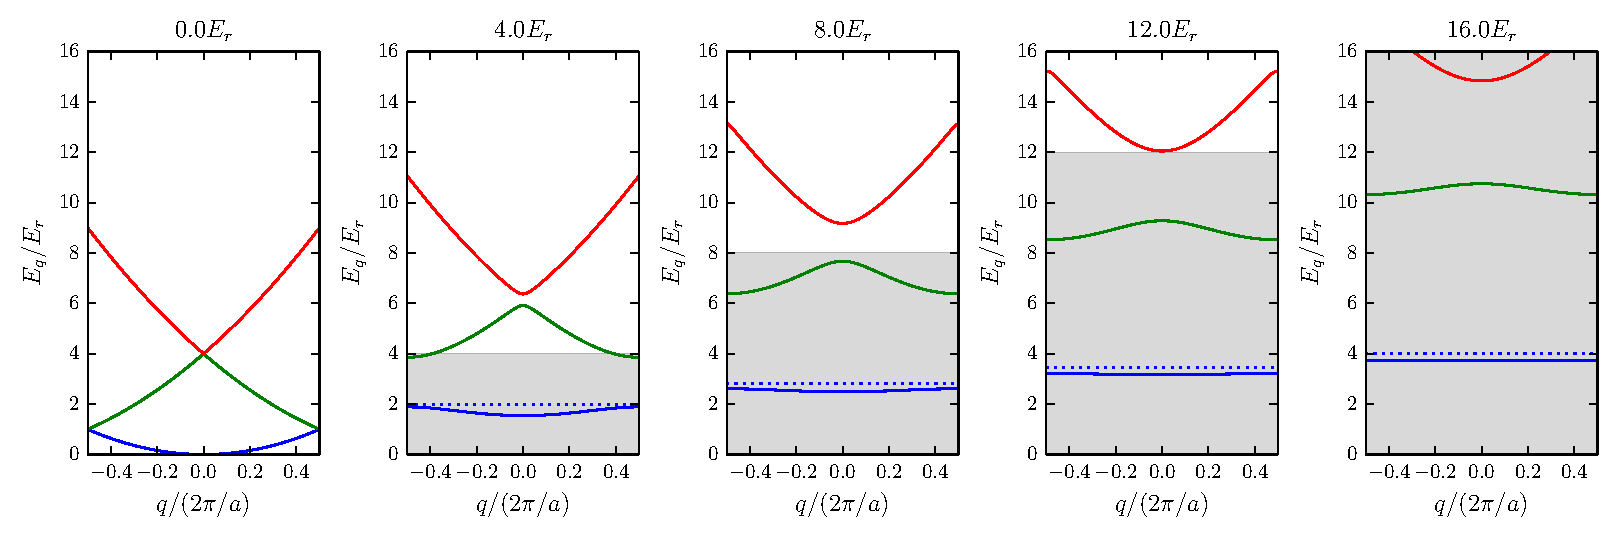
\includegraphics[width=\textwidth]{../figures/BandStructure_figures/bands1d.pdf}
\caption[Band structure in 1D lattice.]{\small Band structure in a 1D optical
lattice.  The depth of the lattice is indicated by the shaded area, and the
energy of the harmonic oscillator ground state in a single lattice site is shown
as a dotted line.  } \label{fig:bands1d}
\end{figure}
\begin{figure}
\centering 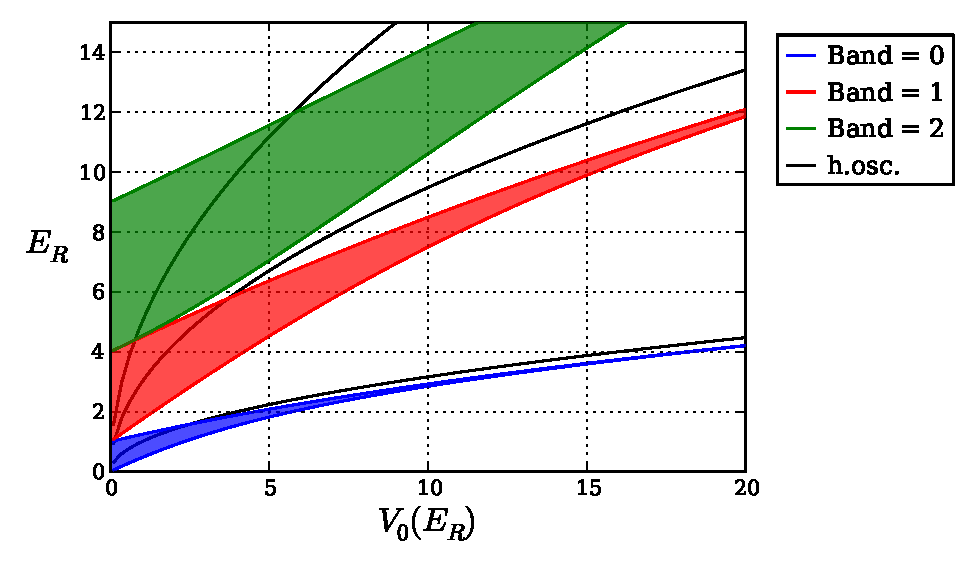
\includegraphics[width=0.6\textwidth]{../figures/BandStructure_figures/bands1d_V0.pdf}
\caption[Band structure in 1D lattice.]{\small Band structure in a 1D optical
lattice.  Each band is indicated by the colored area,  the harmonic oscillator
states in an isolated lattice site are shown as black lines. }
\label{fig:bands1d_V0}
\end{figure}

The time independent Schr\"{o}dinger equation for the Hamiltonian in
Eq.~\ref{eq:Hsingle1D}, can also be solved using Mathieu functions.  One can
then calculate the band structure by using the known properties of the Mathieu
functions, which are available on tables or as functions in some software
packages (e.g. Mathematica), see for instance the treatment
in~\cite{PhysRev.87.807}. 

\subsection{Eigenstates}
For each energy eigenvalue we have an associated eigenstate  which is defined
in terms of the $c_{ql}^{n}$ by Eq.~\ref{eq:blochstate}.   Typically, numerical
diagonalization routines return the normalized eigenvectors of the matrix in
question,  and for us this means that the coefficients $c_{ql}^{n}$ will
satisfy
\begin{equation}
   \sum_{l} | c_{ql}^{n} |^{2} = 1 
\end{equation} 
This has the implication that the states obtained from Eq.~\ref{eq:blochstate}
will be normalized over a lattice site.  In Fig.~\ref{fig:eigenfuns1d}. we show
the probability density for a lowest band eigenstate as a function of position
in the lattice for various lattice depths.  One can see how, as the lattice
gets deeper, the state becomes more localized around the center of each lattice
site. 
\begin{figure}
\centering 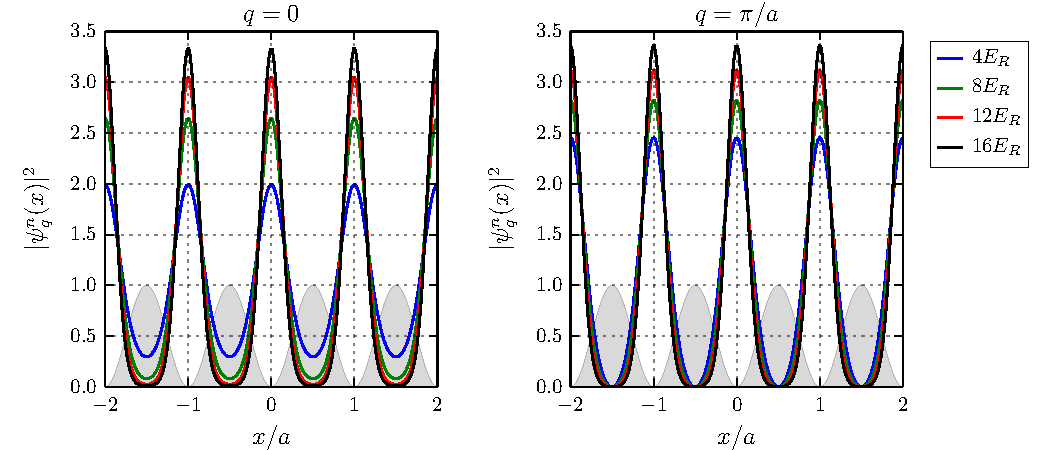
\includegraphics[width=\textwidth]{../figures/BandStructure_figures/eigenfuns1d.pdf}
\caption[Eigenstates in 1D lattice.]{\small Eigenstates of the Hamiltonian in a
1D optical lattice shown for $q=0$ (left) and $q=\pi/a$ (right) for various
lattice depths. The states are normalized so that the integral of the
probability density over one lattice site is equal to one.  The gray shaded
region is shown to indicate the variation of the lattice potential. }
\label{fig:eigenfuns1d}
\end{figure}

\subsection{Wannier states} 
\label{sec:1Dlattice}

It is useful to define a basis of states that are localized around a single
lattice site.  We will see later on that, when using such a basis, the
Hamiltonian for the Hubbard model takes its most familiar form.  In a finite
sized lattice with $L$ sites,  the localized state centered around the
$j^{\text{th}}$ site(at $x_{j}$) can be constructed as the following
superposition of eigenstates of the Hamiltonian\footnote{In some treatments
(for instance~\cite{salomon2013many}) the Wannier function is defined with a
normalization factor of $\sqrt{L}$  rather than $L$ as shown here.   Those
treatments consider eigenfunctions $\psi_{q}^{n}(x)$ which are normalized when
integrating over the full extent in the lattice.  We stick to the $L$
normalization factor, without the square root, since the eigenfunctions that
are obtained numerically come out normalized over a lattice site, as was
explained in the previous section.}: 
\begin{equation} w^{n}(x-x_{j}) =  \frac{1}{L} \sum_{q}  e^{-i q 2\pi x_{j} }
\psi_{q}^{n}(x) \label{eq:wannier} 
\end{equation} 
Here the sum runs over the
set of quasimomenta  $q \in \left\lbrace \frac{2\pi u}{a L} \ |\  u \in \lbrace
0,1,\ldots L-1 \rbrace \right\rbrace$.  Inserting the expansion of
$\psi_{q}^{n}(x)$ in plane waves into the definition of the Wannier state we
obtain 
\begin{equation}
 w^{n}(x-x_{j}) \equiv w_{j}^{n}(x)= 
    \frac{1}{L} \sum_{q}  
   \sum_{l \in \mathbb{Z}} 
   c_{ql}^{n} 
   e^{-i 2\pi q x_{j} }  
   e^{i 2\pi(q+l)x} 
\end{equation}
We will set $x_{j}=0$ for the calculation of the Wannier function,   Wannier
states centered at different lattice sites can be obtained by translation of
the $x_{j}=0$ solution. 
\begin{equation}
  w_{0}^{n}(x)= 
    \frac{1}{L} \sum_{q}  
   \sum_{l \in \mathbb{Z}} 
   c_{ql}^{n} 
   e^{i 2\pi(q+l)x} 
\end{equation}
Since the Hamiltonian commutes with the parity operator, it is required that
$\psi_{q}^{n}(-x) = \pm \psi_{q}^{n}(x)$, which implies that $c_{ql}^{n} = \pm
c_{pl'}^{n}$ if  $(q+l) = -(p+l')$.  Using this symmetry, the Wannier state
can be written as 
\begin{equation}
  w_{0}^{n}(x)= 
    \frac{1}{L} \left(
   c_{00}^{n} + 
    \sum_{q>0} 
   \sum_{l > 0 } 
   c_{ql}^{n} \left[ e^{i 2\pi(q+l)x} \pm e^{-i 2\pi(q+l)x } \right] \right)
\end{equation}
It is shown in~\cite{Kohn1959} that the maximally localized Wannier states are
obtained if the plus sign is chosen for even bands and the minus sign is chosen
for odd bands.  So, the $x_{j}=0$ Wannier state is symmetric for the even bands
and antisymmetric for the odd bands.  
\begin{equation}
  w_{0}^{n}(x)= 
    \frac{c_{00}^{n}}{L}
   + 
    \frac{2}{L}
    \sum_{q>0} 
   \sum_{l > 0 } 
   c_{ql}^{n} 
\begin{cases}
\cos[ 2\pi(q+l)x ] & \text{if $n$ even} \\
\sin[ 2\pi(q+l)x ] & \text{if $n$ odd }
\end{cases}
\end{equation}
%For $q,l>0$ all the coefficients $c_{ql}^{n}$ will have the same sign, so we
%select them to be positive.  

After defining the way to construct the Wannier states starting from the
$c_{ql}^{n}$, we can now proceed to add up the plane waves to  obtain the
states, as shown in Fig.~\ref{fig:wannier1d_V0} for various lattice depths.  As
the lattice depth is increased, the Wannier states become more localized, which
leads to less overlap between states in adjacent sites, and results in a
reduction of the probability amplitude for a particle to tunnel from one site
to the neighboring one.   More localized states also imply that the on-site
interaction will be larger, since, on average, two particles in the same site
will be closer to each other.  
\begin{figure}
\centering
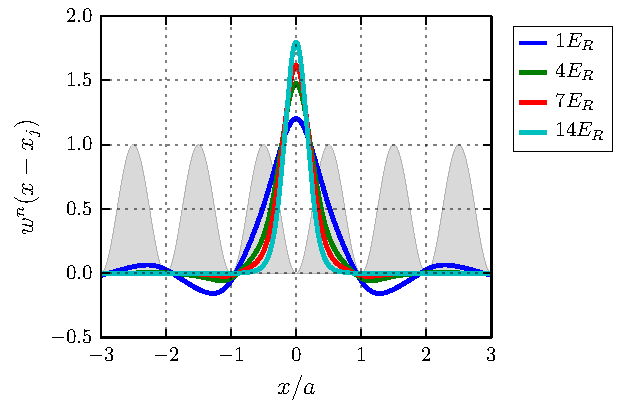
\includegraphics[width=0.6\textwidth]{../figures/BandStructure_figures/wannier1d_V0.pdf}
\caption[Wannier states in 1D lattice for various lattice depths.]{\small
Wannier states localized at $x_{j}=0$ in a 1D optical lattice for various
lattice depths.  The gray shaded region is shown to  indicate the spatial
variation of the lattice potential.  } \label{fig:wannier1d_V0}
\end{figure}

We also show, in Fig.~\ref{fig:wannier1d_bands}, the Wannier functions for the
first three bands in a 4$E_{R}$ lattice.  
\begin{figure}
\centering
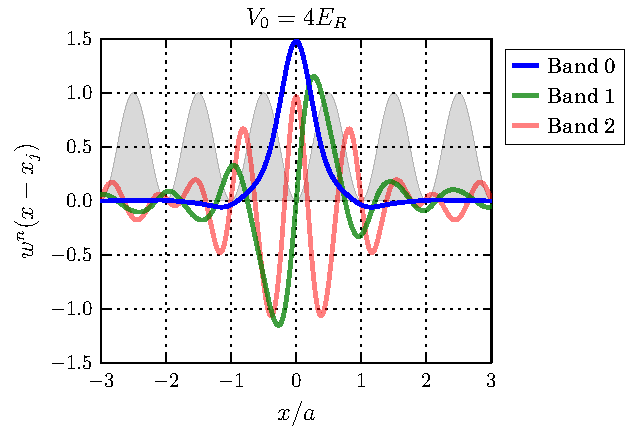
\includegraphics[width=0.6\textwidth]{../figures/BandStructure_figures/wannier1d_bands.pdf}
\caption[Wannier states in 1D lattice for the first three energy bands.]{\small
Wannier states localized at $x_{j}=0$  in a 4$E_{R}$ 1D optical lattice for the
first three energy bands.  The gray shaded region is shown to  indicate the
spatial variation of the lattice potential.  } \label{fig:wannier1d_bands}
\end{figure}

\section{Three-dimensional optical lattice potential}

The Hamiltonian for an atom moving in a  3D lattice can be separated in the
three spatial coordinates.  So we can use the solutions that were obtained in
the previous section for the 1D lattice and obtain the band structure and the
Wannier states for the 3D lattice.   The 3D band structure is shown in
Fig.~\ref{fig:bands3d_V0}. 
\begin{figure}
\centering 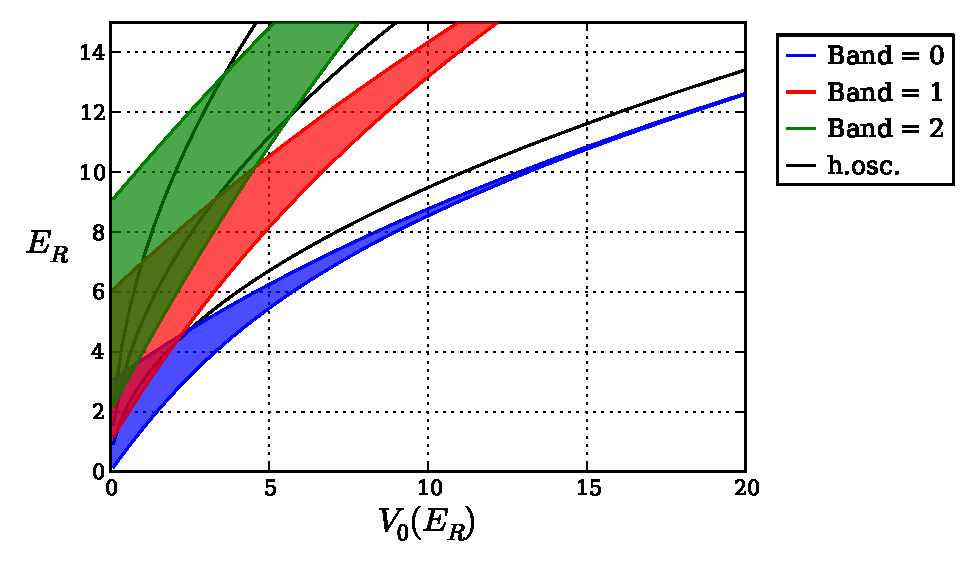
\includegraphics[width=0.6\textwidth]{../figures/BandStructure_figures/bands3d_V0.pdf}
\caption[Band structure in 3D lattice.]{\small Band structure in a 3D optical
lattice.  Each band is indicated by the colored area,  the harmonic oscillator
states in an isolated lattice site are shown as black lines. }
\label{fig:bands3d_V0}
\end{figure}

The Wannier states in a 3D lattice are simply products of the Wannier states in
each of the three spatial coordinates.  They are defined as 
\begin{equation}
 w^{n}(\bv{r}-\bv{r}_{j}) =  \frac{1}{L^{3}} \sum_{\bv{q}} e^{-i \bv{q}\cdot\bv{r}_{j} }
     \prod_{u=x,y,z}  \psi_{q_{u}}^{n_{u}}(u) 
 \label{eq:wannier3D}
\end{equation}
where $L^{3}$ is the total number of sites in the lattice. 

\section{Hubbard Hamiltonian}

The many-body Hubbard Hamiltonian is 
\begin{equation}
  H =  
-t \sum_{ \langle ij \rangle, \sigma   } 
          a_{i\sigma}^{\dagger}a_{j\sigma} \\
         + U\sum_{i} n_{i\spup} n_{i\spdn}  
\end{equation}
where $i,j$ are indices that run over lattice sites, $\langle ij \rangle$
denotes nearest-neighbors, and $\sigma$ denotes the spin state of the
particles.  The particle creation and annihilation operators,  $a_{j\sigma}$
and $a_{i\sigma}^{\dagger}$,  along with the number operator $n_{i\sigma}$
arise naturally in the second quantization formalism. In what follows, we will
see how to obtain this many-body form of the Hamiltonian, starting from the
first quantized version for a system of $N$ particles moving in a periodic
lattice. 


The Hamiltonian for a single atom in a 3D optical lattice is given by  
\begin{equation}
  H_{\text{single,3D}} = - \frac{\hbar^{2}}{2m} 
                 \left( \frac{\partial^{2}}{\partial x^{2}}
                            + \frac{\partial^{2}}{\partial y^{2}}
                            + \frac{\partial^{2}}{\partial z^{2}} \right)
 + \vo\left( \cos^{2}(kx)  + \cos^{2}(ky) + \cos^{2}(kz) \right)
\end{equation}
and when $N$ particles are considered, along with their interactions it takes a
more complicated form 
\begin{equation}
\begin{split}
  H = & \sum_{l}^{N}\left[ 
  -\frac{\hbar^{2}}{2m} \left( \frac{\partial^{2}}{\partial x_{l}^{2}}
                            + \frac{\partial^{2}}{\partial y_{l}^{2}}
                            + \frac{\partial^{2}}{\partial z_{l}^{2}} \right)
 + \vo\left( 
        \cos^{2}(kx_{l})  + \cos^{2}(ky_{l}) + \cos^{2}(kz_{l}) 
      \right) \right]\\
      &  + \frac{1}{2}\sum_{ l,n, l\neq n}^{N} 
              V_{\mathrm{int}}(\bv{r}_{l},\bv{r}_{n} )\\ 
    \equiv & ~ H_{0} + H_{\text{int}}
 \label{eq:hubbard1st}
\end{split} 
\end{equation} 
where the particles are labeled by indices $l$,$n$ and $V_{\mathrm{int}}$ is
the potential energy of interaction between two particles.  In the last line we
have defined a more concise notation that splits the Hamiltonian into the
non-interacting ($H_{0}$) and interacting ($H_{\text{int}}$) parts. Solving
this problem is a daunting task primarily for two reasons:
\begin{enumerate}
    \item The Bose or Fermi statistics of the identical particles under
consideration require the solutions to be fully symmetric or antisymmetric with
respect to particle exchange.
 
    \item The interactions between the particles prevent a straightforward
reformulation of the problem as a collection of easier-to-solve single particle
Hamiltonians.  
\end{enumerate}

The formalism of many-body theory encapsulates a series of methods to deal with
the two issues mentioned above.   First, the reformulation of the Schrodinger
equation in the language of second quantization provides the advantage that the
statistics are automatically taken into account by the notation, so one can
essentially forget about the the (anti)symmetrization of the many-particle wave
functions.  The small price to pay is that one needs to be very careful and
consistent about the order in which operators show up in the notation, since
the symmetry properties of the resulting states are contained in the
commutation relations defined between the operators.  Furthermore, second
quantization makes it easy to consider the extended Hilbert space where the
number of particles is not fixed, known as the Fock space. 

For weak interactions, many-body theory provides a solution to the problem in
terms of perturbation expansions for the physical quantities of interest.   The
theoretical formalism also reduces most of the important physical quantities in
terms of certain matrix elements (Green's functions). This allows the user to
concentrate on obtaining such matrix elements, which serve as a starting point
for the exploration of the properties of any system.   The complication arises
when the interactions are not weak, and the perturbative approach of the
many-body formalism breaks down.   


\subsection{Second quantization}

%The contents of this section comprise a short summary of the treatment in the
%books by Fetter and Walecka~\cite{fetter2003quantum} and
%Schwabl~\cite{schwabl2005advanced}.  

Let us start with a complete orthonormal set of single particle states $\lbrace
|i\rangle \rbrace \equiv \lbrace |1\rangle, |2\rangle, \ldots \rbrace$, using
these states we can write the basis states for the $N$-particle system as
\begin{equation}
   | i_{1}, \ldots i_{\alpha}, \ldots i_{N} \rangle \equiv 
   | i_{1}\rangle_{1} \ldots |i_{\alpha}\rangle_{\alpha} \ldots 
   | i_{N} \rangle_{N} ~,
\end{equation} 
which represents a state in which particle 1 is in state $i_{1} \in \lbrace
|i\rangle \rbrace$, particle $\alpha$ is in state $i_{\alpha}$ and so on.
These product states are not eigenstates of the permutation operator $P_{ij}$
which interchanges particles $i$ and $j$.  However, starting from the product
states we can obtain the completely (anti)symmetrized basis states for bosons
(fermions), which are eigenstates of any possible permutation of the
particle labels.  

For bosons, the normalized completely symmetric states are
\begin{equation} 
  | n_{1},  n_{2}, \ldots \rangle = 
  \frac{1}{\sqrt{N!n_{1}!n_{2}!\ldots}} \sum_{P}  
    P | i_{1},  i_{2}, \ldots i_{N} \rangle
\end{equation} 
where the $P$'s are elements of the permutation group\footnote{For $N$
particles there are $N!$ possible permutations and thus $N!$ elements in the
permutation group.}  In this expression, $n_{i}$ is the number of times that
the state $|i\rangle$ occurs among the $N$ particles, also called the
occupation number of state $|i\rangle$.  The sum of all occupation numbers
$n_{i}$ must equal the total number of particles, but otherwise there is no
restriction in the occupation number for bosons.

For fermions the normalized completely antisymmetric states have an extra
factor $(-1)^{P}$, which denotes the parity of the permutation $P$.  They can
be written in the form of Slater determinants: \begin{equation}
\begin{split}
  | n_{1},  n_{2}, \ldots \rangle = &
  \frac{1}{\sqrt{N!}} \sum_{P} (- 1)^{P} P |
                                 i_{1},  i_{2}, \ldots i_{N} \rangle \\
  = &
  \frac{1}{\sqrt{N!}}
  \begin{vmatrix}
  |i_{1}\rangle_{1} & |i_{1}\rangle_{2} & \dotsm & |i_{1}\rangle_{N} \\
  \vdots &  \vdots &  \ddots   & \vdots \\
  |i_{N}\rangle_{1} & |i_{N}\rangle_{2} & \dotsm & |i_{N}\rangle_{N} \\
\end{vmatrix}
\end{split} 
  \label{eq:antisymmetrize} 
\end{equation}  
If a single particle state appears more than once in the product state, the
resulting totally antisymmetric state is zero,  i.e. the occupation numbers
$n_{i}$ can only take the values 0 or 1, a consequence of the Pauli exclusion
principle. 

For bosons (fermions), we can combine the (anti)symmetric states for
$N=0,1,2,\ldots$ particles to obtain a complete orthonormal set of states for
arbitrary particle number.  This ``number states'' are the basis of the Fock
space. 


%We now define the creation  operators for bosons, which allow us to take a
%state from the subspace of $N$ particles, to the subspace of $N+1$  particles.
%\begin{equation}
% a_{i}^{\dagger} | \ldots, n_{i}, \ldots \rangle  = 
% \sqrt{n_{i}+1}|\ldots, n_{i}+1, \dots\rangle
%\end{equation}
%It follows that the adjoint of the creation operator is the annihilation
%operator and satisfies 
%\begin{equation}
%a_{i} | \ldots, n_{i}, \ldots \rangle  
%=\begin{cases}
%\sqrt{n_{i}}|\ldots, n_{i}-1, \dots\rangle
%& \text{if $n_{i}\geq 0$},\\
%0 & \text{if $n_{i}=0$}
%\end{cases}
%\end{equation}
%The creation and annihilation operators are defined such that one can create
%any state starting from the vacuum state $|0\rangle \equiv |0,0,\ldots\rangle$
%in which there are no particles at all.  In more formal terms 
%\begin{equation}
%  | n_{1}, n_{2}, \dots \rangle = \frac{1}{\sqrt{n_{1}!n_{2}!\ldots}} 
%   ( a_{1}^{\dagger} ) ^{n_{1}}  
%   ( a_{2}^{\dagger} ) ^{n_{2}}  \ldots | 0 \rangle
%  \label{eq:numberstate}
%\end{equation}
%The boson creation and annihilation operators satisfty the Bose communtation
%relations 
%\begin{equation}
%  [a_{i}, a_{j}] = 0 \ \ \ \ \  
%  [a_{i}^{\dagger}, a_{j}^{\dagger}] = 0 \ \ \ \ \   
%  [a_{i},a_{j}^{\dagger}]=\delta_{ij}
%\end{equation}

We will concentrate in the case of fermions, and define the creation operators
such that the number state can be written as 
\begin{equation}
 | n_{1}, n_{2}, \ldots \rangle = 
    \left( a_{1}^{\dagger}\right)^{n_{1}} 
    \left( a_{2}^{\dagger}\right)^{n_{2}} \ldots |0\rangle 
%    ~~~~~~ n_{i} = 0\ \text{or}\ 1  
\label{eq:defnumberstate0}
\end{equation}
where $|0\rangle$ is the vacuum state, in which there are no particles.  By
definition, the number state is completely antisymmetric, but what does this
imply for the creation operators?  Going back to Eq.~\ref{eq:antisymmetrize},
which defines the number states,  we see that the sign of the number state
depends on the particular ordering of the single particle states in the Slater
determinant.   Suppose $n_{1}=n_{2}=1$, changing the labels on states 1 and 2
corresponds to exchanging two rows in the Slater determinant and thus a minus
sign comes out: 
\begin{equation} 
    \left( a_{2}^{\dagger}\right)^{n_{2}} 
    \left( a_{1}^{\dagger}\right)^{n_{1}} \ldots |0\rangle  = 
  - | n_{1}, n_{2}, \ldots \rangle 
%    ~~~~~~ n_{i} = 0\ \text{or}\ 1  
\end{equation}
Comparing with Eq.~\ref{eq:defnumberstate0} we notice that the creation
operators must then satisfy the following anticommutation relation
\begin{equation} 
    a_{1}^{\dagger} a_{2}^{\dagger} + a_{2}^{\dagger} a_{1}^{\dagger} 
   \equiv  \left\lbrace  a_{1}^{\dagger} , a_{2}^{\dagger} \right\rbrace 
   = 0 
\end{equation}
Notice that this anticommutation relation implies $\left( a_{i}^{\dagger}
\right)^{2} = 0$, which is yet another manifestation of the Pauli exclusion
principle.
   
When dealing with fermions, one must decide first on a particular ordering of
the single particle states and then stick to it, noticing that to produce the
number states (without a minus sign) all the creation operators must be applied
to the vacuum state in the chosen order.   The action of a creation operator on
a number state is
\begin{equation}  
  a_{i}^{\dagger}| \ldots, n_{i}, \ldots \rangle 
  =    (-1)^{\sum_{k<i} n_{k}} | \ldots, n_{i}+1, \ldots \rangle 
 \label{eq:defcreation}
\end{equation} 
where the factor $(-1)^{\sum_{k<i} n_{k}}$ takes care of the number of
anticommutations needed to place the $a_{i}^{\dagger}$ operator in the correct
position.  The action of the fermion annihilation operators can be inferred by
taking the adjoint of Eq.~ \ref{eq:defcreation}.  One can then obtain all of
the anticommutation rules for fermions: 
\begin{equation}
  \left\lbrace a_{i}, a_{j} \right\rbrace = 0 \ \ \ \ \  
  \left\lbrace a_{i}^{\dagger}, a_{j}^{\dagger} \right\rbrace = 0 \ \ \ \ \   
  \left\lbrace a_{i},a_{j}^{\dagger} \right\rbrace=\delta_{ij}
\end{equation}


\subsection{Operators in second quantization}

So far two great leaps have been taken: 
\begin{enumerate}
 \item We have swept antisymmetrization under the rug by introducing the number
states, defined from the vacuum in terms of creation operators which satisfy
the Fermi anticommutation rules. 
 
 \item We started from an $N$ particle Hamiltonian, but we have now defined
number states that can handle the description of systems with an arbitrary
number of particles 
\end{enumerate}
The two ideas mentioned are related to the states used to describe the system,
now we will turn to the problem of the observables and see how they are handled
in the second quantization.  


Let us consider the sum $\sum_{\alpha} |i\rangle_{\alpha} \langle j | _{\alpha}
$ where $|i\rangle$ and $|j\rangle$ are single particle states, and $\alpha$
runs over all particles in the system.  We apply the sum to the number states
using the definition in Eq.~\ref{eq:antisymmetrize}: 
\begin{equation}
  \left(
   \sum_{\alpha} |i\rangle_{\alpha} \langle j | _{\alpha}  \right)
  | n_{1},  n_{2}, \ldots \rangle = 
  \frac{1}{\sqrt{N!}} \sum_{P} (- 1)^{P} P 
  \left( \sum_{\alpha} |i\rangle_{\alpha} \langle j | _{\alpha} 
   | i_{1},  i_{2}, \ldots i_{N} \rangle \right)
\end{equation}
For the term in the right not to vanish, the initial number state  must have a
particle in state $|j\rangle$, i.e. it must have $n_{j}=1$. Also, $n_{i}$ must
be $n_{i}=0$,  or else the completely antisymmetric state will vanish.  If the
particle initially in state $|j\rangle$ is labeled as  $J$  we can write
\begin{equation}
\begin{split}
  \left(
   \sum_{\alpha} |i\rangle_{\alpha} \langle j | _{\alpha}  \right)
  | n_{1},  n_{2}, \ldots \rangle = &
  \frac{1}{\sqrt{N!}} \sum_{P} (- 1)^{P} P \left( 
    |i_{1}\rangle_{1}
    |i_{2}\rangle_{2}
    \ldots 
     \!\!\!\!\!\!
    \underbrace{ 
    |i\rangle_{J} }_{\text{instead of } |j\rangle_{J}} 
     \!\!\!\!\!\!
    \ldots 
    |i_{N}\rangle_{N}
  \right) \\
   =&  
  \frac{1}{\sqrt{N!}}
  \begin{vmatrix}
  |i_{1}\rangle_{1} & |i_{1}\rangle_{2} & \dotsm & |i_{1}\rangle_{N} \\
  \vdots &  \vdots &     & \vdots \\
  |i\rangle_{1} & |i\rangle_{2} & \dotsm & |i\rangle_{N} \\
  \vdots &  \vdots &     & \vdots \\
  |i_{N}\rangle_{1} & |i_{N}\rangle_{2} & \dotsm & |i_{N}\rangle_{N} \\
\end{vmatrix} \\
\end{split} 
\end{equation}
In the determinant of the left, the state $|i\rangle$ appears in the
$j^{\text{th}}$ row, so a few rows need to be exchanged to put it in the
correct place, in accordance with our sign convention for the number states:
\begin{multline}
  \left(
   \sum_{\alpha} |i\rangle_{\alpha} \langle j | _{\alpha}  \right)
  | n_{1},  n_{2}, \ldots \rangle = \\  
 \begin{cases}
(-1)^{\sum_{k<j} n_{k} + \sum_{k<i}n_{k}~~~}
   \,| n_{1}, n_{2},  \ldots, n_{i}+1, \ldots,  n_{j}-1, \ldots  \rangle   
& \text{if $i\leq j$},\\
(-1)^{\sum_{k<j} n_{k} + \sum_{k<i}n_{k} -1 } 
   \,| n_{1}, n_{2},  \ldots, n_{j}-1, \ldots,  n_{i}+1, \ldots  \rangle
& \text{if $i>j$}
\end{cases}  
\end{multline}
Checking the definition of the creation and annihilation operators we obtain
the important result 
\begin{equation}
  \left(
   \sum_{\alpha} |i\rangle_{\alpha} \langle j | _{\alpha}  \right)
  | n_{1},  n_{2}, \ldots \rangle 
   =   a_{i}^{\dagger} a_{j} 
  | n_{1},  n_{2}, \ldots \rangle 
  ~~~~~ \Rightarrow ~~~~~ 
   \sum_{\alpha} |i\rangle_{\alpha} \langle j | _{\alpha} = 
     a_{i}^{\dagger} a_{j} 
\end{equation}

Now, consider an operator $T$ that is a sum over single particle operators
\begin{equation}
  T = \sum_{\alpha} t_{\alpha}
 \label{eq:defsingleparticleop}
\end{equation}  
If we insert the completeness relation for the single particle states twice in
this sum, we have \begin{equation}
\begin{split}
  T = & \sum_{\alpha} 
        \left( \sum_{i} |i\rangle_{\alpha}\langle i |_{\alpha} \right)
        t_{\alpha} 
        \left( \sum_{j} |j\rangle_{\alpha}\langle j |_{\alpha} \right) \\
    = & \sum_{ij}   \langle i | t | j \rangle  
          \sum_{\alpha} |i\rangle_{\alpha} \langle j |_{\alpha} \\ 
    = & \sum_{ij}   \langle i | t | j \rangle a_{i}^{\dagger} a_{j} 
          \equiv \sum_{ij} t_{ij}   a_{i}^{\dagger} a_{j} 
\end{split}  
\end{equation}
\textbf{This is the other big leap provided by the second quantization}:  an
operator that was written as a sum over particles becomes a sum of creation and
annihilation operators.   We will apply this prescription to the
non-interacting part of the Hamiltonian for $N$ particles moving in a lattice.  

Operators like the potential energy, $ \frac{1}{2}\sum_{l,n,l\neq n}^{N}
V_{\mathrm{int}}(\bv{r}_{l}, \bv{r}_{n} )$ , which are a sum over two-particle
(or many-particle) operators,  can be similarly expressed as sums of creation
and annihilation operators~\cite{schwabl2005advanced}.  For a two-body operator
we have the expression
\begin{equation}
\begin{split}
F = & \frac{1}{2} \sum_{\alpha\neq\beta} f(\bv{r}_{\alpha}, \bv{r}_{\beta} )  \\
  = & \frac{1}{2} \sum_{ijkm} \langle ij | f | km \rangle 
        a_{i}^{\dagger} a_{j}^{\dagger} a_{m} a_{k} 
\end{split}
\end{equation}

\subsection{Second quantized Hubbard Hamiltonian}

The Hubbard Hamiltonian in Eq.~\ref{eq:hubbard1st} is a sum of two
single-particle operators and one two-particle operator.  These are,
respectively: the kinetic energy, the energy of the atoms in the lattice
potential, and the interactions between the atoms.  In this section we will
express the Hubbard Hamiltonian in second quantized form.  As a single-particle
basis we will use the Wannier states that were derived in
Section.~\ref{sec:1Dlattice}

%In the Hubbard Hamiltonian the two single-particle operators are grouped
%together to define the non-interacting part of the Hamiltonian 
%\begin{equation}
%\begin{split}
%  H_{0} = & \sum_{l}^{N} -\frac{\hbar^{2}}{2m} 
%            \left( \frac{\partial^{2}}{\partial x_{l}^{2}}
%                            + \frac{\partial^{2}}{\partial y_{l}^{2}}
%                            + \frac{\partial^{2}}{\partial z_{l}^{2}} \right)
% + \vo\left( \cos^{2}(kx_{l})  + \cos^{2}(ky_{l}) + \cos^{2}(kz_{l}) \right) \\
%       = & \sum_{l}^{N} H_{\text{single,3D}}^{l}
%\end{split}
%\end{equation}

\paragraph{Tunneling matrix element, $\bm{t}$.} $H_{0}$ is a single particle
operator of the kind defined in Eq.~\ref{eq:defsingleparticleop}:
\begin{equation}
  H_{0} = 
     \sum_{l=1}^{N} H_{\text{single,3D}}^{l}
\end{equation}
where 
\begin{equation}
H_{\text{single,3D}}^{l} = 
  -\frac{\hbar^{2}}{2m} \left( \frac{\partial^{2}}{\partial x_{l}^{2}}
                            + \frac{\partial^{2}}{\partial y_{l}^{2}}
                            + \frac{\partial^{2}}{\partial z_{l}^{2}} \right)
 + \vo\left( \cos^{2}(kx_{l})  + \cos^{2}(ky_{l}) + \cos^{2}(kz_{l}) \right) 
\end{equation}
Its second quantized form can be written as 
\begin{equation}
\begin{split}
  H_{0} = & \sum_{ij} 
       \langle i| H_{\text{single,3D}} |j \rangle a_{i}^{\dagger} a_{j} \\
        \equiv & ~ -\sum_{ij} t_{ij}  a_{i}^{\dagger} a_{j} \\
\end{split}
\end{equation}  
Note that the sign of $t_{ij}$ was picked rather arbitrarily to follow the
usual conventions.  We now proceed to find the value of the matrix element
$t_{ij}$.  We use the definition of the Wannier states given in
Eq.~\ref{eq:wannier3D} to find 
\begin{equation}
\begin{split}
-t_{ij}  
= & 
  \frac{1}{L^{6}}\int \mathrm{d}\bv{r}\ 
     \sum_{\bv{q}'} e^{i \bv{q'}\cdot\bv{r}_{i} }
     \prod_{u'=x,y,z}  \psi_{q'_{u'}}^{n'_{u'}*}(u') 
  \Big( H_{\text{single,3D}}  \Big)
     \sum_{\bv{q}} e^{-i \bv{q}\cdot\bv{r}_{j} }
     \prod_{u=x,y,z}  \psi_{q_{u}}^{n_{u}}(u)\\ 
= &
  \sum_{\bv{q}\bv{q}'}   
  \frac{E_{\bv{q}}^{n}}{L^{6}}
   e^{ i \bv{q}'\cdot\bv{r}_{i} }  e^{ -i \bv{q}\cdot\bv{r}_{j} }
   \int\mathrm{d}\bv{r}\ 
     \prod_{u'=x,y,z}  \psi_{q'_{u'}}^{n'_{u'}*}(u') 
     \prod_{u=x,y,z}  \psi_{q_{u}}^{n_{u}}(u) \\ 
= &
  \sum_{\bv{q}\bv{q}'}   
  \frac{E_{\bv{q}}^{n}}{L^{6}}
   e^{ i \bv{q}'\cdot\bv{r}_{i} }  e^{ -i \bv{q}\cdot\bv{r}_{j} }
   \delta_{\bv{q}\bv{q}'} \delta_{nn'} L^{3} \\
= &
  \frac{1}{L^{3}}
  \sum_{\bv{q}}   E_{\bv{q}}^{n}
   e^{ i \bv{q}\cdot(\bv{r}_{i} - \bv{r}_{j}) } \delta_{nn'}\\
\end{split} 
\end{equation}
We observe that there is no amplitude to go between states that are in two
different bands, as is indicated by the appearance of $\delta_{nn'}$.   In what
follows, we will consider only the lowest band, $n=0$,  so we will drop the
band index, $n$, altogether.  For this simplification to be valid, the
following two requirements must be satisfied by the system:
 
\begin{enumerate}
\item \textbf{The temperature and the Fermi energy need to be small compared to
the energy gap between the lowest and first excited band.}

\item \textbf{The interaction energy scale must also be small compared to the
energy gap between the lowest and first excited band.}
\end{enumerate}

In the 3D lattice, the total energy $E_{\bv{q}}$ is the sum of the energy
associated with each quasimomentum component, $E_{\bv{q}} = \sum_{u=x,y,z}
E_{q_{u}} $.  By inserting this into the sum for $t_{ij}$ above we find 
\begin{multline}
-t_{ij} =  \frac{1}{L^{3}} \left[ 
          \left(\sum_{q_{x}} E_{q_{x}}   e^{ i q_{x} x_{ij} }   \right)
          \sum_{q_{y}} e^{ i q_{y} y_{ij} }   
          \sum_{q_{z}} e^{ i q_{z} z_{ij} }  
   \right. \\
\left. 
          + 
          \sum_{q_{x}} e^{ i q_{x} x_{ij} }  
          \left(\sum_{q_{y}} E_{q_{y}}   e^{ i q_{y} x_{ij} }   \right)
          \sum_{q_{z}} e^{ i q_{z} z_{ij} }  
          + 
          \sum_{q_{x}} e^{ i q_{x} x_{ij} }  
          \sum_{q_{y}} e^{ i q_{y} y_{ij} }   
          \left(\sum_{q_{z}} E_{q_{z}}   e^{ i q_{z} z_{ij} }   \right)
\right]
\end{multline}
We make use of the identity $\sum_{q_{u}} e^{ iq_{u}(u_{i}-u_{j}) } = L
\delta_{u_{i}u_{j}}$ to obtain
\begin{equation}
-t_{ij} =  \frac{1}{L} \left[ 
    \left(\sum_{q_{x}} E_{q_{x}}^{\text{\tiny 1D}}  e^{ i q_{x} x_{ij} } \right)
    \delta_{y_{i}y_{j}}
    \delta_{z_{i}z_{j}}
    + 
    \left(\sum_{q_{y}} E_{q_{y}}^{\text{\tiny 1D}}  e^{ i q_{y} x_{ij} } \right)
    \delta_{x_{i}x_{j}}
    \delta_{z_{i}z_{j}}
    + 
    \left(\sum_{q_{z}} E_{q_{z}}^{\text{\tiny 1D}}  e^{ i q_{z} z_{ij} } \right)
    \delta_{x_{i}x_{j}}
    \delta_{y_{i}y_{j}}
\right]
\label{eq:tunnelinglong}
\end{equation}

If $i=j$ we have 
\begin{equation}
  -t_{ii} =  \frac{3}{L} 
          \sum_{q} E_{q} 
\end{equation}
Since $q$ runs over the $L$ different values in the set $q \in \left\lbrace
\frac{2\pi u}{a L} \ |\  u \in \lbrace 0,1,\ldots L-1 \rbrace \right\rbrace$
(as explained above following Eq.\ref{eq:wannier}), $-t_{ii}$ is nothing more
than the mean energy of the 3D energy band, which we will refer to as
$\bar{E}$,  $-t_{ii}\equiv \bar{E}$  

If $i\neq j$,  tunneling can only occur along one of the lattice directions as
can be seen from the different Kronecker delta terms that show up in
Eq.~\ref{eq:tunnelinglong}.   In other words, for the simple cubic potential,
diagonal tunneling events are second order processes.  If we write the distance
between sites $i$,$j$ as $\Delta_{ij}$, the tunneling matrix element simplifies
to  
\begin{equation}
  -t_{ij} = \frac{1}{L} \sum_{q} E_{q} e^{iq \Delta_{ij}} 
\label{eq:tunneling3D}
\end{equation}
Formula~\ref{eq:tunneling3D} is how we regularly calculate the tunneling matrix
element\footnote{This derivation has used the Wannier states,
constructed as a sum of plane waves, to obtain the tunneling matrix element.
It can also be obtained directly from the Wannier states'  wavefunctions as:
\begin{equation}
  -t_{ij} = \int \mathrm{d}\bv{r} \, w_{i}(\bv{r}) H_{\text{single,3D}} w_{j}(\bv{r}) 
\end{equation}
Calculating the tunneling matrix element by computing the overlap integral of
the Wannier wavefunctions is computationally more expensive than obtaining it
as a sum over the energy eigenvalues of the band. }. Starting from the lattice
depth we solve for $E_{q}$ and then carry out the sum over $q$.


In the tight-binding approximation, terms for which $|\Delta_{ij}|>a$ are
neglected, and  $\Delta_{ij}$ can only take the values $-a$ or $a$,
where $a$ is the lattice spacing.  In this case we use $t_{ij}\equiv t$, where
$t$ is given by
\begin{equation}
  -t = \frac{1}{L} \sum_{q} E_{q} e^{iqa} 
\label{eq:tunneling3D_tight}
\end{equation}

We can then go ahead and write the second quantized form of $H_{0}$ in the
tight-binding approximation 
\begin{equation}
  \label{eq:hubbard_not_shifted} 
  H_{0}  =  \bar{E} \sum_{i}  a_{i}^{\dagger} a_{i}  - t 
    \sum_{ \langle i j \rangle }
                      a_{i}^{\dagger} a_{j}   
\end{equation} 
The first term in this expression is constant for a system with a conserved
number of particles, since $\sum_{i}  a_{i}^{\dagger} a_{i}=N$.    Usually this
energy offset is neglected, but when dealing with inhomogeneous systems which
have a position dependent lattice depth it will be important to take it into
account, as we will see later on.   


We can go ahead and invert the Fourier series in Eq.~\ref{eq:tunneling3D} to
obtain 
\begin{equation} 
  E_{q} = - \sum_{\Delta_{ij}} t_{ij} e^{-iq \Delta_{ij}} 
\end{equation}
which in the tight-binding approximation reduces to 
\begin{equation}
  E_{q} = -2 t\cos( qa) 
\end{equation}
This explicit form for the dispersion relation allows us to relate the
bandwidth, $W_{\text{1D}}$, to the tunneling matrix element as
$W_{\text{1D}}=4t$,  which in 3D becomes $W_{\text{3D}}= 12t$.

It is useful to find out the range of lattice depths for which the
tight-binding approximation is valid in the optical lattice potential.  To do
this we just need to look at the tunneling matrix elements for beyond
nearest-neighbor tunneling,  as shown in Fig.~\ref{fig:tightbinding}.  It is
seen in the figure that, for lattice depths $\gtrsim 5 E_{R}$  we can safely
ignore beyond nearest-neighbor tunneling, see also Fig.~\ref{fig:hubbardvalid}.  
\begin{figure}
\centering
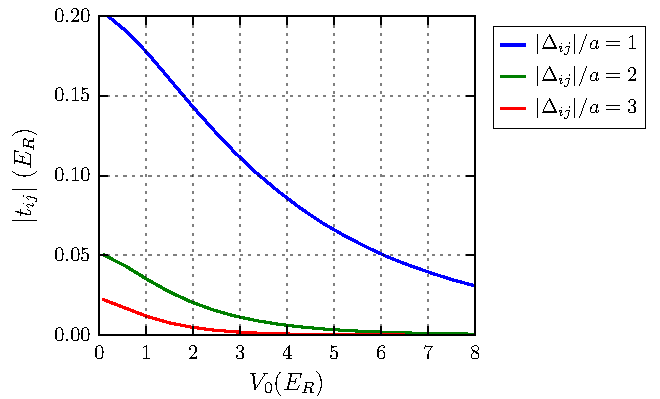
\includegraphics[width=0.6\textwidth]{../figures/BandStructure_figures/tightbinding_V0_interp.pdf}
\caption[Tunneling matrix elements in a 3D lattice.]{\small Tunneling matrix
element in an optical lattice as a function of lattice depth.  Nearest-neighbor
and beyond nearest-neighbor matrix elements are shown to illustrate the range
of lattice depths for which the tight-binding limit is a good approximation.
$\Delta_{ij}$ corresponds to the distance between initial and final lattice
sites in the tunneling matrix element.  For $V_{0}\gtrsim 5\,E_{r}$ we can
safely neglect tunneling beyond nearest neighbors.  } \label{fig:tightbinding}
\end{figure}

Yet another way of estimating the tunneling matrix element \cite{Bloch2008} is
by using the relationship $t=W_{\text{1D}}/4$, valid in the tight-binding
limit, and then working backwards.  An analytical form for the bandwidth can be
obtained from the known properties of the Mathieu functions, which are
solutions to the Schrodinger equation in a 1D lattice.  This approach yields
the analytic result 
\begin{equation}
 t/\er \simeq \frac{4}{\sqrt{\pi}} \vvo^{3/4} \exp(-2\sqrt{\vvo}) 
\label{eq:tunnelMathieu}
\end{equation} 
where \vvo\ is the lattice depth in units of the recoil energy. This formula
appears in a popular review of the subject~\cite{Bloch2008} and is thus widely
used.  The comparison between the result from Eq.~\ref{eq:tunneling3D} and
Eq.~\ref{eq:tunnelMathieu} is shown in Fig.~\ref{fig:tMathieu}. 
\begin{figure}
\centering
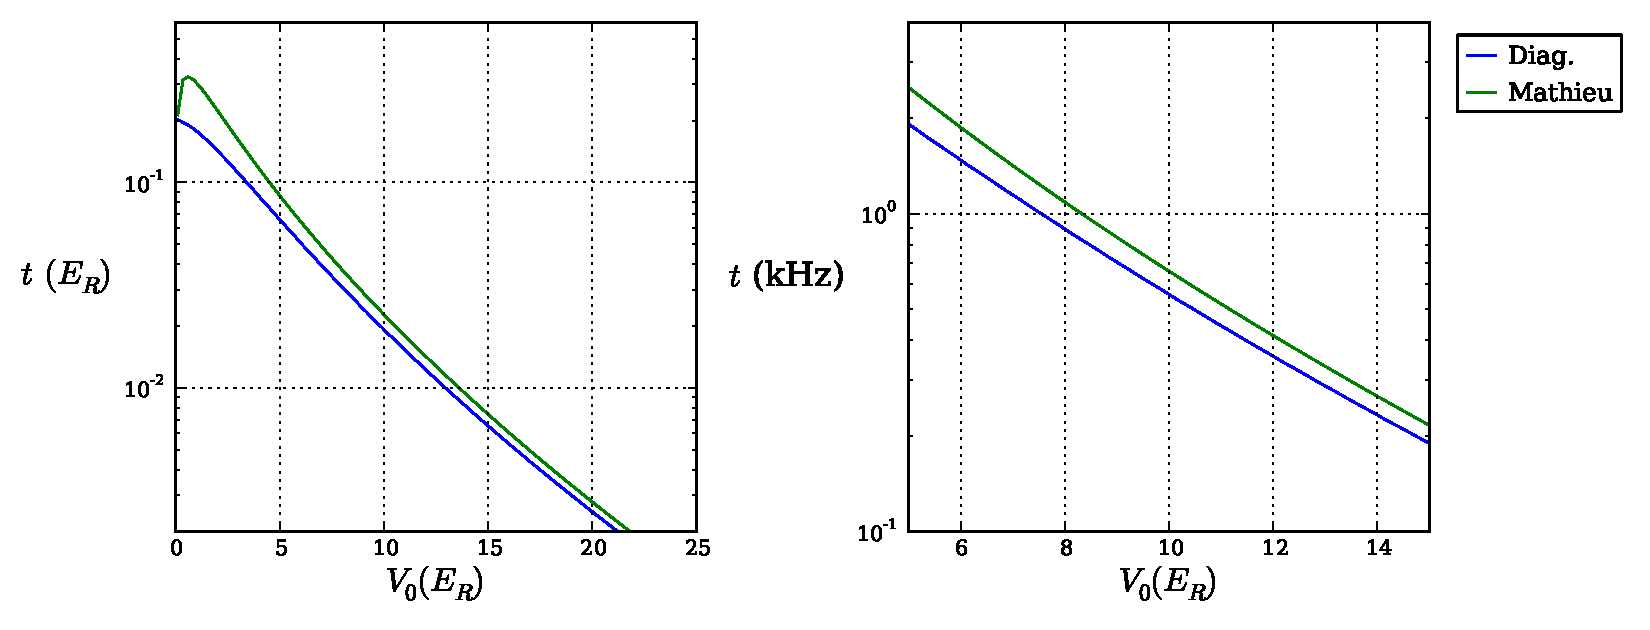
\includegraphics[width=\textwidth]{../figures/BandStructure_figures/tunneling_V0_Mathieu.pdf}
\caption[Nearest neighbor tunneling matrix element]{\small Nearest neighbor
tunneling matrix element in an optical lattice as a function of lattice depth.
Comparison between the result from Eq.~\ref{eq:tunneling3D} (blue line) and the
one obtained from the Mathieu functions, Eq.~\ref{eq:tunnelMathieu} (green
line).  The right panel shows the tunneling rate in kHz for the mass of a
$^{6}$Li atom.  At 7\,$E_{r}$, where we perform most of our experiments, the
discrepancy can be significant.  }
\label{fig:tMathieu}
\end{figure}

%Finally, we have the second quantized form of $H_{0}$ in the tight-binding
%limit 
%\begin{equation}
%  H_{0} = -t \sum_{ \langle ij \rangle } a_{i}^{\dagger}a_{j} 
%\end{equation}
%where the $\langle \rangle$ denote nearest-neighbors, and the creation operator
%$a_{i}^{\dagger}$ create particles in the Wannier state localized at site $i$.

Notice that, up to now, we have ignored the spin part of the wavefunction.   We
can include it easily by noticing that $H_{0}$ does not act on the spin at all,
so the states $|i\rangle$ and $|j\rangle$ that we have used in the derivation
above need to have the same spin.   If two spin states are available, our basis
set is twice as large, which can be taken care of by including a sum over spin
states in the second quantized form of the Hamiltonian:
\begin{equation}
  H_{0} = \bar{E}\sum_{i}  a_{i}^{\dagger} a_{i} \, -\ t
   \!\!\! 
  \sum_{ \langle ij \rangle, \sigma=\dbl   } 
   \!\!\!
  a_{i\sigma}^{\dagger}a_{j\sigma} 
\end{equation}

\paragraph{On-site interaction energy, $\bm{U}$.}

The interaction part of the Hamiltonian for $N$ particles is
given by \begin{equation}
    H_{\text{int}} = 
         \frac{1}{2}\sum_{ l,m, l\neq m}^{N} 
         V_{\mathrm{int}}(\bv{r}_{l},\bv{r}_{m} )\\ 
\end{equation}
This is a two-particle operator, and its second quantized form is given by
\begin{equation}
   H_{\text{int}} = \frac{1}{2} \sum_{i,j,k,m} 
           \langle ij | V_{\mathrm{int}} | km \rangle
           a_{i}^{\dagger} a_{j}^{\dagger} a_{m} a_{k}
\end{equation}
where 
\begin{equation}
    \langle ij | V_{\mathrm{int}} | km \rangle =
    \int \mathrm{d}\bv{r}_{1} \int \mathrm{d}\bv{r}_{2} \ \  
    \varphi_{i}^{*}(\bv{r}_{1}) \varphi_{j}^{*}(\bv{r}_{2}) 
    V_{\mathrm{int}}(\bv{r}_{1},\bv{r}_{2}) 
    \varphi_{k}(\bv{r}_{1}) \varphi_{m}(\bv{r}_{2}) 
\end{equation}
and the $\varphi$'s correspond to the wavefunctions of the single particle
basis states chosen. 

The interaction between ultracold atoms can be described in terms of the
$s$-wave scattering length, $a_{s}$,  and a
pseudo-potential~\cite{sakurai2014modern,Bloch2008} given by\footnote{This is a
good approximation as long as the $s$-wave scattering lengths is small compared
to the single-site harmonic oscillator length~\cite{Busch1998}. This condition
is typically satisfied, and other concerns such as collisional losses or
coupling to higher bands become more important well before the $s$-wave
scattering length is comparable to the harmonic oscillator length.  For
reference, the harmonic oscillator length in a lattice site is $\ell = a / (\pi
\vvo^{1/4})$, which for a 7\,\er\ lattice with $a=532\,$nm is $\ell \approx
2000\,a_{0}$, where $a_{0}$ is the Bohr radius.}
\begin{equation}
    V_{\mathrm{int}}(\bv{r}_{1},\bv{r}_{2}) 
    = \frac{ 4 \pi \hbar^{2} a_{s} } { m } \delta(\bv{r}_{1}-\bv{r}_{2}) 
\end{equation}
so the matrix element above can be written as 
\begin{equation}
    \langle ij | V_{\mathrm{int}} | km \rangle =
\frac{ 4 \pi \hbar^{2} a_{s} } { m }
    \int \mathrm{d}\bv{r}  \ \  \varphi_{i}^{*}(\bv{r}) \varphi_{j}^{*}(\bv{r}) 
                                \varphi_{k}(\bv{r}) \varphi_{m}(\bv{r}) 
\end{equation}
Our basis states, $\varphi$, are the 3D Wannier states defined in
Eq.~\ref{eq:wannier3D}, which are separable in the three spatial coordinates.
We recall that the Wannier states are labeled by the lattice site around which
they are centered, and by their band index.   If we explicitly write out the two
labels in the expression above, we obtain
\begin{equation}
    \langle ij | V_{\mathrm{int}} | km \rangle =
\frac{ 4 \pi \hbar^{2} a } { m }
  \prod_{v=x,y,z}
    \int \mathrm{d}v  \ \ 
    w_{i}^{n_{i}}(v) w_{j}^{n_{j}}(v) w_{k}^{n_{k}}(v) w_{m}^{n_{m}}(v) 
   \equiv \, U_{ijkm}
\end{equation}

In general $i,j,k,m$ can represent any lattice sites.  We will restrict
our treatment to on-site interactions by enforcing $i=j=k=m$,  furthermore, we
consider only Wannier states in the lowest band. 
%The Wannier function along  $x,y,z$ depends on the lattice depth along the
%respective coordinate.  We will consider a lattice with different depths along
%the three spatial coordinates, $\bvo = ( V_{0x}, V_{0y}, V_{0z} ) $.  At this
%point we make the approximation of neglecting all of the off-site interaction
%terms, which can be justified by the localized nature of the Wannier states.
%Furthermore, we consider only Wannier states in the lowest band, which is
%valid for scattering lengths smaller than the single-site harmonic oscillator
%length~\cite{Busch1998}.  
With this considerations, and also explicitly writing down the spin quantum
number, we find 
\begin{equation}
   H_{\text{int}} =  
           \frac{U}{2}
        \sum_{i} 
         \left( 
           a_{i\spup}^{\dagger} a_{i\spdn}^{\dagger} a_{i\spdn} a_{i\spup} +
           a_{i\spdn}^{\dagger} a_{i\spup}^{\dagger} a_{i\spup} a_{i\spdn}
         \right)\\
\end{equation}
where we have defined $U\equiv U_{ijkm}$ for $i=j=k=m$, with $U$ is given by  
%\begin{equation}
%  U = 
%  \frac{ 4 \pi \hbar^{2} a } { m }
%   \prod_{v=x,y,z}  \int  w(v) ^{4} \mathrm{d}v  
%\end{equation}
%In units of $E_{R}$, 
\begin{equation}
  U/\er = \frac{ 8}{ \pi}  \frac{ a_{s} }{a}
   \prod_{v=x,y,z}  \int  w(v) ^{4} \mathrm{d}v  
\end{equation}

Defining the number operator as $n_{i\sigma} = a_{i\sigma}^{\dagger}
a_{i\sigma}$ 
\begin{equation}
\begin{split}
   H_{\text{int}}  
     = & \  
           \frac{U}{2}
         \sum_{i} \left( 
           n_{i\spdn} n_{i\spup} + 
           n_{i\spup} n_{i\spdn} \right) 
    \\
     = & \ 
           U\sum_{i}
           n_{i\spup} n_{i\spdn}  
\end{split}
\end{equation}
where $i$ runs over all of the lattice sites.  


To calculate the value of $U$ we use the Wannier states obtained in
Sec.~\ref{sec:1Dlattice}.  Alternatively, one can approximate the Wannier state
by the Gaussian ground state in the local oscillator potential of one lattice
site and carry out the integral analytically to obtain~\cite{Bloch2008} 
\begin{equation} 
  U  = \sqrt{ 8\pi } \frac{a_{s}}{a} \vvo^{3/4} 
\end{equation} 
Figure~\ref{fig:wfactor} shows a comparison of the exact result and the
Gaussian approximation to the Wannier state for a lattice with
$\lambda=1064$\,nm. 
\begin{figure}
\centering
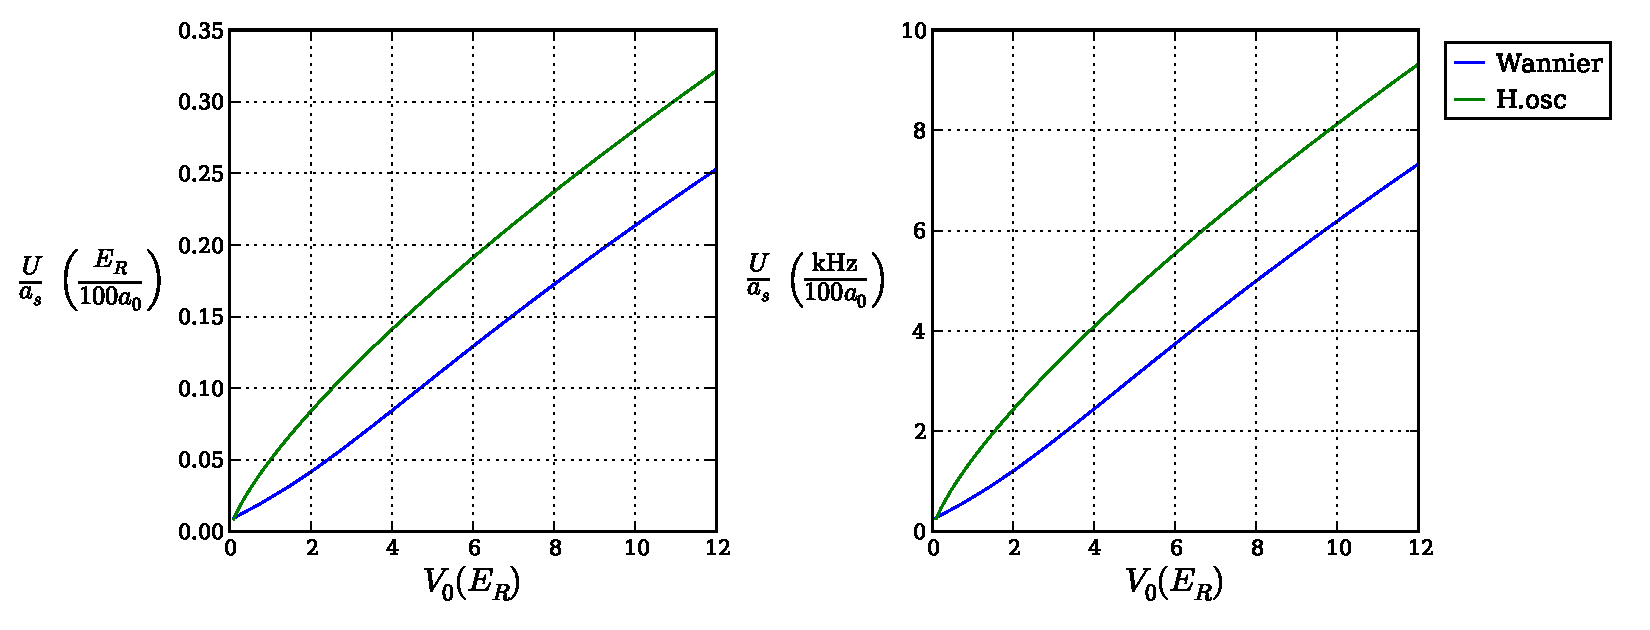
\includegraphics[width=\textwidth]{../figures/BandStructure_figures/wFactor_V0_a0.pdf}
\caption[On-site interactions in a 3D lattice]{\small On-site interactions in a
3D lattice ($\lambda=1064\,\text{nm}$) as a function of lattice depth.
Numerical calculation using Wannier functions (blue line) compared to the
approximation using harmonic oscillator states (green line).  The lattice
depth is the same in all three directions of the lattice.   The left panel
shows uses \er\ for the units of $U$ and the right panel uses kHz for $U/h$. }
\label{fig:wfactor}
\end{figure}

If the on-site interaction term is comparable to the energy spacing between the
lowest and first excited bands, the single band approximation presented here
breaks down.  Corrections to the tunneling rate and the on-site interactions
are necessary, which may depend on the lattice site
occupation~\cite{Werner2005,Jordens2010,Mark2012}.

\section{Parameter regimes for a valid description using a single band
Hubbard model}

Throughout this chapter we have mentioned the possible scenarios for which the
single band Hubbard model is not an accurate description of ultracold atoms in
an optical lattice.  The two most important ones are:
\begin{itemize} 
\item The on-site interaction $U$ is comparable to the band gap $\Delta$.  The
band gap is the energy difference between the highest energy state in the
lowest band and the lowest energy state in the first excited band, see
Fig.~\ref{fig:bands3d_V0}. \item Tunneling beyond nearest-neighbor (rate
$t_{2}\equiv t_{ij}$ for $\Delta_{ij}=2a$, see Fig.~\ref{fig:tightbinding}) is
not negligible compared to nearest-neighbor tunneling (rate $t$), i.e.  the
tight-binding approximation does not hold. 
\end{itemize}
In Fig.~\ref{fig:hubbardvalid} we have represented these two conditions as a
function of the lattice depth and the $s$-wave scattering length.  For more
details on the validity of the single band Hubbard Hamiltonian see
Ref.~\cite{Werner2005}. 
\begin{figure}
\centering
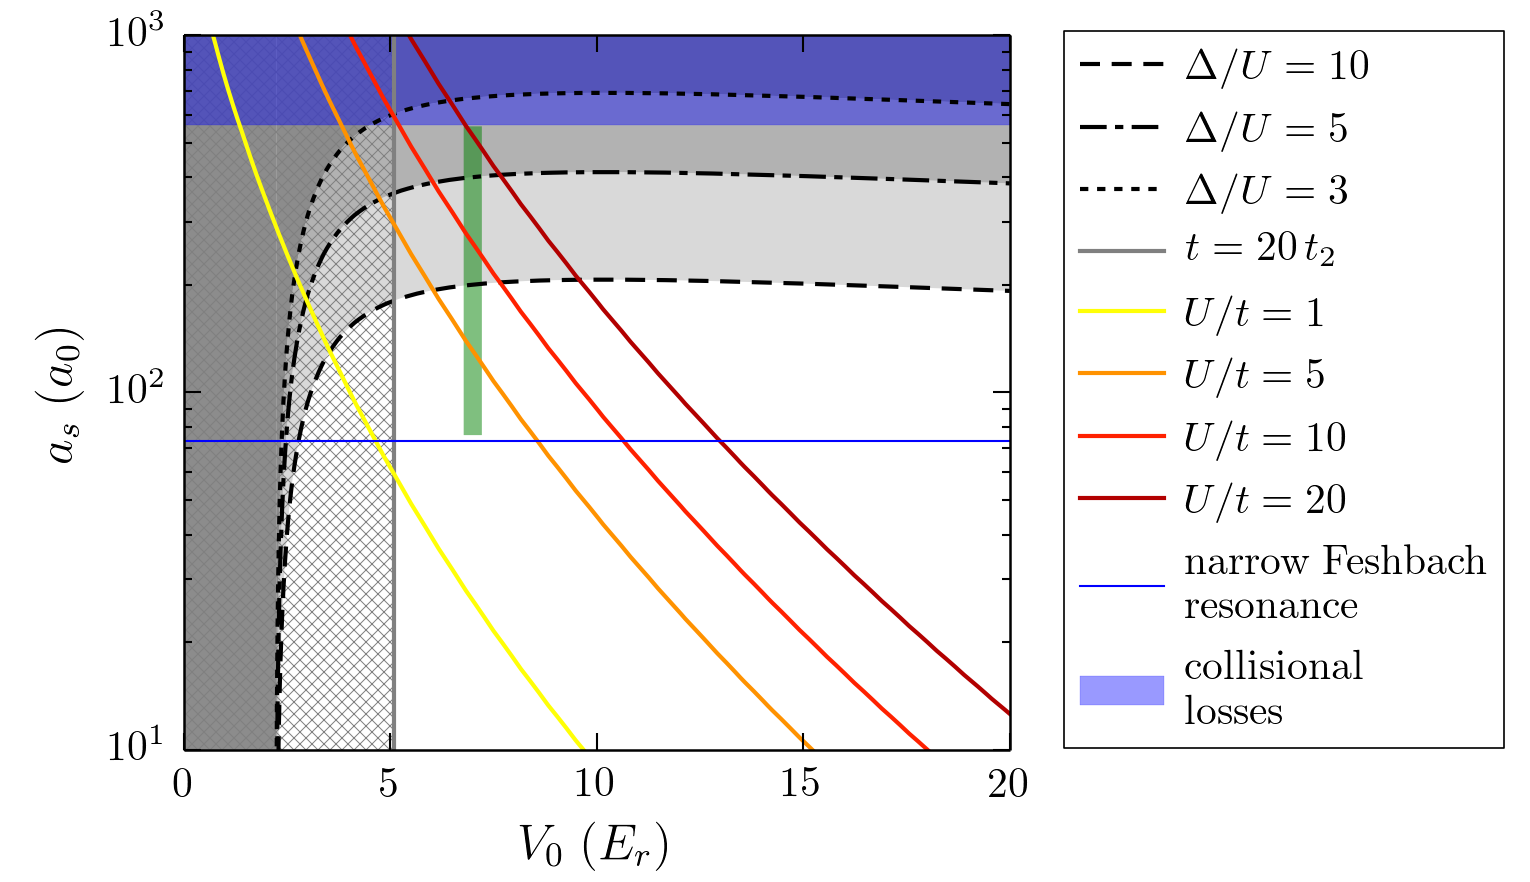
\includegraphics[width=0.9\textwidth]{../figures/BandStructure_figures/singleband.png}
\caption[Regimes of validity for the single band Hubbard Hamiltonian]{\small
Regimes of validity for the single band Hubbard Hamiltonian.   The dashed black
lines show curves at constant $\Delta/U$.  As $U$ approaches $\Delta$, higher
bands have to be taken into account to describe the system
accurately~\cite{Werner2005}.  The vertical gray line indicates the lattice
depth at which $t = 20t_{2}$, which delimits the region of validity of the
tight-binding approximation.  Yellow to brown hued lines indicated curves at
constant $U/t$.  The thin blue line indicates the background $s$-wave
scattering length in the vicinity of the narrow Feshbach resonance of
$^{6}Li$~\cite{Strecker2003,Zurn2013}.  The shaded blue area indicates the
range of scattering lengths over which we see significant collisional losses
and heating of the sample.   The shaded green area denotes the parameter regime
covered by the experiments carried out in this thesis.} 
\label{fig:hubbardvalid}
\end{figure}


 
%%%%%%%%%%%%%%%%%%%%%%%%%%%%%%%%%%%%%%%%%%%%%%%%%%%%%%%%%%%%%%%%%%%%%%%%%%%%%%%
%%%%%%%%%%%%%%%%%%%%%%%%%%%%%%%%%%%%%%%%%%%%%%%%%%%%%%%%%%%%%%%%%%%%%%%%%%%%%%%
%%%%  CHAPTER 3 
%%%%%%%%%%%%%%%%%%%%%%%%%%%%%%%%%%%%%%%%%%%%%%%%%%%%%%%%%%%%%%%%%%%%%%%%%%%%%%%
%%%%%%%%%%%%%%%%%%%%%%%%%%%%%%%%%%%%%%%%%%%%%%%%%%%%%%%%%%%%%%%%%%%%%%%%%%%%%%%
\chapter{The Hubbard model}
\label{chap:hubbardmodel}

In Chapter 2 we saw how ultracold atoms, under a large range of values for the
lattice depth and the $s$-wave scattering length are a nearly ideal realization
of the single band Hubbard model.   The Hubbard model, nevertheless, was not
originally formulated with these kind of systems in mind; it originated as an
overly simplified picture for the description of electrons in solids.   In this
chapter we start by providing a brief historical perspective of the Hubbard
model.  We then go on to introduce simplified treatments of the model which
will allow us to gain insight into its physics. We conclude by describing some
of the latest advances in numerical simulations. 

\section{A bit of history}

%The contents of this section are based on the book ``Out of the Crystal
%Maze''~\cite{hoddeson1992out}, which chronicles the origin and development of
%solid state physics from 1920 to 1960. 

% References: 
%
% Louis Neel Nobel Lecture
% Out of the Crystal Maze
% Magnetism in condensed matter  
% Hubbard's original paper. 

At the end of the 1920's, when the foundations of quantum mechanics were almost
all formally laid out, there were quite a few phenomena begging for a touch of
quantum mechanics to elucidate the physics behind them.  One of those problems
was ferromagnetism.    Ferromagnetism was first understood classically within
the Weiss picture of a molecular field,   in which a ferromagnet is treated as
a paramagnet under the influence of a fictitious magnetic field (the molecular
field), which is postulated to be proportional to the magnetization.  It was
Heisenberg in 1928~\cite{Heisenberg:1928:TFG} who realized that the exchange
interaction, as used by Heitler and London to explain the singlet and triplet
energy level splitting of the Helium atom, was responsible for the existence
and magnitude of Weiss's molecular field.   This motivated the Heisenberg model for ferromagnetism 
\begin{equation}
   H = -\sum_{ij} J_{ij} \bv{S}_{i} \cdot \bv{S}_{j} 
\end{equation} 
where $J_{ij}$ is the exchange constant between spins  that are localized at
sites  $i$  and $j$ in a crystal lattice.  Under the assumption that only
nearest neighboring spins affect each other, the Heisenberg model can account
for the Curie temperature of ferromagnets, with reasonable values of $J$ as an
input.  However, even though Heisenberg's theory of ferromagnetism had the
correct physical basis, a formal calculation of the exchange term, $J$, for a
large system of interacting electrons is too difficult to carry out.  

% Further work by
%Bloch, Slater, Bethe and others led to further understanding of the
%ferromagnetic state, such as the discovery of spin waves.  However, the problem
%remained a challenge, primarily due to the interactions between electrons.  


%Around the same time as Heisenberg developed his theory of ferromagnetism,  his
%Ph.D student Felix Bloch established the theory of energy bands (tight-binding
%model) to describe the behavior of conduction electrons in
%solids~\cite{Bloch1929lattice}.    
%At the time there was some dissatisfaction
%with the work of Heisenberg, because even though it had the correct physical
%basis, a formal calculation of the exchange term for a large system of
%interacting electrons proved too difficult to carry out.  With iron being a
%ferromagnetic metal, the role that the $s$ conduction electrons could be
%playing in its ferromagnetic properties (for instance the interaction of $d$
%electrons with $s$ electrons)  was an important question, which Bloch set out
%to answer using his band theory as a starting point.   Bloch realized that the
%exchange term could sometimes have a negative sign, which would not be
%consistent with ferromagnetism.  He came to the conclusion that, only for
%narrow energy bands (which favor wavefunctions that are more localized around
%the atoms), would the exchange interaction produce a ferromagnetic state.   Bloch was unable to 
%
% Pauli paramagnetism ( magnetism of the spins ) 
% Landau diagmagnetism ( magnetism of the free electrons being charged 
% particles and quantized Landau levels in B field)

%By the early 1930's, the band theory of solids, developed by Bloch during his
%PhD in 1928~\cite{Bloch1929lattice},  had become the foundation of solid state
%physics. In the following years, the interest in the field began to shift from
%general principles to computation of the properties of particular materials.
%Nevertheless, 

The problem of $d$ electrons in ferromagnetic metals  was still of much
interest in the early 1960's.    A lot of attention had been given in the
previous decade to the issue of considering the consequences of interactions
between electrons (correlations) in a free electron gas.  This was very
important for the description of electrons in conduction bands, but not
satisfactory when considering partially filled $d$ or $f$ bands, such as those
present in the transition and rare-earth metals.    In particular, the $d$
electrons of the transition metals  were of major interest at the time because
they are not as localized as $f$ electrons, but also not as ``free'' as
$s$-electrons in a conduction band.  

Hubbard realized, in the early 60's, that the problem of $d$-electrons could be
thought of as a problem of electrons in a conduction band, where the effects of
interactions between electrons (correlations) give rise to behavior more
consistent with an atomic picture of localized electrons. He then postulated a
model~\cite{Hubbard26111963}, now known as the Hubbard model,  as an extension
of the tight-binding model (the simplest model for an energy band) on which the
effects of correlations are simplified at maximum without removing them
altogether.   The hope was to see the behavior of electrons as localized
moments, i.e. ferromagnetism or an insulating state, emerge solely as a
consequence of electron correlations in a conduction band. 

To simplify the role of correlations, Hubbard neglected all of the terms due to
interactions, except the one where two electrons are on the same site.  As we
saw in Chapter~2, this approximation is easy to express in the second quantized
formalism using Wannier states as a single particle basis.  The on-site
interaction term for the Coulomb energy between two electrons is then:
\begin{equation}
U =  \int 
      w^{*}( \bv{x} - \bv{R}_{i} )
      w( \bv{x} - \bv{R}_{k} )
 \left( \frac{ e^{2} }{ | \bv{x} - \bv{x}' | } \right) 
      w^{*}( \bv{x}' - \bv{R}_{j} )
      w( \bv{x}' - \bv{R}_{l} )
 \ \mathrm{d}\bv{x}\mathrm{d}\bv{x}'
\end{equation}
where $w$ are the Wannier states, introduced in Chapter~2, and $\bv{R}_{i} =
\bv{R}_{j} = \bv{R}_{k} = \bv{R}_{l}$.  In the same year as Hubbard,
Gutzwiller~\cite{PhysRevLett.10.159} and Kanamori~\cite{Kanamori01091963},
independently formulated essentially the same model for $d$ electrons. 

Another thing to point out about the Hubbard model is that even though it was
conceived with the problem of $d$-electrons in mind, the band considered in the
model is an $s$-band. In a $d$-band there are 10 different levels that an
electron can occupy, however in an $s$-band there are only two, spin up and
spin down.  Hubbard himself commented on this point and said: ``one may
nevertheless hope to obtain some results of general
application''~\cite{Hubbard26111963},.  

%In 1936 Louis N\'{e}el noted that, since the exchange energy originates from
%short range overlap between wavefunctions, then it would be possible for it to
%give rise to an antiferromagnetic state.   An antiferromagnetic state can form
%in a bipartite lattice,  a lattice that can be subdivided into two sublattices
%such that for any given site all of its neighbors belong to the other
%sublattice.   For a system with a negative value of the exchange integral then
%the antiferroma 

\section{Hubbard model for a single lattice site, $t=0$}

%For a more complete introduction to the Hubbard model refer to
%Ref.~\cite{Scalettar:hubbard7}. 

In the Hubbard model, the limit of no interactions,  $U=0$, takes us simply
back to the tight-binding model.  In this case the properties of the system can
be well understood in terms of a single particle picture, where electrons
occupy the single particle energy levels of the Hamiltonian according to the
Fermi-Dirac distribution.  The dispersion relation of the tight-binding model
determines the density of states, and the thermodynamics at low temperature can
be obtained from the value of the Fermi energy and the temperature by making
use of Sommerfeld's approach for approximating Fermi-Dirac
integrals~\cite{ashcroft1976solid}.

On the other hand, the limit of no tunneling~\cite{Scalettar:hubbard7}, $t=0$,
will allow us to gain some insight into the thermodynamics of the Hubbard
model.  In this case the lattice sites can be considered to be completely
independent of each other, and the partition function of the total system is
simply a product of the partition function for a system with a single lattice
site.

We recall the Hubbard Hamiltonian:
\begin{equation}
  H =  
-t \sum_{ \langle ij \rangle, \sigma   } 
          a_{i\sigma}^{\dagger}a_{j\sigma} 
         + U\sum_{i} n_{i\spup} n_{i\spdn}  
   - \mu \sum_{i}  ( n_{i\spup} + n_{i\spdn} ) 
\end{equation}
where $\mu$ is the chemical potential, and the term $- \mu \sum_{i}  (
n_{i\spup} + n_{i\spdn} ) $ is included to work in the grand
canonical ensemble, where the particle number is allowed to vary. 

The grand canonical partition function is given by
\begin{equation} 
 Z = \text{Tr} e^{-\beta H}  =  z^{N} 
\end{equation} 
where $z$ is the partition function for an individual site given by
\begin{equation}
  z = 1 + 2e^{\beta\mu} + e^{2\beta\mu - \beta U} 
\end{equation}
With the partition function in hand we can obtain the thermodynamic quantities
as derivatives of the grand canonical potential, $\Omega = - \ln Z /
\beta $.  We have for the density, double occupancy, and entropy per lattice
site:
\begin{equation}
  n  = -\frac{1}{N}\frac{\partial \Omega}{ \partial \mu } ~~~~~~~~~
  d  = \frac{1}{N}\frac{\partial \Omega}{ \partial U }  ~~~~~~~~~
  s  = -\frac{1}{N}\frac{\partial \Omega}{ \partial T} 
\end{equation}

For example, the explicit expression for the density can be derived:
\begin{equation}
  n  = 2\frac{ e^{\beta \mu} + e^{2\beta\mu - \beta U} }
          { 1 + 2e^{\beta \mu} + e^{2\beta\mu-\beta U } } 
\end{equation}
An important physical quantity in the Hubbard model is the local moment,
defined as 
\begin{equation}
  \langle m ^{2} \rangle = \langle ( n_{\spup} - n_{\spdn} )^{2} \rangle  = n - 2d 
\end{equation} 
If there is no probability of having doubly occupied sites, $d=0$ and the local
moment simply becomes equal to the density $n$.   From the grand potential we
obtain the expression
\begin{equation} 
  \langle m ^{2} \rangle =  2\frac{ e^{\beta \mu}  }
          { 1 + 2e^{\beta \mu} + e^{2\beta\mu-\beta U } } 
\end{equation}
 
In Fig.~\ref{fig:0t_occupation} we show plots of the density and the local
moment versus chemical potential for various temperatures.  As we mentioned
above, the Hubbard model describes an $s$-band with a maximum capacity of two
electrons per lattice site.   When the average number of particles per site in
the Hubbard model  is $n=1$, the system is said to be at half-filling.
Figure~\ref{fig:0t_occupation} shows us that there is a plateau in the density
as a function of chemical potential which occurs at half-filling for
sufficiently low temperatures.   This plateau is an indication of the Mott
insulating gap, it can be interpreted as a discontinuous jump in the energy
necessary to add an extra particle to the system.   At the same time we see
that the local moment goes to 1, equal to the density at half filling, which
tells us that in the Mott insulating plateau the probability of finding doubly
occupied sites goes to zero, as well as the fluctuations in the number of
particles per site 
\begin{figure}
\centering
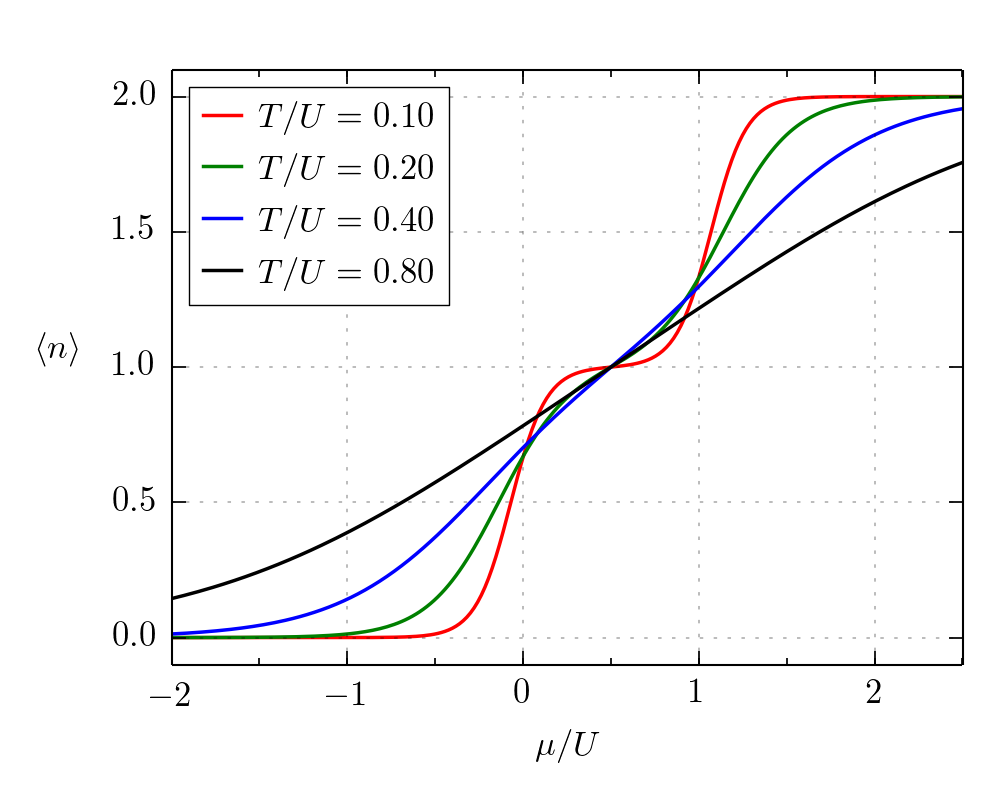
\includegraphics[width=0.48\textwidth]{../figures/hubbard/hubbard_0t_occupation.png}
~
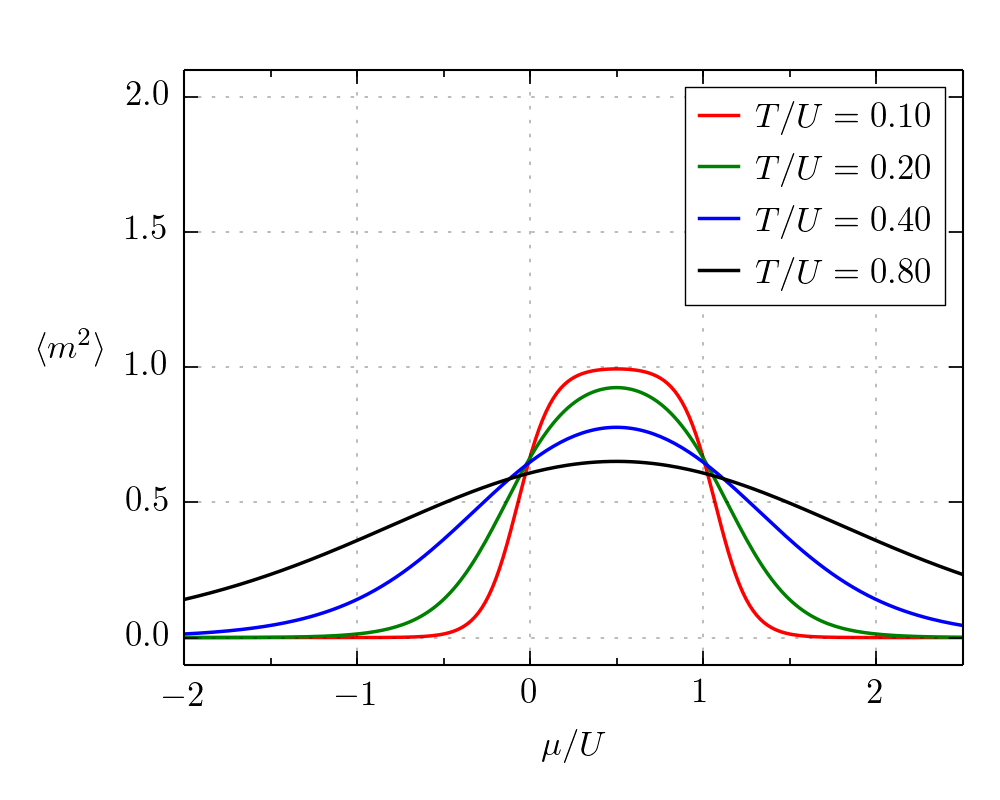
\includegraphics[width=0.48\textwidth]{../figures/hubbard/hubbard_0t_moments.png}
\caption[Density and local moment in the Hubbard model at $t=0$]{\small Density
and local moment versus chemical potential in the Hubbard model for $t=0$.  In
this limit the Hubbard model represents a collection of uncorrelated lattice
sites.  For a temperature, $T$, significantly lower than the on-site
interaction, $U$,  the density shows a plateau as a function of chemical
potential, representative of the Mott insulating gap. At the same time the
local moment goes to 1, indicating the absence of doubly occupied sites, and
the suppression of fluctuations on the number of atoms per site, two indicators
of an insulating state.  } 
\label{fig:0t_occupation}
\end{figure}

In the previous paragraph we suggested that the plateau in $n$ vs. $\mu$ is
indicative of an energy gap.  In more formal terms, to establish the presence
of a gap in the spectrum of a many-body system, one should calculate the
pseudo-particle density of states (also known as the spectral function).  This
was done by Hubbard on the third of the series of papers that followed his
introduction of the Hubbard model~\cite{Hubbard1964}, and he showed that his
model predicted the  existence of the Mott-Hubbard insulating gap.  In 1949,
Mott had suggested that the Coulomb interaction was responsible for the
insulating properties of nickel monoxide (NiO), a material with a partially
filled band that should be a conductor according to conventional band
theory~\cite{Mott1949}.  The treatment by Hubbard was the first formal
treatment of the Mott metal-insulator transition~\cite{RevModPhys.40.677} and
the first big success of the Hubbard model.


\section{Particle-hole symmetry} 

The reader may have noticed, by looking at Fig.~\ref{fig:0t_occupation}, that
all of the plotted curves have a symmetry about $\mu=U/2$.    All of the the
thermodynamic properties of the Hubbard model exhibit this symmetry, a
consequence of the particle-hole symmetry of the Hamiltonian,  and one only
needs to obtain them for densities $0\leq n \leq 1$, as they can be inferred
for $1\leq n \leq 2$ by reflection about $\mu=U/2$.  In some theoretical
treatments it is desirable to have the reflection point be independent of $U$,
so a shift is introduced in the chemical potential $\mu' = \mu-U/2$ which
results in the ``particle-hole symmetric'' form of the Hubbard Hamiltonian:
\begin{equation}
  H' =  
-t \sum_{ \langle ij \rangle, \sigma   } 
          a_{i\sigma}^{\dagger}a_{j\sigma} 
         + U\sum_{i} \left( n_{i\spup} -\frac{1}{2}\right) 
                     \left( n_{i\spdn} -\frac{1}{2}\right) 
   - \mu' \sum_{i}  ( n_{i\spup} + n_{i\spdn} ) 
\end{equation}
This form produces the same physical results as the non-shifted one. 
 

\section{Exact diagonalization} 

The treatment of the single-site limit of the Hubbard model was very simple and
we showed how to obtain an expression for the grand potential, from which all of
the thermodynamic properties can be obtained.  From this simple treatment we
saw how the Mott insulating gap opens up at low temperatures, and a Mott
insulator, with exactly one particle per lattice site, can exist at
half-filling.   At even lower temperatures it is well known that the localized
moments of the Mott insulator order themselves into an AFM ordered state. 

In what follows we will obtain the exact solution for the ground state of
models with 2 sites and 4 sites.  These solutions are going to motivate the
antiferromagnetic character of the ground state of the Hubbard model, and give
us a glimpse of the connection between the Hubbard model and high-$T_{c}$
superconductivity. 

\subsubsection { Exact diagonalization for 2 sites } 

The full Hilbert space for a two-site model has dimension 16.  To do an exact
diagonalization we will restrict to a sector at half-filling with a balanced
spin-mixture (equal number of up and down spins).  The basis states are:
\begin{align}
  |\ndbl, \nvac \rangle  & =  
      a_{1\spup}^{\dagger} a_{1\spdn}^{\dagger} |\nvac\rangle \\  
  |\nspdn, \nspup \rangle & =    
      a_{1\spdn}^{\dagger} a_{2\spup}^{\dagger} |\nvac\rangle \\  
  |\nspup, \nspdn \rangle & =   
      a_{1\spup}^{\dagger} a_{2\spdn}^{\dagger} |\nvac\rangle \\  
  | \nvac, \ndbl \rangle & =  
      a_{2\spup}^{\dagger} a_{2\spdn}^{\dagger} |\nvac\rangle \\  
\end{align}
Notice that we have chosen the ordering convention for fermion creation
operators in which lower site indices are leftmost and spin up is to the left
of spin down.   Calculating the matrix elements of the Hubbard Hamiltonian in
this basis is an exercise in tracking minus signs when commuting fermion
creation and annihilation operators.   We have automated that procedure by
writing a python program which is available online~\cite{PedroMDuarte:11558}.

The resulting matrix for the Hamiltonian is 
\begin{equation}
H =   
\left(
\begin{array}{cccc}
 U & 0 & -t & -t \\
 0 & U & -t & -t \\
 -t & -t & 0 & 0 \\
 -t & -t & 0 & 0 \\
\end{array}
\right)  
\end{equation}
which can be analytically diagonalized to obtain the eigenvalues
\begin{equation}
\begin{array}{c}
 \frac{1}{2} \left(U-\sqrt{16 t^2+U^2}\right) \\
 0 \\
 U \\
 \frac{1}{2} \left(U+\sqrt{16 t^2+U^2}\right) \\
\end{array}
\end{equation}
For large $U/t$ the energy of the ground state goes to $\approx -4 t^{2}/U$,
which is the value of the AFM exchange energy.  In Fig.~\ref{fig:exact_2site}
we show plots of the energy eigenvalues as a function of $U/t$ and also show
the composition of the energy eigenstates in terms of our basis states.  
\begin{figure}
\centering
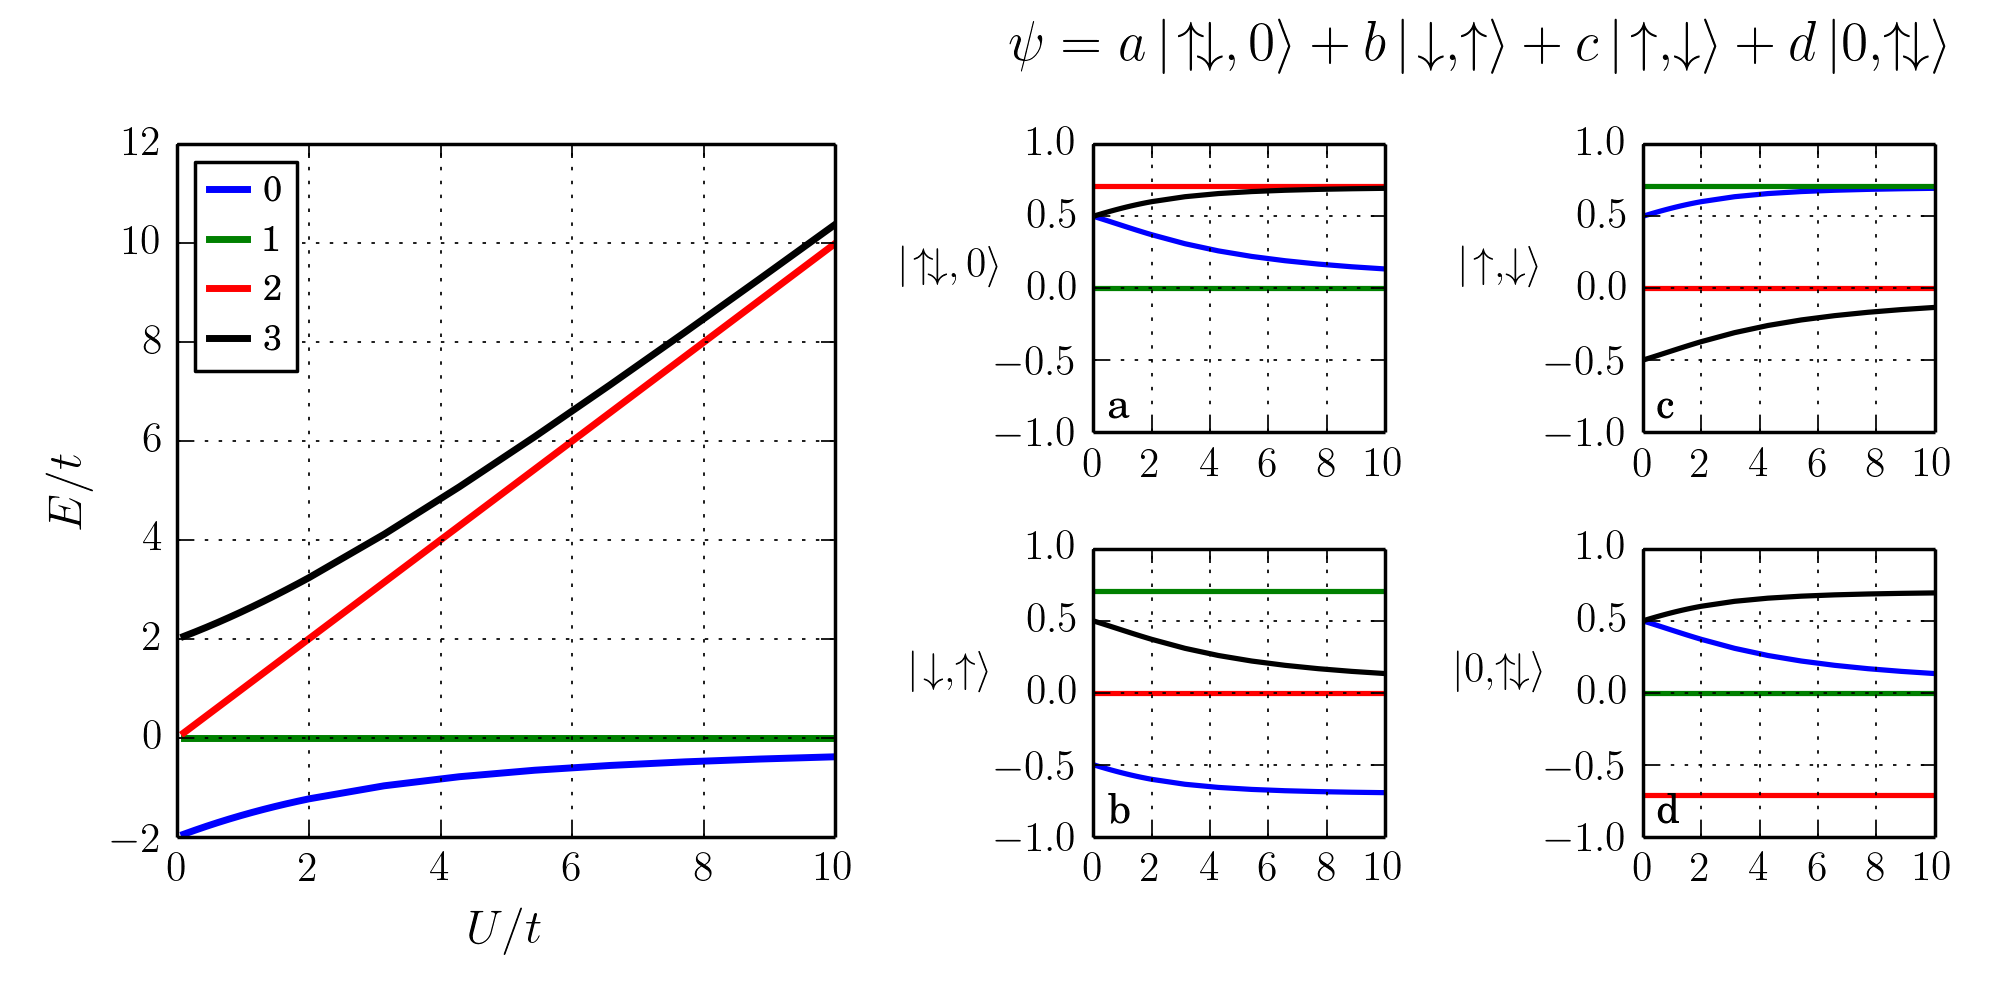
\includegraphics[width=0.7\textwidth]{../figures/hubbard/Ut_eigenvalues_2site.png}
\caption[Exact diagonalization results for two lattice sites.]{\small Energy
eigenvalues and eigenstates for a two lattice site system.  The coefficients
$a,b,c,d$, which define the energy eigenstates are shown in the four panels at
the right.  We see that the ground state has an antiferromagnetic character. } 
\label{fig:exact_2site}
\end{figure}
In the two-site system, we can see the opening of the Mott-Hubbard gap in the
spectrum as $U/t$ is increased, in agreement with the single site treatment.
We can now also see the antiferromagnetic character of the ground state.  In
the limit of large $U/t$, the ground state is given by 
\begin{equation}
    \frac{1}{\sqrt{2}} | \nspup, \nspdn\rangle  
  - \frac{1}{\sqrt{2}} | \nspdn, \nspup\rangle 
\end{equation} 


\subsubsection { Exact diagonalization for 4 sites } 

In the case of four lattice sites (a $2\times$2 plaquette), the basis set in the
half-filling spin-balanced sector grows to contain 36 states.   The Hamiltonian
matrix is a 36$\times$36 matrix, which can be readily diagonalized numerically.
% TO SEE THE MATRIX FOR THE 2X2 PROBLEM UNCOMMENT BELOW
%\begin{equation} \tiny \arraycolsep=1.0pt\def\arraystretch{0.6} \left(
%\begin{array}{cccccccccccccccccccccccccccccccccccc} 2 U & 0 & -t & 0 & t & 0 &
%0 & 0 & 0 & -t & 0 & 0 & 0 & 0 & 0 & 0 & 0 & 0 & t & 0 & 0 & 0 & 0 & 0 & 0 & 0
%& 0 & 0 & 0 & 0 & 0 & 0 & 0 & 0 & 0 & 0 \\ 0 & U & -t & 0 & 0 & 0 & 0 & t & 0
%& t & 0 & 0 & 0 & 0 & 0 & 0 & 0 & 0 & 0 & 0 & -t & 0 & 0 & 0 & 0 & 0 & 0 & 0 &
%0 & 0 & 0 & 0 & 0 & 0 & 0 & 0 \\ -t & -t & U & 0 & 0 & 0 & 0 & 0 & -t & 0 & t
%& t & 0 & 0 & 0 & 0 & 0 & 0 & 0 & 0 & 0 & -t & 0 & 0 & 0 & 0 & 0 & 0 & 0 & 0 &
%0 & 0 & 0 & 0 & 0 & 0 \\ 0 & 0 & 0 & U & -t & 0 & t & 0 & 0 & 0 & 0 & 0 & -t &
%0 & 0 & 0 & 0 & 0 & t & 0 & 0 & 0 & 0 & 0 & 0 & 0 & 0 & 0 & 0 & 0 & 0 & 0 & 0
%& 0 & 0 & 0 \\ t & 0 & 0 & -t & U & 0 & 0 & 0 & t & 0 & 0 & 0 & 0 & 0 & t & 0
%& 0 & 0 & 0 & t & 0 & 0 & 0 & 0 & -t & 0 & 0 & 0 & 0 & 0 & 0 & 0 & 0 & 0 & 0 &
%0 \\ 0 & 0 & 0 & 0 & 0 & 2 U & -t & t & 0 & 0 & 0 & 0 & -t & 0 & 0 & 0 & 0 & 0
%& 0 & 0 & t & 0 & 0 & 0 & 0 & 0 & 0 & 0 & 0 & 0 & 0 & 0 & 0 & 0 & 0 & 0 \\ 0 &
%0 & 0 & t & 0 & -t & U & 0 & -t & 0 & 0 & 0 & 0 & -t & 0 & 0 & t & 0 & 0 & 0 &
%0 & t & 0 & 0 & 0 & 0 & 0 & 0 & 0 & 0 & 0 & 0 & 0 & 0 & 0 & 0 \\ 0 & t & 0 & 0
%& 0 & t & 0 & U & t & 0 & 0 & 0 & 0 & 0 & -t & 0 & 0 & 0 & 0 & 0 & 0 & 0 & t &
%0 & 0 & t & 0 & 0 & 0 & 0 & 0 & 0 & 0 & 0 & 0 & 0 \\ 0 & 0 & -t & 0 & t & 0 &
%-t & t & 2 U & 0 & 0 & 0 & 0 & 0 & 0 & -t & 0 & -t & 0 & 0 & 0 & 0 & 0 & t & 0
%& 0 & t & 0 & 0 & 0 & 0 & 0 & 0 & 0 & 0 & 0 \\ -t & t & 0 & 0 & 0 & 0 & 0 & 0
%& 0 & U & -t & t & 0 & 0 & -t & 0 & 0 & 0 & 0 & 0 & 0 & 0 & 0 & 0 & 0 & 0 & 0
%& -t & 0 & 0 & 0 & 0 & 0 & 0 & 0 & 0 \\ 0 & 0 & t & 0 & 0 & 0 & 0 & 0 & 0 & -t
%& U & 0 & 0 & 0 & 0 & t & 0 & 0 & 0 & 0 & 0 & 0 & 0 & 0 & 0 & 0 & 0 & 0 & -t &
%0 & 0 & 0 & 0 & 0 & 0 & 0 \\ 0 & 0 & t & 0 & 0 & 0 & 0 & 0 & 0 & t & 0 & 0 & 0
%& 0 & 0 & 0 & 0 & t & 0 & 0 & 0 & 0 & 0 & 0 & 0 & 0 & 0 & 0 & 0 & 0 & 0 & t &
%0 & 0 & 0 & 0 \\ 0 & 0 & 0 & -t & 0 & -t & 0 & 0 & 0 & 0 & 0 & 0 & U & -t & t
%& 0 & -t & 0 & 0 & 0 & 0 & 0 & 0 & 0 & 0 & 0 & 0 & -t & 0 & 0 & 0 & 0 & 0 & 0
%& 0 & 0 \\ 0 & 0 & 0 & 0 & 0 & 0 & -t & 0 & 0 & 0 & 0 & 0 & -t & 0 & 0 & -t &
%0 & 0 & 0 & 0 & 0 & 0 & 0 & 0 & 0 & 0 & 0 & 0 & -t & 0 & 0 & 0 & 0 & 0 & 0 & 0
%\\ 0 & 0 & 0 & 0 & t & 0 & 0 & -t & 0 & -t & 0 & 0 & t & 0 & 0 & t & 0 & -t &
%0 & 0 & 0 & 0 & 0 & 0 & 0 & 0 & 0 & 0 & 0 & -t & 0 & 0 & 0 & t & 0 & 0 \\ 0 &
%0 & 0 & 0 & 0 & 0 & 0 & 0 & -t & 0 & t & 0 & 0 & -t & t & U & 0 & 0 & 0 & 0 &
%0 & 0 & 0 & 0 & 0 & 0 & 0 & 0 & 0 & 0 & -t & 0 & 0 & 0 & t & 0 \\ 0 & 0 & 0 &
%0 & 0 & 0 & t & 0 & 0 & 0 & 0 & 0 & -t & 0 & 0 & 0 & U & t & 0 & 0 & 0 & 0 & 0
%& 0 & 0 & 0 & 0 & 0 & 0 & 0 & 0 & -t & 0 & 0 & 0 & 0 \\ 0 & 0 & 0 & 0 & 0 & 0
%& 0 & 0 & -t & 0 & 0 & t & 0 & 0 & -t & 0 & t & U & 0 & 0 & 0 & 0 & 0 & 0 & 0
%& 0 & 0 & 0 & 0 & 0 & 0 & 0 & -t & 0 & 0 & -t \\ t & 0 & 0 & t & 0 & 0 & 0 & 0
%& 0 & 0 & 0 & 0 & 0 & 0 & 0 & 0 & 0 & 0 & U & -t & 0 & t & 0 & 0 & -t & 0 & 0
%& t & 0 & 0 & 0 & 0 & 0 & 0 & 0 & 0 \\ 0 & 0 & 0 & 0 & t & 0 & 0 & 0 & 0 & 0 &
%0 & 0 & 0 & 0 & 0 & 0 & 0 & 0 & -t & U & 0 & 0 & 0 & t & 0 & 0 & 0 & 0 & 0 &
%-t & 0 & 0 & 0 & 0 & 0 & 0 \\ 0 & -t & 0 & 0 & 0 & t & 0 & 0 & 0 & 0 & 0 & 0 &
%0 & 0 & 0 & 0 & 0 & 0 & 0 & 0 & U & -t & t & 0 & 0 & -t & 0 & t & 0 & 0 & 0 &
%0 & 0 & 0 & 0 & 0 \\ 0 & 0 & -t & 0 & 0 & 0 & t & 0 & 0 & 0 & 0 & 0 & 0 & 0 &
%0 & 0 & 0 & 0 & t & 0 & -t & 0 & 0 & -t & 0 & 0 & t & 0 & t & 0 & 0 & -t & 0 &
%0 & 0 & 0 \\ 0 & 0 & 0 & 0 & 0 & 0 & 0 & t & 0 & 0 & 0 & 0 & 0 & 0 & 0 & 0 & 0
%& 0 & 0 & 0 & t & 0 & 0 & t & 0 & 0 & 0 & 0 & 0 & t & 0 & 0 & 0 & 0 & 0 & 0 \\
%0 & 0 & 0 & 0 & 0 & 0 & 0 & 0 & t & 0 & 0 & 0 & 0 & 0 & 0 & 0 & 0 & 0 & 0 & t
%& 0 & -t & t & U & 0 & 0 & 0 & 0 & 0 & 0 & t & 0 & t & 0 & 0 & 0 \\ 0 & 0 & 0
%& 0 & -t & 0 & 0 & 0 & 0 & 0 & 0 & 0 & 0 & 0 & 0 & 0 & 0 & 0 & -t & 0 & 0 & 0
%& 0 & 0 & 0 & 0 & -t & 0 & 0 & 0 & 0 & 0 & 0 & -t & 0 & 0 \\ 0 & 0 & 0 & 0 & 0
%& 0 & 0 & t & 0 & 0 & 0 & 0 & 0 & 0 & 0 & 0 & 0 & 0 & 0 & 0 & -t & 0 & 0 & 0 &
%0 & U & t & 0 & 0 & 0 & 0 & 0 & 0 & -t & 0 & 0 \\ 0 & 0 & 0 & 0 & 0 & 0 & 0 &
%0 & t & 0 & 0 & 0 & 0 & 0 & 0 & 0 & 0 & 0 & 0 & 0 & 0 & t & 0 & 0 & -t & t & U
%& 0 & 0 & 0 & 0 & 0 & 0 & 0 & -t & t \\ 0 & 0 & 0 & 0 & 0 & 0 & 0 & 0 & 0 & -t
%& 0 & 0 & -t & 0 & 0 & 0 & 0 & 0 & t & 0 & t & 0 & 0 & 0 & 0 & 0 & 0 & 2 U &
%-t & t & 0 & -t & 0 & t & 0 & 0 \\ 0 & 0 & 0 & 0 & 0 & 0 & 0 & 0 & 0 & 0 & -t
%& 0 & 0 & -t & 0 & 0 & 0 & 0 & 0 & 0 & 0 & t & 0 & 0 & 0 & 0 & 0 & -t & U & 0
%& -t & 0 & 0 & 0 & -t & 0 \\ 0 & 0 & 0 & 0 & 0 & 0 & 0 & 0 & 0 & 0 & 0 & 0 & 0
%& 0 & -t & 0 & 0 & 0 & 0 & -t & 0 & 0 & t & 0 & 0 & 0 & 0 & t & 0 & U & t & 0
%& -t & 0 & 0 & 0 \\ 0 & 0 & 0 & 0 & 0 & 0 & 0 & 0 & 0 & 0 & 0 & 0 & 0 & 0 & 0
%& -t & 0 & 0 & 0 & 0 & 0 & 0 & 0 & t & 0 & 0 & 0 & 0 & -t & t & 2 U & 0 & 0 &
%0 & 0 & 0 \\ 0 & 0 & 0 & 0 & 0 & 0 & 0 & 0 & 0 & 0 & 0 & t & 0 & 0 & 0 & 0 &
%-t & 0 & 0 & 0 & 0 & -t & 0 & 0 & 0 & 0 & 0 & -t & 0 & 0 & 0 & U & t & 0 & 0 &
%-t \\ 0 & 0 & 0 & 0 & 0 & 0 & 0 & 0 & 0 & 0 & 0 & 0 & 0 & 0 & 0 & 0 & 0 & -t &
%0 & 0 & 0 & 0 & 0 & t & 0 & 0 & 0 & 0 & 0 & -t & 0 & t & U & 0 & 0 & 0 \\ 0 &
%0 & 0 & 0 & 0 & 0 & 0 & 0 & 0 & 0 & 0 & 0 & 0 & 0 & t & 0 & 0 & 0 & 0 & 0 & 0
%& 0 & 0 & 0 & -t & -t & 0 & t & 0 & 0 & 0 & 0 & 0 & U & t & t \\ 0 & 0 & 0 & 0
%& 0 & 0 & 0 & 0 & 0 & 0 & 0 & 0 & 0 & 0 & 0 & t & 0 & 0 & 0 & 0 & 0 & 0 & 0 &
%0 & 0 & 0 & -t & 0 & -t & 0 & 0 & 0 & 0 & t & U & 0 \\ 0 & 0 & 0 & 0 & 0 & 0 &
%0 & 0 & 0 & 0 & 0 & 0 & 0 & 0 & 0 & 0 & 0 & -t & 0 & 0 & 0 & 0 & 0 & 0 & 0 & 0
%& t & 0 & 0 & 0 & 0 & -t & 0 & t & 0 & 2 U \\ \end{array} \right)
%\end{equation}
The results for the eigenvalues and the coefficients of three of the
eigenvectors are shown in Fig.~\ref{fig:exact_4site}.
\begin{figure}
\centering
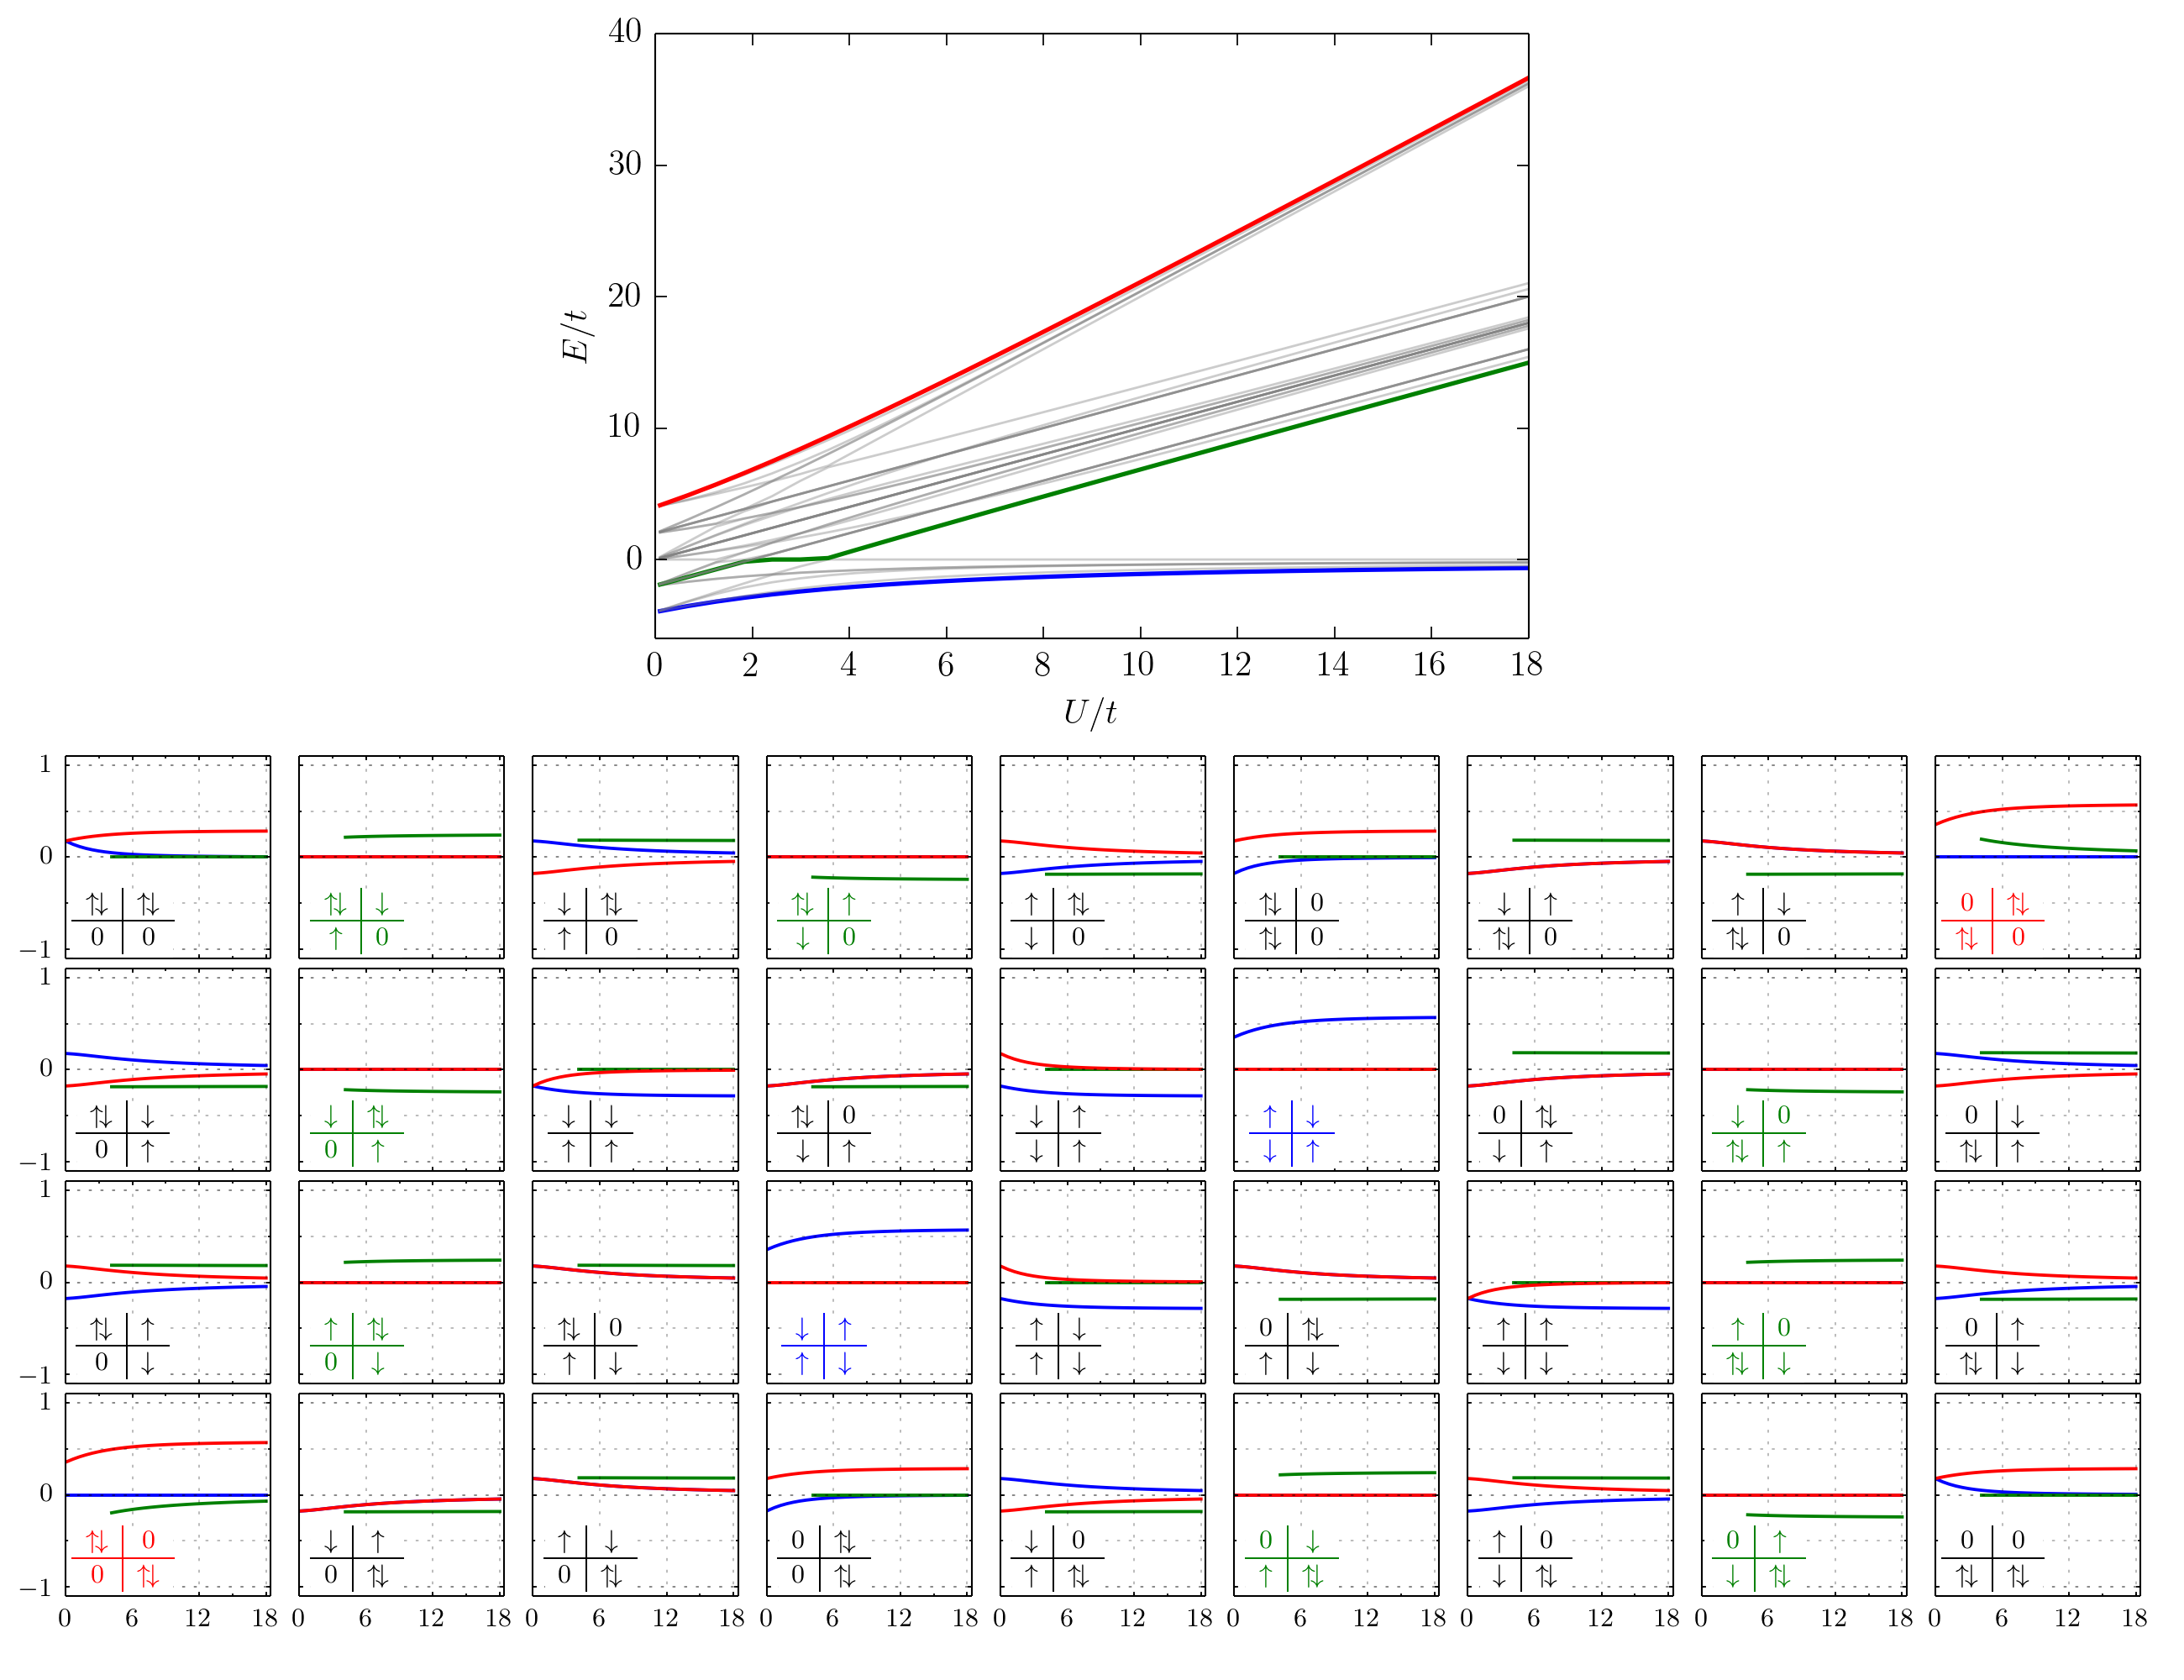
\includegraphics[width=1.0\textwidth]{../figures/hubbard/Ut_eigenvalues_4site.png}
\caption[Exact diagonalization results for a 4-site plaquette.]{\small Energy
eigenvalues and eigenstates for a 4-site plaquette.  In the top panel we show
the energy eigenvalues for all of the 36 different eigenstates.  We highlight
the ground state (blue),  the first state above the Mott-Hubbard gap (green)
and the highest energy state (red).  In the lower panels we show the
projections of each of the three highlighted states onto the basis states.
Each panel corresponds to a basis state as indicated by the diagram on the
lower left corner of the panels.  We have colored the state labels indicating
which states have the largest contribution to the eigenstates.    } 
\label{fig:exact_4site} 
\end{figure}

In the 4-site plaquette,  the largest contribution to the ground state comes
from states 
\begin{equation}
\arraycolsep=1.0pt\def\arraystretch{0.6}
  \left|
  \scalebox{0.75}{$ 
  \begin{array}{c|c}
    \nspdn & \nspup \\ \hline
    \nspup & \nspdn \\ \end{array}$ } \right\rangle =  
   a_{1\spdn}^{\dagger} a_{2\spup}^{\dagger} 
   a_{3\spup}^{\dagger} a_{4\spdn}^{\dagger} |\nvac\rangle
  ~~~~~~~~~~\text{and}~~~~~~~~~~
  \left|
  \scalebox{0.75}{$ 
  \begin{array}{c|c}
    \nspup & \nspdn \\ \hline
    \nspdn & \nspup \\ \end{array}$ } \right\rangle = 
   a_{1\spup}^{\dagger} a_{2\spdn}^{\dagger} 
   a_{3\spdn}^{\dagger} a_{4\spup}^{\dagger} |\nvac\rangle
\end{equation} 
where we have used the numbering convention
\scalebox{0.5}{\arraycolsep=1.0pt\def\arraystretch{0.7}$\begin{array}{c|c}
\makebox[1em][c]{$1$} &\makebox[1em][c]{$2$} \\ \hline \makebox[1em][c]{$3$}
&\makebox[1em][c]{$4$} \\ \end{array}$} to label the lattice sites.

There is something very important to notice in this case, though.  Going back
to the 2$\times$1 lattice we saw there was a minus sign between the two
antiferromagnetic configurations.  In this case, if we examine the panels in
Fig.~\ref{fig:exact_4site} we notice that the ground state has the largest
contributions from the antiferromagnetic configurations,  and that both
configurations show up with the same sign: 
\begin{equation} 
| \phi_{a} \rangle = 
   a_{1\spdn}^{\dagger} a_{2\spup}^{\dagger} 
   a_{3\spup}^{\dagger} a_{4\spdn}^{\dagger} |\nvac\rangle 
  ~~~~~~~~ 
|  \phi_{b} \rangle = 
   a_{1\spup}^{\dagger} a_{2\spdn}^{\dagger} 
   a_{3\spdn}^{\dagger} a_{4\spup}^{\dagger} |\nvac\rangle
\end{equation} 
As we will show, this is a consequence of the $d$-wave character of the ground
state of the 4-site plaquette at half filling.
 
The problem of a 4-site plaquette lattice should evidently be invariant to 90
degree rotations of the system about the vector normal to the lattice plane.
Four of such rotations bring the system back to the same spot, so there is an
operator $\hat{U}$, such that $\hat{U}^{4} =\mathbbm{ 1}$.  The eigenvalues of
$\hat{U}$ must therefore be $1,-1,i,-i$, each of these eigenvalues
corresponding to a different orbital symmetry.   We give an expression for
$\hat{U}$ in terms of operators that permute fermions~\cite{Gohmann1997}: 
\begin{equation} 
  \hat{U}_  = \prod_{\sigma = \spdn, \spup} 
                K_{12\sigma} K_{24\sigma} K_{43\sigma}   
\label{eq:defUrotate}
\end{equation}
The $K$ operators, which  permute fermions between two sites act as shown in
the following example: 
\begin{align} 
  K_{43\spup}  \tbtwo{\spup}{\dbl}{\spdn}{\spup}   & = 
       -\tbtwo{\spup}{\dbl}{\dbl}{0} \\
  K_{24\spup}K_{43\spup} \tbtwo{\spup}{\dbl}{\spdn}{\spup} & = 
       +\tbtwo{\spup}{\spdn}{\dbl}{\spup} \\
  K_{12\spup}K_{24\spup}K_{43\spup} \tbtwo{\spup}{\dbl}{\spdn}{\spup} & = 
       -\tbtwo{0}{\dbl}{\dbl}{\spup} \\
\end{align} 
It is seen that the combination $K_{12\spup}K_{24\spup}K_{43\spup}$ rotates all
spin ups clockwise,  which motivates the definition in Eq.~\ref{eq:defUrotate}:
first rotate the $\spdn$ spins and then rotate the $\spup$ spins to effect a
full rotation.  A formal expression for $K_{ij\sigma}$ is given by 
\begin{equation}
  K_{ij\sigma} = 1 - a_{i\sigma}^{\dagger}a_{i\sigma} 
                   - a_{j\sigma}^{\dagger}a_{j\sigma} 
                   + a_{i\sigma}^{\dagger}a_{j\sigma} 
                   + a_{j\sigma}^{\dagger}a_{i\sigma} 
\end{equation}
With the exact form for the 90 degree rotation operator in hand, we can go ahead
and apply it to the antiferromagnetic states of the 4-site plaquette to obtain
\begin{equation} 
   \hat{U} | \phi_{a} \rangle = - | \phi_{a}  \rangle
   ~~~~~~~~
   \hat{U} | \phi_{b} \rangle = - | \phi_{b}  \rangle,
\end{equation} 
thus proving the $d$-wave character of these states. The full ground state of
the 4-site plaquette also has some contributions from states with
double-occupancies and some smaller contributions from non-AFM configurations.
A complete analytical expression for the ground state, and all eigenstates in
the 4-site plaquette can be found in~\cite{Schumman2008arxiv}.  It can then be
verified that the exact ground state is an eigenstate of $\hat{U}$ with
eigenvalue -1, and thus a $d$-wave state~\cite{Schumman2008arxiv}.

\subsubsection{4-site plaquette: the connection between the Hubbard model and
$d$-wave superconductors} 

The present understanding of cuprate superconductors generally accepts a few
facts~\cite{leggett2006quantum}: 
\begin{itemize}

\item Cooper pairing is responsible for superconductivity.

\item Cooper pairs are singlet pairs with $d_{x^{2}-y^{2}}$ symmetry.  

\item Pairing occurs within the copper oxide CuO$_{2}$ planes (these planes are
a common trait of all cuprate materials).
 
\item Superconductivity occurs for a moderate amount of hole or electron doping
on a parent compound that is an antiferromagnetic Mott insulator.  
\end{itemize} 
The fact that the pairs are singlet forces their spatial wavefunction to have
even parity.  This, and the symmetry of the underlying CuO$_{2}$ square
lattice, constrains the possible orbital symmetry of the spatial part of the
wavefunction.  Experiments with Josephson junctions formed by two
superconductors have established the $d_{x^{2}-y^{2}}$ character of the spatial
part of the pair wave function~\cite{Tsuei1997,RevModPhys.72.969}.  

The simple model of a 4-site plaquette, which we saw has an antiferromagnetic
ground state with a $d$-wave orbital symmetry serves to motivate the postulate
that the Hubbard model is a very plausible model for the high-$T_{c}$ cuprates,
as we will explain below.    Considering doping on the 4-site plaquette, we can
obtain the solutions at quarter-filling, with only two electrons in the
plaquette.  Using exact diagonalization to obtain the ground state, or looking
it  up the analytical solution tables~\cite{Schumman2008arxiv},   we find that
the ground state in this case, $|\psi_{0,2}\rangle$ is an $s$-state, which
obeys 
\begin{equation}
  \hat{U} | \psi_{0,2} \rangle = + | \psi_{0,2} \rangle
\end{equation}
 
If we start out with a system of 4 particles in a plaquette, which has a
$d$-state antiferromagnetic ground state, $|\psi_{0,4}\rangle$, and want to
create a pair of holes, then the hole-pair creation operator, $\hat{\Delta}$
must satisfy
\begin{equation}
  \langle \psi_{0,2} | \hat{\Delta} | \psi_{0,4} \rangle \neq 0
\end{equation}
In other words the pairing operator must have a $d$-wave orbital symmetry, to
satisfy orbital angular momentum selection rules.  The orbital symmetry of the
pair creation operator in a 4-site plaquette is thus consistent with the
orbital symmetry of pairing observed in the high-$T_{c}$ cuprates.   This
argument, which uses the orbital symmetry of the hole-pair in a 4-site
plaquette to motivate the role of the Hubbard model in high-$T_{c}$
superconductivity, was first presented in~\cite{Scalapino1996}.
 
Another glimpse at the importance of an antiferromagnetic background for
high-$T_{c}$ superconductivity can be obtained by considering the energy of a
pair of holes in an antiferromagnetic background.   Consider the situation
shown in Fig.~\ref{fig:holepairing}, with one pair of holes.  The figure
illustrates that the energy cost of hopping, for a pair of holes, can be
limited if the hopping is correlated (the energy cost is then proportional to
the separation between holes) .  Since hopping reduces the energy by
delocalizing the holes, then it is possible for the ground state of the system
to be related to these correlated hole-pairs. 
\begin{figure} 
\centering
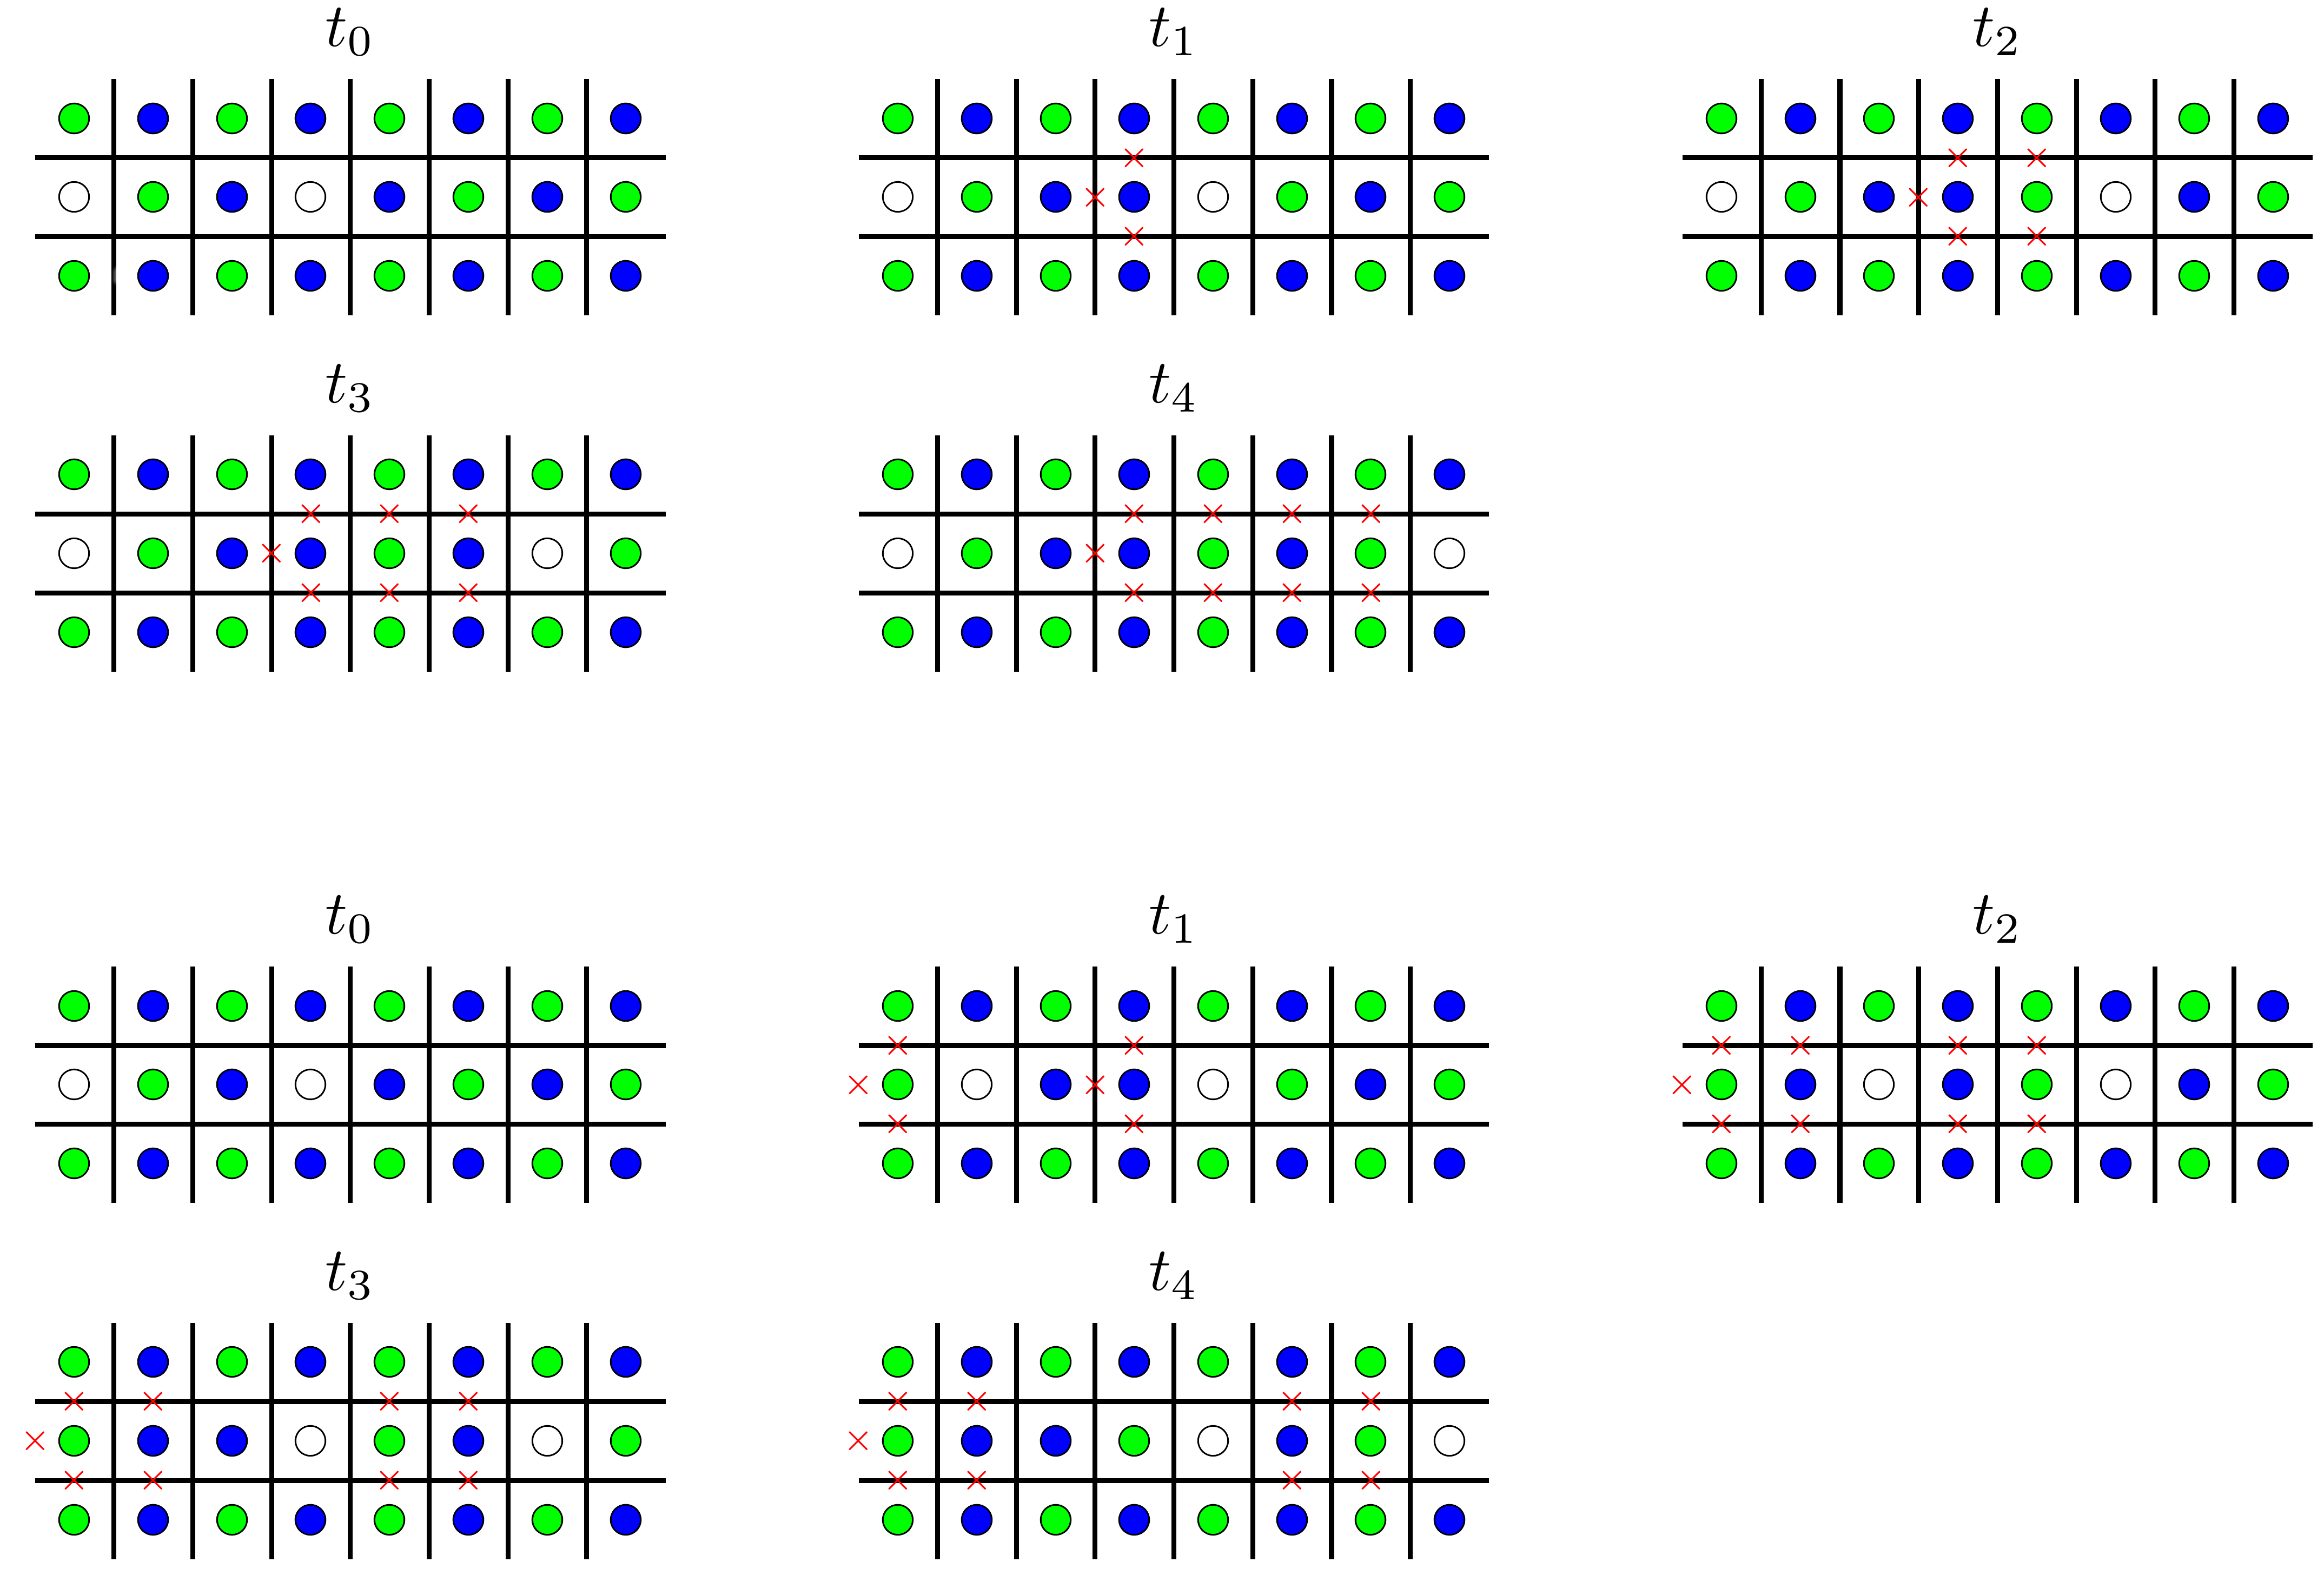
\includegraphics[width=\textwidth]{../illustrations/hole-pairing/pair_hopping.png}
\caption[Holes hopping in antiferromagnetic background.]{\small Energy
consideration for a pair of holes hopping in an antiferromagnetic background.
Spins up and down are represented as green and blue circles, holes are
represented as empty circles, and broken antiferromagnetic (AF) bonds are shown
as red crosses.  In the top series, every time the hole tunnels to an adjacent
site it breaks more AF bonds, which cost an energy $\approx -4t^{2}/{U}$ per
bond.  As the hole continues to hop, the total energy cost will be proportional
to the number of sites it has traveled.  In the bottom series, hopping is
correlated for the two holes; they hop together in the same direction.  In this
case, the energy cost of hopping will be proportional to the separation between
holes,  and it will not continue to grow as the holes move along further.   One
can see that the number of broken bonds is the same in going from $t_{3}$ to
$t_{4}$.  In the hole-doped antiferromagnet, if the kinetic energy decrease
from hole delocalization (tunneling) exceeds the cost of the broken AF bonds,
an insulating state may be able to lower its energy via the formation of
hole-pairs, } 
\label{fig:holepairing} 
\end{figure}

The arguments shown so far, regarding the symmetry of the ground states in a
4-site plaquette, and the effective attraction (or correlation) between holes
in an antiferromagnetic background, signal the close relationship between
antiferromagnetism and superconductivity.   To balance out the perspective on
this highly debated issue, we point out that in the phase diagram of
high-$T_{c}$ cuprates the  phase transition does not occur directly from an AFM
phase to a superconducting phase (the system must go through the pseudo-gap
regime as hole-doping is increased).  So if there is an AFM background in high
temperature superconductors, it may be of a different nature than the Mott
insulator type of AFM state which arises naturally in the Hubbard model. 


We hope that the simplified treatments of the Hubbard model presented so far
illustrate the richness of behaviors that emerge from it.   We have seen the
appearance of the Mott-Hubbard gap both in a single site, a double well, and a
4-site plaquette.  In the plaquette scenario we motivated the role of the
Hubbard model as one of the strongest candidates to describe the physics of
$d$-wave superconductivity in the cuprates. 
 

\section{ High-temperature series expansion } 


After exploring a few of the properties of the Hubbard model with overly
simplified approaches, we now turn to a method that will prove very useful in
comparing with experimental measurements.   The high-temperature series
expansion (HTSE) deals with tunneling as a perturbation on the on-site
interactions, and is thus the natural next step beyond the single site
treatment.  

 The partition function for the system is expanded as a series in the small
parameter $t/T$.   Clearly, this approach will work down to temperatures that
approach the tunneling rate, $T \gtrsim t$. We will see that this limits its
applicability to the calculation of thermodynamic quantities that involve the
charge degree of freedom, i.e. the density, double-occupancy, and their
derivatives.   The spin degree of freedom becomes relevant only at temperatures
below the antiferromagnetic exchange energy, which is much lower than $t$. 

We start by writing down the Hubbard Hamiltonian as  
\begin{equation}
\begin{split}
  H = &  
         \left( U\sum_{i} n_{i\spup} n_{i\spdn}  
         - \mu\sum_{i}( n_{i\spup} + n_{i\spdn} ) \right)
-t \sum_{ \langle ij \rangle, \sigma   } 
          a_{i\sigma}^{\dagger}a_{j\sigma} \\
   = &  H_{0} + H_{1} 
\end{split}
\end{equation}
We have already seen (in our treatment of the single-site model) that the
partition function for the unperturbed part, $Z_{0} = \text{Tr} e^{-\beta
H_{0}}$, factorizes as $Z_{0} = z_{0}^{k}$, for a system with $k$ sites.  The
single site partition function  is easy to calculate because the trace runs
over the only four possible states in a single site $\lbrace |0\rangle,
|\spup\rangle, |\spdn\rangle, |\dbl\rangle\rbrace$.
\begin{equation}
 z_{0} = 1 + 2 e^{\beta\mu} + e^{\beta (2\mu-U)} = 1 + 2z + z^{2}u 
\end{equation}
where we have defined $z=e^{\beta\mu}$ and $u=e^{-\beta U }$ 



For the full Hamiltonian, the grand canonical partition function $Z$ can be
expanded in a perturbation series~\cite{mahan2000many,Henderson1992} 
\begin{equation}
\begin{split}
  Z = & \text{Tr} e^{-\beta H}  \\
    = & Z_{0} \left[ 1 + 
        \sum_{n=1}^{\infty} (-1)^{n} 
        \int_{0}^{\beta} d\tau_{1} \int_{0}^{\tau_{1}} d\tau_{2} 
        \dotsm \int_{0}^{\tau_{n-1}} d\tau_{n} 
        \langle
              \tilde{H}_{1}(\tau_{1}) 
              \tilde{H}_{1}(\tau_{2})  \dotsm
              \tilde{H}_{1}(\tau_{n})  \rangle 
              \right] 
\end{split}
\end{equation} 
where the thermal expectation value inside the integrals is taken with the
unperturbed part of the Hamiltonian
\begin{equation}
\langle A \rangle = \text{Tr} ( e^{\beta H_{0} } A ) / Z_{0} , 
\end{equation}
and the tilde means that the operator is evaluated in the interaction picture
for the imaginary time in parenthesis: 
\begin{equation}
 \tilde{H}_{1}(\tau) = e^{\tau H_{0}} H_{1} e^{-\tau H_{0}} 
\end{equation}
Given the series expansion for $Z$, the grand potential is 
\begin{equation}
 -\beta \Omega = Z_{0} + 
        \sum_{n=1}^{\infty} (-1)^{n} 
        \int_{0}^{\beta} d\tau_{1} \int_{0}^{\tau_{1}} d\tau_{2} 
        \dotsm \int_{0}^{\tau_{n-1}} d\tau_{n} 
        \langle
              \tilde{H}_{1}(\tau_{1}) 
              \tilde{H}_{1}(\tau_{2})  \dotsm
              \tilde{H}_{1}(\tau_{n})  \rangle 
\end{equation}

One can see that the $n^{th}$ term in the expansion has $n$ copies of the
tunneling part of the Hamiltonian.  In the thermal average, each  application
of $H_{1}$ results in a particle tunneling to a neighboring site. We see that
there will be a contribution to the expansion only if after $n$ tunneling
events all the particles come back to their original sites.  A direct
consequence of this is that the first order term in the expansion vanishes (you
cannot recover the same lattice configuration after a single tunneling event).
The second order in the expansion corresponds to particles tunneling one site
over and then coming back.  Higher order terms can be represented by diagrams,
to make them easier to keep track off.  The contribution from orders up to
$n=9$ is shown in~\cite{Henderson1992}.  Here we will use up to the second
order term to illustrate the phases that appear in the system.  

The grand potential to second order is~\cite{Henderson1992,Jordens2010} 
\begin{equation}
-\beta \Omega_{2} = k \ln z_{0} + k \left( \frac{\beta t }{z_{0}} \right)^{2} m 
        \left( z + z^{3} u + 2z^{2} \frac{1-u}{\beta U} \right) 
\end{equation} 
where $m$ is the number of nearest neighbors for each lattice site, which in
the simple cubic case is $m=6$.  We see that the grand potential is
proportional to the number of lattice sites, so we will obtain all the
thermodynamic quantities per lattice site. 

\begin{figure}
\centering
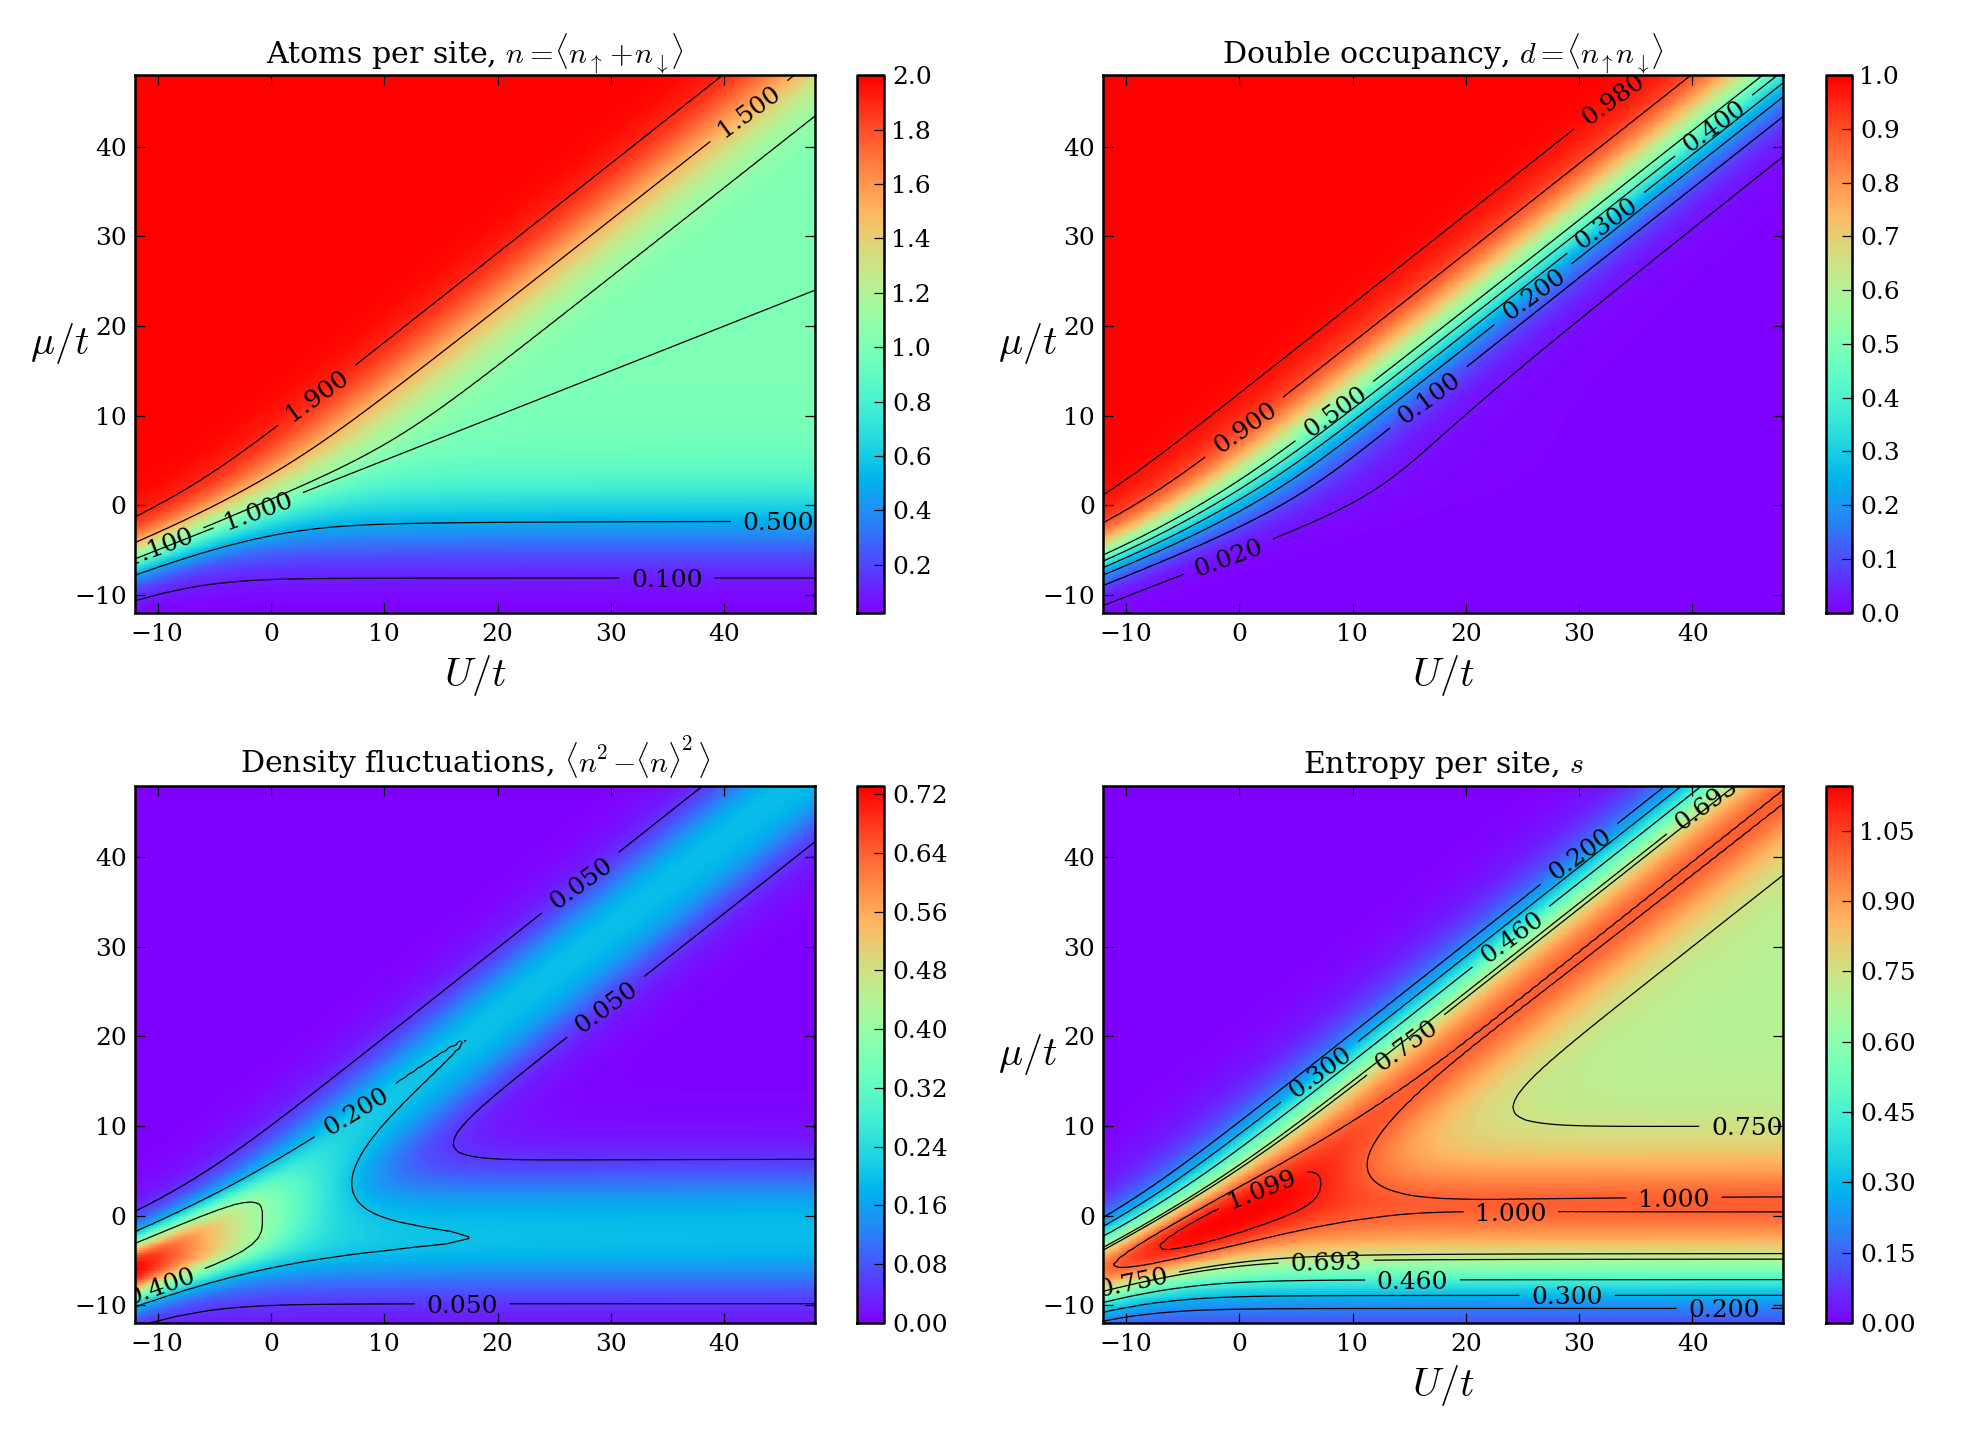
\includegraphics[width=\textwidth]{../figures/HubbardPhaseDiagram_figures/HTSE_phasesT025.png}
\caption[HTSE state diagram of the Fermi-Hubbard model]{\small HTSE state
diagram of the Fermi-Hubbard model calculated up to second order in the
perturbation series.  } \label{fig:highTphases}
\end{figure}
From the grand potential to second order we can calculate a state diagram for
the Hubbard model.  In Fig.~\ref{fig:highTphases}, the results are shown at a
temperature $T=2.5t$. Constant $T/t$ cuts are shown for different temperatures
in Fig.~\ref{fig:HTSEhomogeneous}.  

From the figures, we see that the HTSE up to second order exhibit the main
features of the Mott insulating regime: 
\begin{itemize}
\item The density as function of chemical potential has a
plateau at $n=1$ centered around $\mu=U/2$, Fig.\ref{fig:HTSEhomogeneousA}.
\item At $n=1$ the double occupancy
is suppressed for lower temperatures, Fig.~\ref{fig:HTSEhomogeneousB}.
\item
At $n=1$ the density fluctuations are suppressed, Fig.~\ref{fig:HTSEhomogeneousC}.
\item At $n=1$ the entropy per site is lowered,
Fig.~\ref{fig:HTSEhomogeneousD}.
\end{itemize}
For very large values of $U/t$, where at $T=2.5t$ we have $T \ll U$, the system
is deep in the Mott insulator regime.  The system has exactly one atom per
site, and the only remaining entropy is the spin entropy.  With two spin states
available per lattice site, the entropy per lattice site is $s = \ln 2 \approx
0.7 $, as can be seen in the third panel of Fig.~\ref{fig:HTSEhomogeneousD}.  

\begin{figure}
        \centering
        \begin{subfigure}[b]{0.48\textwidth}
                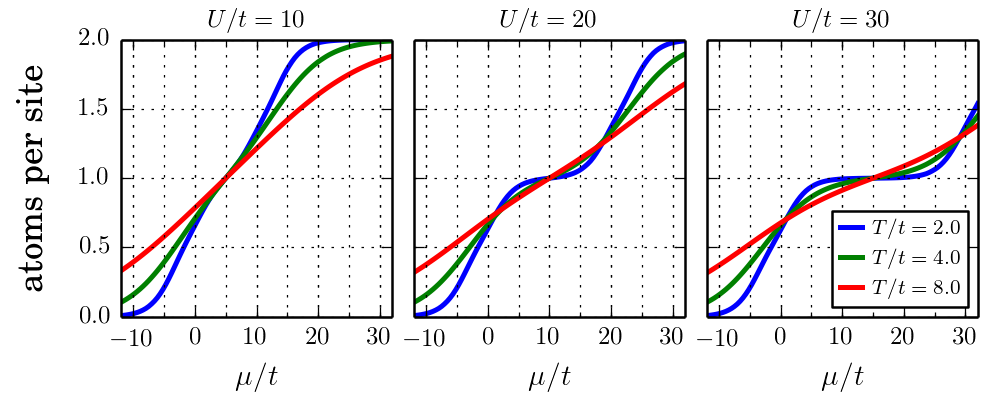
\includegraphics[width=\textwidth]{../figures/lda_evap/HTSE_density_U.png}
                \caption{Density}
\label{fig:HTSEhomogeneousA}
        \end{subfigure}%
          %add desired spacing between images, e. g. ~, \quad, \qquad etc.
          %(or a blank line to force the subfigure onto a new line)
        ~
        \begin{subfigure}[b]{0.48\textwidth}
                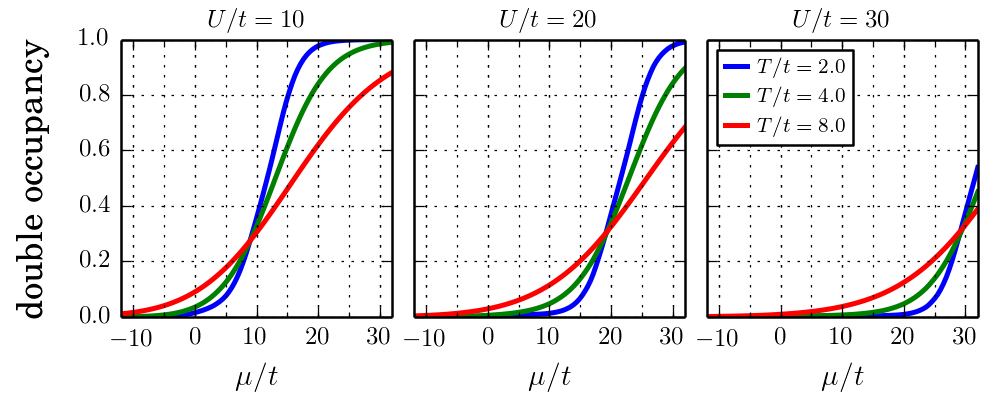
\includegraphics[width=\textwidth]{../figures/lda_evap/HTSE_doublons_U.png}
                \caption{Double occupancy}
\label{fig:HTSEhomogeneousB}
        \end{subfigure}

        \begin{subfigure}[b]{0.48\textwidth}
                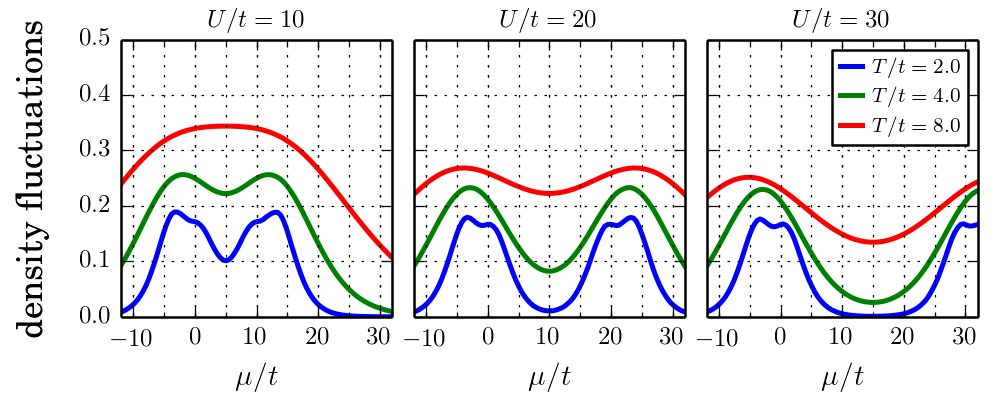
\includegraphics[width=\textwidth]{../figures/lda_evap/HTSE_densfluc_U.png}
                \caption{Density fluctuations}
\label{fig:HTSEhomogeneousC}
        \end{subfigure}
        ~
        \begin{subfigure}[b]{0.48\textwidth}
                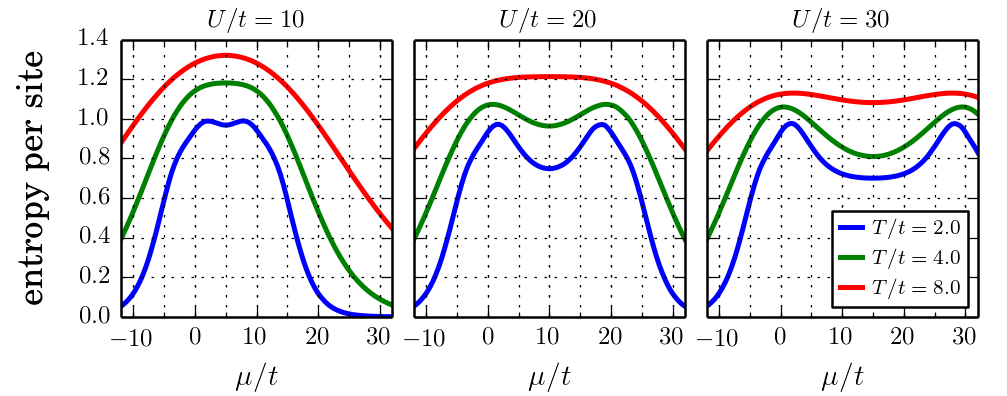
\includegraphics[width=\textwidth]{../figures/lda_evap/HTSE_entropy_U.png}
                \caption{Entropy per lattice site}
\label{fig:HTSEhomogeneousD}
        \end{subfigure}
        \caption{\small Thermodynamic quantities as a function of chemical potential calculated using the HTSE.}
\label{fig:HTSEhomogeneous}
\end{figure}


We can also plot the HTSE result for the entropy as a function of density, as
shown in Fig.~\ref{fig:HTSE_spersite}.  Dividing the entropy per lattice site
by the density, we obtain the entropy per particle, shown in
Fig.~\ref{fig:HTSE_sperparticle}.  The entropy per particle rises significantly
at lower densities, which indicates the large entropy capacity of the metallic
phase. 

\begin{figure}
        \centering
        \begin{subfigure}[b]{0.65\textwidth}
    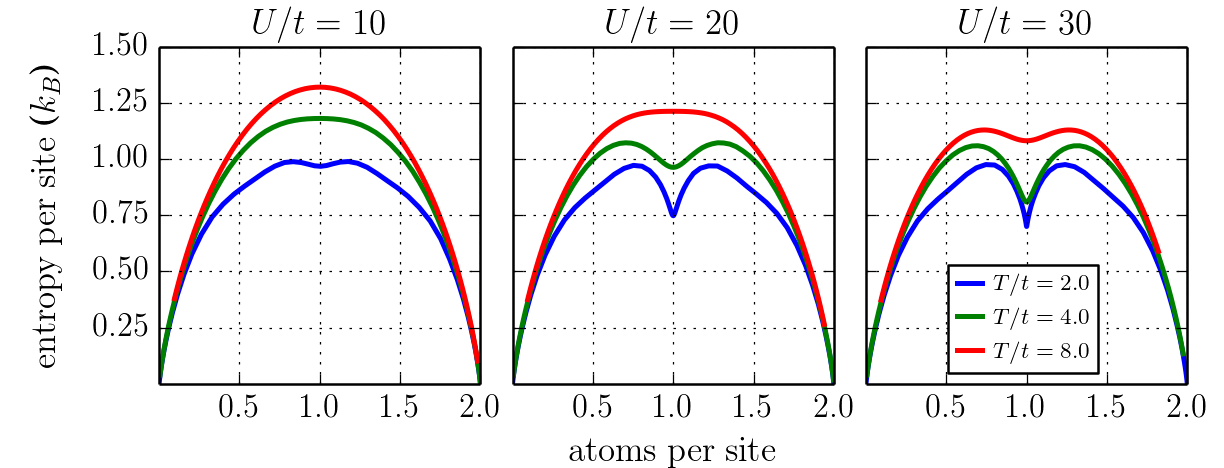
\includegraphics[width=\textwidth]{../figures/lda_evap/HTSE_EntropyPerSite_U.png}
    \caption{Entropy per lattice site versus density.}\label{fig:HTSE_spersite}
     \end{subfigure}

\begin{subfigure}[b]{0.65\textwidth}
    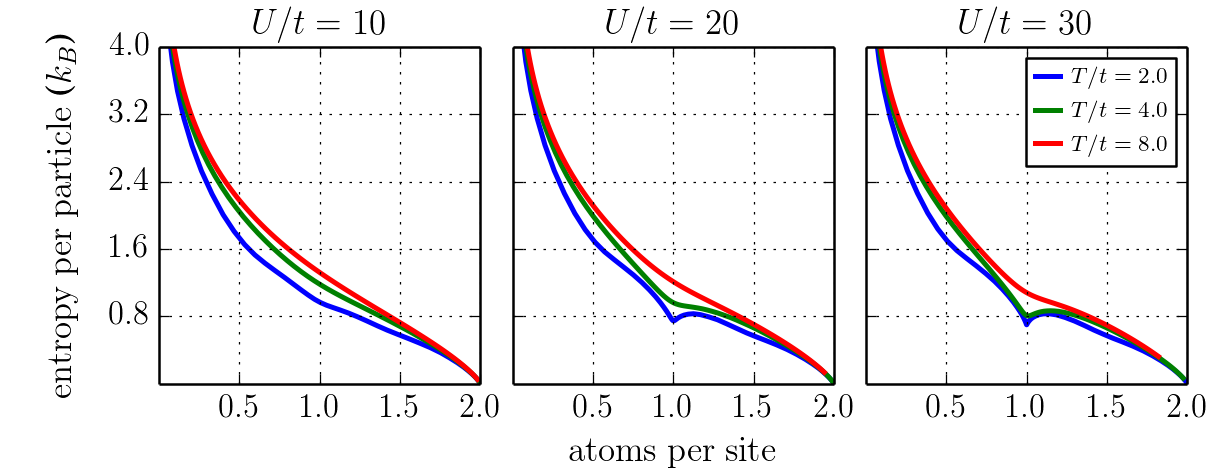
\includegraphics[width=\textwidth]{../figures/lda_evap/HTSE_EntropyPerParticle_U.png}
    \caption{Entropy per particle versus density.}\label{fig:HTSE_sperparticle}
   \end{subfigure}
\end{figure}

In a finite trapped system which inevitably has a shell with density $n<1$ , a
large part of the total entropy of the system is carried by particles in the
low density shell.  This \textbf{entropy redistribution} allows the core to be
at an effectively lower entropy per particle.  The core can then locally access
lower entropy phases, such as the AFM state,  even if the overall value of the
entropy per particle is larger than the N\'{e}el entropy for a homogeneous
system\footnote{ For the homogeneous system the N\'{e}el entropy per particle
(at which the Mott insulator becomes AFM ordered) is $s_{\text{N\'{e}el}} = 0.4
k_{\text{B}}$}.  We will elaborate more on this later on when we describe our
trapping potential. 


\section{ Local density approximation }

The results presented above consider a homogeneous lattice potential.  In
experiments with ultracold atoms,  a confining potential is a necessity since
the samples created have a finite number of atoms.  The presence of an
inhomogeneous overall trapping potential presents a major challenge when
comparing the results of experiment to theory.  A useful technique, which works
for systems without long range correlations, is the local density approximation
(LDA) .  In the LDA, we consider each point in the potential as an homogeneous
system and we set the condition that all of these local homogeneous systems are
in thermal equilibrium with each other  at some temperature $T$.  If the
trapping potential is properly characterized,  at each point we can obtain a
local value of the lattice depth, which along with the scattering length (set
for the whole system via a Feshbach resonance), determines the local values of
the Hubbard parameters $t$ and $U$.  With the Hubbard parameters in hand, we
can use a known solution to the homogeneous Hubbard model and obtain local
values for the thermodynamic quantities, such as density, double occupancy,
entropy, etc.   We can then plot the local thermodynamic quantities as a
function of trap position to obtain trap profiles.  Alternatively, one can also
integrate the results of the LDA over the trap and compare them to bulk
measurements. 


The validity of the LDA in lattice systems has been addressed
before~\cite{Rigol2003,Helmes2008,Chiesa2011},  proving that it yields very
good agreement with exact calculations of the trap for quantities such as
density profiles and momentum distributions and only slight discrepancies with
quantities like the spectral function of the many-body excitations.  In the
work carried out for this thesis, all the comparisons with theory were done
within the framework of the LDA. 


\section{Latest developments in numerical techniques}

When performing the LDA one needs to have available a set of results for a
homogeneous model with data available at low enough temperatures to match those
of the experiment.   In our experiment the temperature can be as low as
$T/t\approx0.4$ locally, just above $T_{N}$ and so we need to make use of the
latest developments in numerical techniques to access this regime.   The hope
is that one day ultracold atoms will greatly exceed the capabilities of
numerical calculations, such that open questions like that of $d$-wave
superconductivity in the Hubbard model can be put to rest. 

Going down to temperatures comparable to the tunneling rate ($T<t$), analytical
methods such as the HTSE up to second order fall short in their ability to
describe the thermodynamics of the Hubbard model.  Below these temperatures a
variety of more sophisticated approaches has been used in the literature.
Below we provide a non-exhaustive list of the main methods that have been
applied to ultracold atoms in optical lattices:  

\begin{itemize} 

\item \textbf{DMFT}.  Dynamical mean field theory. It considers a single site
of the lattice, $H_{1}= Un_{\spup}n_{\spdn} - \mu (n_{\spup} + n_{\spdn})$,
immersed in a bath of non-interacting electrons which represents the rest of
the system.   The interaction between the bath and the impurity is mapped onto
what is referred to as a single-impurity Anderson model.    The resulting
impurity model is solved with a self-consistency condition, i.e.  the resulting
dynamics of the bath must be consistent with the dynamics of the impurity
since, after all, the bath is made of a bunch of other sites, just like the one
under consideration.  Of course, this is easier said than done; nevertheless,
the problem reduces to solving the problem for a single-impurity.  There are
several techniques available for that task.  Ref.~\cite{Helmes2008} uses the
numerical renormalization group (NRG), for example. 


\item \textbf{DCA}.  Dynamical cluster approximation.  This is an extension of
DMFT, where the impurity is not a single site but a cluster of sites.  As the
number of sites in the cluster, $N_{c}$ goes to infinity one should recover the
exact solution, and for $N_{c}=1$ the method reduces to DMFT.   The DCA was used
to calculate the thermodynamics of the Fermi-Hubbard in a 3D lattice in
Ref.~\cite{Fuchs2011}.

\item \textbf{DQMC}.  Determinantal quantum Monte Carlo.  In general, the Monte
Carlo  method reduces the calculation of the full quantum partition function as
a sum over all possible configurations in some product space basis set (where
the basis states are products of single particle states).  In
DQMC~\cite{Scalettar:hubbardIII,PhysRevD.24.2278}, an exact simplification is
used where the partition function is reduced to a sum over the determinant of
the Hamiltonian matrix (in the chosen basis).  So the name ``determinantal''
QMC.  This simplification holds if the Hamiltonian is quadratic.  The on-site
interaction term in the Hubbard model is quartic instead of quadratic, but
there is a way to handle this using what is called a Hubbard-Stratonovich
transformation.  A problem with applying this method to fermions is that the
determinant of the resulting matrices can be negative sometimes, which affects
the convergence of the Monte Carlo evaluation of the sum.   This is known as
the sign problem,  it can be avoided completely for calculations at
half-filling ($\mu=U/2$) and it is not so significant for small values of $U$ at
arbitrary filling.  However, for large values of $U \gtrsim 12$ it prevents
calculations for values of $T/t \lesssim 1$. 

\item \textbf{NLCE}. Numerical linked-cluster expansion.   The NLCE is a series
expansion in powers of $t/T$, which reminds one of the HTSE.  In the HTSE,
different contributions are grouped solely by the power of $t/T$, whereas in
the NLCE clusters of sites are exactly diagonalized (numerically) and added to
the series according to a weight that can be obtained by a considering all
possible subclusters in the cluster~\cite{PhysRevLett.97.187202}.   The region
of convergence of the NLCE can be extended for  $T/t<1$ via numerical
resummations~\cite{Tang2013}, although results for $T/t<0.8$ in a 3D lattice
can get rather noisy, as we will see. 

\end{itemize}

As part of this thesis we have closely collaborated with the following condensed matter theorists:
\begin{itemize}
\item Thereza Paiva at Universidade Federale de Rio de Janeiro  
\item Ehsan Khatami at San Jose State University
\item Richard Scalettar at UC Davis
\item David Huse at Princeton University
\item Nandini Trivedi at Ohio State University
\end{itemize}  

Our collaborators are experts in the use of DQMC and NLCE and so all of the
modeling of our experimental results is restricted to these two techniques.
